%%%%%%%%%%%%%%%%%%%%%%%%%%%%%%%%%%%%%%%%%%%%%%%%%%%%%%%%%%%%%%%%%%%%%%%%%%%%%%%%
%%%%%%%%%%%%%%%%%%%%%%%%%%%%%%%%%%%%%%%%%%%%%%%%%%%%%%%%%%%%%%%%%%%%%%%%%%%%%%%%
%%                           AUTHOR: BIBEKANANDA DATTA                        %%
%%                               (C) MARCH 2024                               %%
%%                      PhD STUDENT, MECHANICAL ENGINEERING                   %%
%%                           JOHNS HOPKINS UNIVERSITY                         %%
%%%%%%%%%%%%%%%%%%%%%%%%%%%%%%%%%%%%%%%%%%%%%%%%%%%%%%%%%%%%%%%%%%%%%%%%%%%%%%%%
%%%%%%%%%%%%%%%%%%%%%%%%%%%%%%%%%%%%%%%%%%%%%%%%%%%%%%%%%%%%%%%%%%%%%%%%%%%%%%%%
%%             PLEASE CHECK THE README.md FILE BEFORE YOU PROCEED             %%
%%              it may be convenient to read this file on GitHub              %%
%%   GitHub: https://github.com/bibekananda-datta/JHU-Dissertation-Template   %%
%% template hosted on this GitHub repository is likely to be the most updated %%
%%%%%%%%%%%%%%%%%%%%%%%%%%%%%%%%%%%%%%%%%%%%%%%%%%%%%%%%%%%%%%%%%%%%%%%%%%%%%%%%

%%%%%%%%%%%%%%%%%%%%%%%%%%%%%%%%%%%%%%%%%%%%%%%%%%%%%%%%%%%%%%%%%%%%%%%%%%%%%%%%
% This is an unofficial dissertation template for Johns Hopkins University.
% As of March 31, 2024, the template follows the dissertation formatting 
% requirements provided by the  Johns Hopkins University Sheridan Library.
% It is the user's responsibility to ensure that the current requirements are 
% followed: https://www.library.jhu.edu/library-services/electronic-theses-dissertations/formatting-requirements/
%%%%%%%%%%%%%%%%%%%%%%%%%%%%%%%%%%%%%%%%%%%%%%%%%%%%%%%%%%%%%%%%%%%%%%%%%%%%%%%%
%%%%%%%%%%%%%%%%%%%%%%%%%%%%%% VERSION HISTORY %%%%%%%%%%%%%%%%%%%%%%%%%%%%%%%%%
% The report class-based template was created by R. Jacob Vogelstein in May 2007
% Updated by Noah J. Cowan on March 01, 2010
% Updated by Brian D. Weitzner on April 29, 2014 
% Updated by John Muschelli on January 29, 2016 
% Updated by Leonardo Collado Torres on April 13, 2016 
% Updated by John Clayton in December 2019
% Last Updated by Bibekananda Datta on March 31, 2024
%%%%%%%%%%%%%%%%%%%%%%%%%%%%%% VERSION HISTORY %%%%%%%%%%%%%%%%%%%%%%%%%%%%%%%%%


%%%% REPORT CLASS with 12 pt font and onesided printing (book class also works)
\documentclass[12pt,letterpaper]{report} 

%%%%%%%%%%%%%%%%%%%%%%%%%%%%%%%%%%%%%%%%%%%%%%%%%%%%%%%%%%%%%%%%%%%%%%%%%%%%%%%%
%% if possible, make your formatting changes here through the variables 
%%%%%%%%%%%%%%%%%%%%%% LIST OF VARIABLES FOR FORMATTING %%%%%%%%%%%%%%%%%%%%%%%%

%%%% JH Library requirement (DO NOT CHANGE)
\def\GlobalMargin{1.0in}                    % margin on all sides
\def\PrintingOffset{0in}                  % additional left margin for the printed copy
\def\MainTextSpacing{\doublespacing}        % double-spaced main text


%%%% ADDITIONAL PATHS and FILES
\def\FigurePath{figures}                    % subdirectory for the figure files
\def\BibFileName{thesis.bib}                % name of BibLaTeX-compatible bib file 


\def\FontPackage{lmodern}                   % default font package

\def\HyperlinkColor{blue}                   % color for hyperlinks


%%%% FONT SIZE and TYPESET for DIFFERENT HEADINGS
%% check here for details: https://en.wikibooks.org/wiki/LaTeX/Fonts
%% font format for thesis title
\def\TitleFont{\Large\bfseries\singlespacing\MakeUppercase}  

%% font for chapter, section, subsection, and subsubsection heading
\def\NoSectionLevel{3}                      % 3 levels => section to subsubsection
\def\ChapterFont{\Large\bfseries\singlespacing} 
\def\SectionFont{\large\bfseries\singlespacing} 
\def\SubsectionFont{\normalsize\bfseries\singlespacing}  
\def\SubsubsectionFont{\normalsize\itshape\singlespacing} 


%%%% PARAGRAPH
\def\ParagraphSpacing{\baselineskip}        % spacing between paragraph
\def\ParagraphIndent{0 pt}                  % indentation at the beginning of the paragraph


%% CAPTION
\def\CaptionFontSize{small}                 % caption font size
\def\CaptionLabelFontType{bf}               % boldface label for captions
\def\CaptionSeparator{colon}                % separates caption label from caption text
\def\CaptionSpacing{1.0}                    % single-spaced captions
\def\FigureToCaption{0 pt}                  % spacing between the figure and the caption


%%%% GLOBAL SPACING for TABLES
\def\GlobalTableSpacing{1.5}                % global spacing parameter for table


%%%% HEADER AND FOOTER SETTING
\def\HeaderHeight{30 pt}                    % height of the chapter header
\def\HeaderSpace{12 pt}                     % space between header and the following text

\def\FootnoteSpacing{\baselineskip}         % spacing between footnotes


%%%% BIBLIOGRAPHY ITEMS
\def\BibTextSpacing{\singlespacing}         % single-spaced bibliography
\def\BibItemSpacing{\baselineskip}          % spacing between bibliographic items in reference


%%%% CHAPTER QUOTE (EPIGRAPH PACKAGE)
\def\ChapQuoteFontSize{\small}              % font size of chapter quotes
\def\ChapQuoteLocation{flushright}          % location of chapter quote
\def\ChapQuoteTextShape{\itshape}           % font shape for quotes
\def\ChapQuoteAuthorTextShape{\scshape}     % font shape for quote author
\def\MaxQuoteWidth{0.65\textwidth}          % width epigraph-based quotes in chapter



%%%% SECTION LEVELS and TOC APPEARANCE
\def\NoTOCLevel{2}                          % no of levels showed in the table of contents
\def\TOCIndent{0 pt}                        % indentation in the list of figs and tables
%% 3 levels mean: section to subsubsection.. decrease if you want to show less in TOC


%%%% TOC SPACING of different section levels (chapter to subsubsection)
\def\TOCTextSpacing{\singlespacing}         % single spacing for TOC texts
\def\ChapTOCSpacing{\baselineskip}          % spacing between chapters
\def\SecTOCSpacing{0.5\baselineskip}        % spacing between sections
\def\SubsecTOCSpacing{0.3\baselineskip}     % ... between subsections
\def\SubsubsecTOCSpacing{0.3\baselineskip}  % ... between subsubsections
\def\LOTItemSpacing{\baselineskip}          % spacing between LOT/LOF items



%%%% ADHOC HEIGHT ADJUSTMENT VARIABLES for consistent typesettings
%% following numbers are found by trial and error to compensate 
%% for the default spacing around different LaTeX environments.
%% unless you find inconsistent formatting, you may not need to change these
\def\TitleTopSpacing{-\HeaderHeight-\HeaderSpace}   % top height adjustment for thesis title
\def\BeforeTOCTitleSpacing{-42 pt}          % space before TOC title
\def\AfterTOCTitleSpacing{34 pt}            % space after TOC title
\def\AfterLOTTitleSpacing{34 pt}            % space after LOT/ LOF title

\def\NumChapterTopMargin{-64 pt}            % space before numbered chapter label
\def\UnNumChapterTopMargin{-85 pt}          % space before unnumbered chapter label
\def\ChapLabelToTitle{-27 pt}               % space between chapter label to title 
\def\ChapTitleToText{24 pt}                 % space between the chapter title and the following text
\def\SpaceBeforeQuote{-20 pt}               % white space before quote

%%%% if you want to change any of the heights, adjust using a ruler:
% \usepackage[unit=in,type=upperleftT,color=red,showframe]{fgruler}

%%%%%%%%%%%%%%%%%%%% END LIST OF VARIABLES FOR FORMATTING %%%%%%%%%%%%%%%%%%%%%%


%%%%%%%%%%%%%%%%%%%%%%%%%%%%%%%%%%%%%%%%%%%%%%%%%%%%%%%%%%%%%%%%%%%%%%%%%%%%%%%%
%% add packages as needed but sometimes the order of the packages matters.
%% you may have to change the options of the biblatex package for the bibliography.
%%%%%%%%%%%%%%%%%%%%%%%%%%%%%%% LaTeX PACKAGES %%%%%%%%%%%%%%%%%%%%%%%%%%%%%%%%%

%%%% SOME PRE-REQUISITE PACKAGES
\usepackage[utf8]{inputenc}                 % for encoding input character (required)
% Declare the stray combining acute accent so LaTeX maps it to \'{}
\DeclareUnicodeCharacter{0301}{\'{}}
\DeclareUnicodeCharacter{0302}{\'{}}
% Declare the stray combining acute accent so LaTeX maps it to \'{}
\DeclareUnicodeCharacter{0308}{\'{}}
\usepackage[american]{babel}                % for different language typography
\usepackage[T1]{fontenc}                    % for font encoding


%%%% DEFAULT FONT (you can specify other fonts - compatibility could be an issue)
\usepackage{\FontPackage}


%%%% COMMON MATH PACKAGES
\usepackage{amsfonts,amssymb,amsmath,amsthm,autobreak,
    cancel,dsfont,mathtools,mathbbol,mathrsfs,siunitx,upgreek}


%%%% TABLE-RELATED PACKAGES
\usepackage{booktabs,longtable,dcolumn,makecell,
    multicol,multirow,tabularx,xltabular,rotating}


%%%% package for micro-typography (you can define more settings)
%% see details here: https://www.khirevich.com/latex/microtype/
\usepackage[activate={true,nocompatibility}]{microtype}



%%%% BIBLIOGRAPHIC PACKAGE (change the style or other options if you need to)
%% Nature style bibliography
%\usepackage[backend=biber, defernumbers=true, style=nature, maxnames=99, natbib=true,
%     date=year, isbn=false, url=false, doi=true]{biblatex}

%% APA style
%\usepackage[backend=biber, defernumbers=true, style=apa, maxnames=99, natbib=true,
%     isbn=false, url=false, doi=true]{biblatex}

%% IEEE style
%\usepackage[backend=biber,style=ieee,defernumbers=true,maxnames=99, natbib=true,
%     date=year, isbn=false, url=false, doi=true]{biblatex}

\usepackage[backend=biber,
            style=authoryear,  % ← author–year
            natbib=true,       % still allows \citet/\citep
            maxcitenames=2,    % “Einstein et al.”
            maxbibnames=99,
            date=year,
            isbn=false,
            url=false,
            doi=true
           ]{biblatex}



%%%% OTHER PACKAGES AND OPTIONS
\usepackage[pagewise,mathlines]{lineno}     % line numbers for drafting
\usepackage[ruled]{algorithm2e}             % to manage algorithm environment
\usepackage[titletoc]{appendix}             % to manage appendix chapters
\usepackage{blindtext}                      % to generate random filler texts
\usepackage{calc}                           % to set arithmetic arguments for spacing
\usepackage{caption}                        % to manage captions
\usepackage{comment}                        % to comment a large amount of text as env
\usepackage{epigraph,varwidth}              % for managing quotes
\usepackage{enumitem}                       % to manage list environment
\usepackage{float}                          % to manage floating environment
% footnote environment management
\usepackage[bottom,multiple,hang,flushmargin]{footmisc}      
\usepackage{graphicx,wrapfig}               % to manage images
\usepackage{geometry}                       % to manage margins and page format
\usepackage{glossaries}                     % to add glossaries
\usepackage{fancyhdr}                       % for header/ footer settings
\usepackage[dvipsnames]{xcolor}             % color-related package
\usepackage[a-1b]{pdfx}                     % to generate PDF/A file (add before hyperref)
\usepackage[pdfa]{hyperref}                 % for hyperlink management 
\usepackage[all]{hypcap}                    % for captions on the side of figures
\usepackage{ifthen}                         % if-then statement in LaTeX code
\usepackage{lscape}                         % landscape mode
\usepackage{listings,minted}                % to include codes 
\usepackage{csquotes}                       % yet another package to manage quote
\usepackage{setspace}                       % sets space between lines
\usepackage{seqsplit}                       % splits long character sequence
\usepackage[rightcaption]{sidecap}          % for sideway captions
\usepackage{tocloft}                        % to manage table of contents, etc.
\usepackage{textcomp}                       % text companion fonts in TS1
\usepackage[absolute]{textpos}              % position text at certain location
\usepackage{titlesec}                       % managing different title environments
\usepackage[final]{pdfpages}                % to insert pdf pages
\usepackage{parskip}                        % default spacing around environments
\usepackage{tikz}                           % drawing related package
\usepackage{subcaption}                     % individual panel and caption

\usepackage[most]{tcolorbox}
\usepackage{soul}
%%%%% NEW MATH DEFINITIONS %%%%%

\usepackage{amsmath,amsfonts,bm}

% Mark sections of captions for referring to divisions of figures
\newcommand{\figleft}{{\em (Left)}}
\newcommand{\figcenter}{{\em (Center)}}
\newcommand{\figright}{{\em (Right)}}
\newcommand{\figtop}{{\em (Top)}}
\newcommand{\figbottom}{{\em (Bottom)}}
\newcommand{\captiona}{{\em (a)}}
\newcommand{\captionb}{{\em (b)}}
\newcommand{\captionc}{{\em (c)}}
\newcommand{\captiond}{{\em (d)}}

% Highlight a newly defined term
\newcommand{\newterm}[1]{{\bf #1}}


% Figure reference, lower-case.
\def\figref#1{figure~\ref{#1}}
% Figure reference, capital. For start of sentence
\def\Figref#1{Figure~\ref{#1}}
\def\twofigref#1#2{figures \ref{#1} and \ref{#2}}
\def\quadfigref#1#2#3#4{figures \ref{#1}, \ref{#2}, \ref{#3} and \ref{#4}}
% Section reference, lower-case.
\def\secref#1{section~\ref{#1}}
% Section reference, capital.
\def\Secref#1{Section~\ref{#1}}
% Reference to two sections.
\def\twosecrefs#1#2{sections \ref{#1} and \ref{#2}}
% Reference to three sections.
\def\secrefs#1#2#3{sections \ref{#1}, \ref{#2} and \ref{#3}}
% Reference to an equation, lower-case.
\def\eqref#1{equation~\ref{#1}}
% Reference to an equation, upper case
\def\Eqref#1{Equation~\ref{#1}}
% A raw reference to an equation---avoid using if possible
\def\plaineqref#1{\ref{#1}}
% Reference to a chapter, lower-case.
\def\chapref#1{chapter~\ref{#1}}
% Reference to an equation, upper case.
\def\Chapref#1{Chapter~\ref{#1}}
% Reference to a range of chapters
\def\rangechapref#1#2{chapters\ref{#1}--\ref{#2}}
% Reference to an algorithm, lower-case.
\def\algref#1{algorithm~\ref{#1}}
% Reference to an algorithm, upper case.
\def\Algref#1{Algorithm~\ref{#1}}
\def\twoalgref#1#2{algorithms \ref{#1} and \ref{#2}}
\def\Twoalgref#1#2{Algorithms \ref{#1} and \ref{#2}}
% Reference to a part, lower case
\def\partref#1{part~\ref{#1}}
% Reference to a part, upper case
\def\Partref#1{Part~\ref{#1}}
\def\twopartref#1#2{parts \ref{#1} and \ref{#2}}

\def\ceil#1{\lceil #1 \rceil}
\def\floor#1{\lfloor #1 \rfloor}
\def\1{\bm{1}}
\newcommand{\train}{\mathcal{D}}
\newcommand{\valid}{\mathcal{D_{\mathrm{valid}}}}
\newcommand{\test}{\mathcal{D_{\mathrm{test}}}}

\def\eps{{\epsilon}}


% Random variables
\def\reta{{\textnormal{$\eta$}}}
\def\ra{{\textnormal{a}}}
\def\rb{{\textnormal{b}}}
\def\rc{{\textnormal{c}}}
\def\rd{{\textnormal{d}}}
\def\re{{\textnormal{e}}}
\def\rf{{\textnormal{f}}}
\def\rg{{\textnormal{g}}}
\def\rh{{\textnormal{h}}}
\def\ri{{\textnormal{i}}}
\def\rj{{\textnormal{j}}}
\def\rk{{\textnormal{k}}}
\def\rl{{\textnormal{l}}}
% rm is already a command, just don't name any random variables m
\def\rn{{\textnormal{n}}}
\def\ro{{\textnormal{o}}}
\def\rp{{\textnormal{p}}}
\def\rq{{\textnormal{q}}}
\def\rr{{\textnormal{r}}}
\def\rs{{\textnormal{s}}}
\def\rt{{\textnormal{t}}}
\def\ru{{\textnormal{u}}}
\def\rv{{\textnormal{v}}}
\def\rw{{\textnormal{w}}}
\def\rx{{\textnormal{x}}}
\def\ry{{\textnormal{y}}}
\def\rz{{\textnormal{z}}}

% Random vectors
\def\rvepsilon{{\mathbf{\epsilon}}}
\def\rvtheta{{\mathbf{\theta}}}
\def\rva{{\mathbf{a}}}
\def\rvb{{\mathbf{b}}}
\def\rvc{{\mathbf{c}}}
\def\rvd{{\mathbf{d}}}
\def\rve{{\mathbf{e}}}
\def\rvf{{\mathbf{f}}}
\def\rvg{{\mathbf{g}}}
\def\rvh{{\mathbf{h}}}
\def\rvu{{\mathbf{i}}}
\def\rvj{{\mathbf{j}}}
\def\rvk{{\mathbf{k}}}
\def\rvl{{\mathbf{l}}}
\def\rvm{{\mathbf{m}}}
\def\rvn{{\mathbf{n}}}
\def\rvo{{\mathbf{o}}}
\def\rvp{{\mathbf{p}}}
\def\rvq{{\mathbf{q}}}
\def\rvr{{\mathbf{r}}}
\def\rvs{{\mathbf{s}}}
\def\rvt{{\mathbf{t}}}
\def\rvu{{\mathbf{u}}}
\def\rvv{{\mathbf{v}}}
\def\rvw{{\mathbf{w}}}
\def\rvx{{\mathbf{x}}}
\def\rvy{{\mathbf{y}}}
\def\rvz{{\mathbf{z}}}

% Elements of random vectors
\def\erva{{\textnormal{a}}}
\def\ervb{{\textnormal{b}}}
\def\ervc{{\textnormal{c}}}
\def\ervd{{\textnormal{d}}}
\def\erve{{\textnormal{e}}}
\def\ervf{{\textnormal{f}}}
\def\ervg{{\textnormal{g}}}
\def\ervh{{\textnormal{h}}}
\def\ervi{{\textnormal{i}}}
\def\ervj{{\textnormal{j}}}
\def\ervk{{\textnormal{k}}}
\def\ervl{{\textnormal{l}}}
\def\ervm{{\textnormal{m}}}
\def\ervn{{\textnormal{n}}}
\def\ervo{{\textnormal{o}}}
\def\ervp{{\textnormal{p}}}
\def\ervq{{\textnormal{q}}}
\def\ervr{{\textnormal{r}}}
\def\ervs{{\textnormal{s}}}
\def\ervt{{\textnormal{t}}}
\def\ervu{{\textnormal{u}}}
\def\ervv{{\textnormal{v}}}
\def\ervw{{\textnormal{w}}}
\def\ervx{{\textnormal{x}}}
\def\ervy{{\textnormal{y}}}
\def\ervz{{\textnormal{z}}}

% Random matrices
\def\rmA{{\mathbf{A}}}
\def\rmB{{\mathbf{B}}}
\def\rmC{{\mathbf{C}}}
\def\rmD{{\mathbf{D}}}
\def\rmE{{\mathbf{E}}}
\def\rmF{{\mathbf{F}}}
\def\rmG{{\mathbf{G}}}
\def\rmH{{\mathbf{H}}}
\def\rmI{{\mathbf{I}}}
\def\rmJ{{\mathbf{J}}}
\def\rmK{{\mathbf{K}}}
\def\rmL{{\mathbf{L}}}
\def\rmM{{\mathbf{M}}}
\def\rmN{{\mathbf{N}}}
\def\rmO{{\mathbf{O}}}
\def\rmP{{\mathbf{P}}}
\def\rmQ{{\mathbf{Q}}}
\def\rmR{{\mathbf{R}}}
\def\rmS{{\mathbf{S}}}
\def\rmT{{\mathbf{T}}}
\def\rmU{{\mathbf{U}}}
\def\rmV{{\mathbf{V}}}
\def\rmW{{\mathbf{W}}}
\def\rmX{{\mathbf{X}}}
\def\rmY{{\mathbf{Y}}}
\def\rmZ{{\mathbf{Z}}}

% Elements of random matrices
\def\ermA{{\textnormal{A}}}
\def\ermB{{\textnormal{B}}}
\def\ermC{{\textnormal{C}}}
\def\ermD{{\textnormal{D}}}
\def\ermE{{\textnormal{E}}}
\def\ermF{{\textnormal{F}}}
\def\ermG{{\textnormal{G}}}
\def\ermH{{\textnormal{H}}}
\def\ermI{{\textnormal{I}}}
\def\ermJ{{\textnormal{J}}}
\def\ermK{{\textnormal{K}}}
\def\ermL{{\textnormal{L}}}
\def\ermM{{\textnormal{M}}}
\def\ermN{{\textnormal{N}}}
\def\ermO{{\textnormal{O}}}
\def\ermP{{\textnormal{P}}}
\def\ermQ{{\textnormal{Q}}}
\def\ermR{{\textnormal{R}}}
\def\ermS{{\textnormal{S}}}
\def\ermT{{\textnormal{T}}}
\def\ermU{{\textnormal{U}}}
\def\ermV{{\textnormal{V}}}
\def\ermW{{\textnormal{W}}}
\def\ermX{{\textnormal{X}}}
\def\ermY{{\textnormal{Y}}}
\def\ermZ{{\textnormal{Z}}}

% Vectors
\def\vzero{{\bm{0}}}
\def\vone{{\bm{1}}}
\def\vmu{{\bm{\mu}}}
\def\vtheta{{\bm{\theta}}}
\def\va{{\bm{a}}}
\def\vb{{\bm{b}}}
\def\vc{{\bm{c}}}
\def\vd{{\bm{d}}}
\def\ve{{\bm{e}}}
\def\vf{{\bm{f}}}
\def\vg{{\bm{g}}}
\def\vh{{\bm{h}}}
\def\vi{{\bm{i}}}
\def\vj{{\bm{j}}}
\def\vk{{\bm{k}}}
\def\vl{{\bm{l}}}
\def\vm{{\bm{m}}}
\def\vn{{\bm{n}}}
\def\vo{{\bm{o}}}
\def\vp{{\bm{p}}}
\def\vq{{\bm{q}}}
\def\vr{{\bm{r}}}
\def\vs{{\bm{s}}}
\def\vt{{\bm{t}}}
\def\vu{{\bm{u}}}
\def\vv{{\bm{v}}}
\def\vw{{\bm{w}}}
\def\vx{{\bm{x}}}
\def\vy{{\bm{y}}}
\def\vz{{\bm{z}}}

% Elements of vectors
\def\evalpha{{\alpha}}
\def\evbeta{{\beta}}
\def\evepsilon{{\epsilon}}
\def\evlambda{{\lambda}}
\def\evomega{{\omega}}
\def\evmu{{\mu}}
\def\evpsi{{\psi}}
\def\evsigma{{\sigma}}
\def\evtheta{{\theta}}
\def\eva{{a}}
\def\evb{{b}}
\def\evc{{c}}
\def\evd{{d}}
\def\eve{{e}}
\def\evf{{f}}
\def\evg{{g}}
\def\evh{{h}}
\def\evi{{i}}
\def\evj{{j}}
\def\evk{{k}}
\def\evl{{l}}
\def\evm{{m}}
\def\evn{{n}}
\def\evo{{o}}
\def\evp{{p}}
\def\evq{{q}}
\def\evr{{r}}
\def\evs{{s}}
\def\evt{{t}}
\def\evu{{u}}
\def\evv{{v}}
\def\evw{{w}}
\def\evx{{x}}
\def\evy{{y}}
\def\evz{{z}}

% Matrix
\def\mA{{\bm{A}}}
\def\mB{{\bm{B}}}
\def\mC{{\bm{C}}}
\def\mD{{\bm{D}}}
\def\mE{{\bm{E}}}
\def\mF{{\bm{F}}}
\def\mG{{\bm{G}}}
\def\mH{{\bm{H}}}
\def\mI{{\bm{I}}}
\def\mJ{{\bm{J}}}
\def\mK{{\bm{K}}}
\def\mL{{\bm{L}}}
\def\mM{{\bm{M}}}
\def\mN{{\bm{N}}}
\def\mO{{\bm{O}}}
\def\mP{{\bm{P}}}
\def\mQ{{\bm{Q}}}
\def\mR{{\bm{R}}}
\def\mS{{\bm{S}}}
\def\mT{{\bm{T}}}
\def\mU{{\bm{U}}}
\def\mV{{\bm{V}}}
\def\mW{{\bm{W}}}
\def\mX{{\bm{X}}}
\def\mY{{\bm{Y}}}
\def\mZ{{\bm{Z}}}
\def\mBeta{{\bm{\beta}}}
\def\mPhi{{\bm{\Phi}}}
\def\mLambda{{\bm{\Lambda}}}
\def\mSigma{{\bm{\Sigma}}}

% Tensor
\DeclareMathAlphabet{\mathsfit}{\encodingdefault}{\sfdefault}{m}{sl}
\SetMathAlphabet{\mathsfit}{bold}{\encodingdefault}{\sfdefault}{bx}{n}
\newcommand{\tens}[1]{\bm{\mathsfit{#1}}}
\def\tA{{\tens{A}}}
\def\tB{{\tens{B}}}
\def\tC{{\tens{C}}}
\def\tD{{\tens{D}}}
\def\tE{{\tens{E}}}
\def\tF{{\tens{F}}}
\def\tG{{\tens{G}}}
\def\tH{{\tens{H}}}
\def\tI{{\tens{I}}}
\def\tJ{{\tens{J}}}
\def\tK{{\tens{K}}}
\def\tL{{\tens{L}}}
\def\tM{{\tens{M}}}
\def\tN{{\tens{N}}}
\def\tO{{\tens{O}}}
\def\tP{{\tens{P}}}
\def\tQ{{\tens{Q}}}
\def\tR{{\tens{R}}}
\def\tS{{\tens{S}}}
\def\tT{{\tens{T}}}
\def\tU{{\tens{U}}}
\def\tV{{\tens{V}}}
\def\tW{{\tens{W}}}
\def\tX{{\tens{X}}}
\def\tY{{\tens{Y}}}
\def\tZ{{\tens{Z}}}


% Graph
\def\gA{{\mathcal{A}}}
\def\gB{{\mathcal{B}}}
\def\gC{{\mathcal{C}}}
\def\gD{{\mathcal{D}}}
\def\gE{{\mathcal{E}}}
\def\gF{{\mathcal{F}}}
\def\gG{{\mathcal{G}}}
\def\gH{{\mathcal{H}}}
\def\gI{{\mathcal{I}}}
\def\gJ{{\mathcal{J}}}
\def\gK{{\mathcal{K}}}
\def\gL{{\mathcal{L}}}
\def\gM{{\mathcal{M}}}
\def\gN{{\mathcal{N}}}
\def\gO{{\mathcal{O}}}
\def\gP{{\mathcal{P}}}
\def\gQ{{\mathcal{Q}}}
\def\gR{{\mathcal{R}}}
\def\gS{{\mathcal{S}}}
\def\gT{{\mathcal{T}}}
\def\gU{{\mathcal{U}}}
\def\gV{{\mathcal{V}}}
\def\gW{{\mathcal{W}}}
\def\gX{{\mathcal{X}}}
\def\gY{{\mathcal{Y}}}
\def\gZ{{\mathcal{Z}}}

% Sets
\def\sA{{\mathbb{A}}}
\def\sB{{\mathbb{B}}}
\def\sC{{\mathbb{C}}}
\def\sD{{\mathbb{D}}}
% Don't use a set called E, because this would be the same as our symbol
% for expectation.
\def\sF{{\mathbb{F}}}
\def\sG{{\mathbb{G}}}
\def\sH{{\mathbb{H}}}
\def\sI{{\mathbb{I}}}
\def\sJ{{\mathbb{J}}}
\def\sK{{\mathbb{K}}}
\def\sL{{\mathbb{L}}}
\def\sM{{\mathbb{M}}}
\def\sN{{\mathbb{N}}}
\def\sO{{\mathbb{O}}}
\def\sP{{\mathbb{P}}}
\def\sQ{{\mathbb{Q}}}
\def\sR{{\mathbb{R}}}
\def\sS{{\mathbb{S}}}
\def\sT{{\mathbb{T}}}
\def\sU{{\mathbb{U}}}
\def\sV{{\mathbb{V}}}
\def\sW{{\mathbb{W}}}
\def\sX{{\mathbb{X}}}
\def\sY{{\mathbb{Y}}}
\def\sZ{{\mathbb{Z}}}

% Entries of a matrix
\def\emLambda{{\Lambda}}
\def\emA{{A}}
\def\emB{{B}}
\def\emC{{C}}
\def\emD{{D}}
\def\emE{{E}}
\def\emF{{F}}
\def\emG{{G}}
\def\emH{{H}}
\def\emI{{I}}
\def\emJ{{J}}
\def\emK{{K}}
\def\emL{{L}}
\def\emM{{M}}
\def\emN{{N}}
\def\emO{{O}}
\def\emP{{P}}
\def\emQ{{Q}}
\def\emR{{R}}
\def\emS{{S}}
\def\emT{{T}}
\def\emU{{U}}
\def\emV{{V}}
\def\emW{{W}}
\def\emX{{X}}
\def\emY{{Y}}
\def\emZ{{Z}}
\def\emSigma{{\Sigma}}

% entries of a tensor
% Same font as tensor, without \bm wrapper
\newcommand{\etens}[1]{\mathsfit{#1}}
\def\etLambda{{\etens{\Lambda}}}
\def\etA{{\etens{A}}}
\def\etB{{\etens{B}}}
\def\etC{{\etens{C}}}
\def\etD{{\etens{D}}}
\def\etE{{\etens{E}}}
\def\etF{{\etens{F}}}
\def\etG{{\etens{G}}}
\def\etH{{\etens{H}}}
\def\etI{{\etens{I}}}
\def\etJ{{\etens{J}}}
\def\etK{{\etens{K}}}
\def\etL{{\etens{L}}}
\def\etM{{\etens{M}}}
\def\etN{{\etens{N}}}
\def\etO{{\etens{O}}}
\def\etP{{\etens{P}}}
\def\etQ{{\etens{Q}}}
\def\etR{{\etens{R}}}
\def\etS{{\etens{S}}}
\def\etT{{\etens{T}}}
\def\etU{{\etens{U}}}
\def\etV{{\etens{V}}}
\def\etW{{\etens{W}}}
\def\etX{{\etens{X}}}
\def\etY{{\etens{Y}}}
\def\etZ{{\etens{Z}}}

% The true underlying data generating distribution
\newcommand{\pdata}{p_{\rm{data}}}
% The empirical distribution defined by the training set
\newcommand{\ptrain}{\hat{p}_{\rm{data}}}
\newcommand{\Ptrain}{\hat{P}_{\rm{data}}}
% The model distribution
\newcommand{\pmodel}{p_{\rm{model}}}
\newcommand{\Pmodel}{P_{\rm{model}}}
\newcommand{\ptildemodel}{\tilde{p}_{\rm{model}}}
% Stochastic autoencoder distributions
\newcommand{\pencode}{p_{\rm{encoder}}}
\newcommand{\pdecode}{p_{\rm{decoder}}}
\newcommand{\precons}{p_{\rm{reconstruct}}}

\newcommand{\laplace}{\mathrm{Laplace}} % Laplace distribution

\newcommand{\E}{\mathbb{E}}
\newcommand{\Ls}{\mathcal{L}}
\newcommand{\R}{\mathbb{R}}
\newcommand{\emp}{\tilde{p}}
\newcommand{\lr}{\alpha}
\newcommand{\reg}{\lambda}
\newcommand{\rect}{\mathrm{rectifier}}
\newcommand{\softmax}{\mathrm{softmax}}
\newcommand{\sigmoid}{\sigma}
\newcommand{\softplus}{\zeta}
\newcommand{\KL}{D_{\mathrm{KL}}}
\newcommand{\Var}{\mathrm{Var}}
\newcommand{\standarderror}{\mathrm{SE}}
\newcommand{\Cov}{\mathrm{Cov}}
% Wolfram Mathworld says $L^2$ is for function spaces and $\ell^2$ is for vectors
% But then they seem to use $L^2$ for vectors throughout the site, and so does
% wikipedia.
\newcommand{\normlzero}{L^0}
\newcommand{\normlone}{L^1}
\newcommand{\normltwo}{L^2}
\newcommand{\normlp}{L^p}
\newcommand{\normmax}{L^\infty}

\newcommand{\parents}{Pa} % See usage in notation.tex. Chosen to match Daphne's book.

\DeclareMathOperator*{\argmax}{arg\,max}
\DeclareMathOperator*{\argmin}{arg\,min}

\DeclareMathOperator{\sign}{sign}
\DeclareMathOperator{\Tr}{Tr}
\let\ab\allowbreak


%% add more packages and/or change options of the packages as needed
%%%%%%%%%%%%%%%%%%%%%%%%%%%%%% END LaTeX PACKAGES %%%%%%%%%%%%%%%%%%%%%%%%%%%%%



%%%%%%%%%%%%%%%%%%%%%%%%%%%%%%%%%%%%%%%%%%%%%%%%%%%%%%%%%%%%%%%%%%%%%%%%%%%%%%%
%% specifying direct package options related to document formatting
%%%%%%%%%%%%%%%%%%%%%%%%%%%%%% PACKAGE OPTIONS %%%%%%%%%%%%%%%%%%%%%%%%%%%%%%%%

%%%% GRAPHICX package
\graphicspath{{\FigurePath/}}


%%%% GEOMETRY PACKAGE: margin settings required by JH library 
\geometry{letterpaper, margin=\GlobalMargin, bindingoffset=\PrintingOffset, 
    nomarginpar, includehead, headheight=\HeaderHeight, 
    headsep=\HeaderSpace, includefoot, heightrounded}
%% you can add showframe option to see how the layout looks like


%%%% HYPERREF PACKAGE
\hypersetup{linktocpage, unicode, linktoc=all, colorlinks=true, 
    citecolor=\HyperlinkColor, filecolor=\HyperlinkColor, 
    linkcolor=\HyperlinkColor, urlcolor=\HyperlinkColor}
\urlstyle{rm}           % removes default \texttt style for hyperlinks


%%%% CAPTION PACKAGE
\captionsetup{belowskip=\FigureToCaption, font=\CaptionFontSize, 
    labelfont=\CaptionLabelFontType, labelsep=\CaptionSeparator,
    font={stretch=\CaptionSpacing}, hypcap=true} 


%%%% BIBLATEX: bibliography package settings
\addbibresource{\BibFileName}           % name of the bib file 
% \DeclareFieldFormat{titlecase}{\MakeSentenceCase*{#1}}
\AtBeginBibliography{\urlstyle{rm}}     % roman font family for URL (DOI)
\AtBeginBibliography{\vspace*{8pt}}     % add space for single-spaced bib text

%% the following block ensures articles are sentence case 
%% but the journal names are title case 
\DeclareFieldFormat{sentencecase}{\MakeSentenceCase{#1}}
\renewbibmacro*{title}{%
  \ifthenelse{\iffieldundef{title}\AND\iffieldundef{subtitle}}
    {}
    {\ifthenelse{\ifentrytype{article}\OR\ifentrytype{inbook}%
      \OR\ifentrytype{incollection}\OR\ifentrytype{inproceedings}%
      \OR\ifentrytype{inreference}}
      {\printtext[title]{%
        \printfield[sentencecase]{title}%
        \setunit{\subtitlepunct}%
        \printfield[sentencecase]{subtitle}}}%
      {\printtext[title]{%
        \printfield[titlecase]{title}%
        \setunit{\subtitlepunct}%
        \printfield[titlecase]{subtitle}}}%
     \newunit}%
  \printfield{titleaddon}}


%%%% separate category for papers to be not cited in the bibliography
\DeclareBibliographyCategory{mypapers}             
\newcommand{\mybibexclude}[1]{\addtocategory{mypapers}{#1}}

%%%%%%%%%%%%%%%%%%%%%%%%%%%% END PACKAGE OPTIONS %%%%%%%%%%%%%%%%%%%%%%%%%%%%%%%


%%%%%%%%%%%%%%%%%%%%%%%%%%%%%%%%%%%%%%%%%%%%%%%%%%%%%%%%%%%%%%%%%%%%%%%%%%%%%%%
%% further tweaking variables for the current consistent document formatting
%%%%%%%%%%%%%%%%%%%%%%%%%%%%% DOCUMENT FORMATTING %%%%%%%%%%%%%%%%%%%%%%%%%%%%%%

\setcounter{tocdepth}{\NoTOCLevel}                  % list depth in ToC
\setcounter{secnumdepth}{\NoSectionLevel}           % section to ... subsubsection


%%%% font size and spacing around the titles of ToC/ LoT/ LoF
\renewcommand{\cfttoctitlefont}{\ChapterFont}
\renewcommand{\cftlottitlefont}{\ChapterFont}
\renewcommand{\cftloftitlefont}{\ChapterFont}

\setlength{\cftbeforetoctitleskip}{\BeforeTOCTitleSpacing}
\setlength{\cftbeforelottitleskip}{\BeforeTOCTitleSpacing}
\setlength{\cftbeforeloftitleskip}{\BeforeTOCTitleSpacing}
\setlength{\cftaftertoctitleskip}{\AfterTOCTitleSpacing}
\setlength{\cftafterlottitleskip}{\AfterLOTTitleSpacing}
\setlength{\cftafterloftitleskip}{\AfterLOTTitleSpacing}


%% tweak to TOC to add 'chapter' to the chapter name instead of a number only
%% set the width of the box based on the longest label name
\renewcommand{\cftchappresnum}{\chaptername\space}
\renewcommand{\cftchapleader}{\cftdotfill{\cftdotsep}}  % dots for chapters too
\setlength{\cftchapnumwidth}{\widthof{\textbf{Appendix~XXX~}}}


\setlength{\cftbeforechapskip}{\ChapTOCSpacing}
\setlength{\cftbeforesecskip}{\SecTOCSpacing}
\setlength{\cftbeforesubsecskip}{\SubsecTOCSpacing}
\setlength{\cftbeforesubsubsecskip}{\SubsubsecTOCSpacing}


%% tweak to LOT and LOF to add 'Table'/ 'Figure' to the table/ figure caption listing
%% to change the distance to the start of the table/ figure title
\newcommand*{\noaddvspace}{\renewcommand*{\addvspace}[1]{}}

\setlength{\cfttabindent}{\TOCIndent}               % indentation from tables in LoT
\renewcommand{\cfttabpresnum}{\bfseries Table }
\setlength{\cfttabnumwidth}{\widthof{\textbf{Table~999.999~}}}
\setlength{\cftbeforetabskip}{\LOTItemSpacing}      % spacing between each item
\addtocontents{lot}{\protect\noaddvspace}


\setlength{\cftfigindent}{\TOCIndent}               % indentation from figures in LoF
\renewcommand{\cftfigpresnum}{\bfseries Figure }
\setlength{\cftfignumwidth}{\widthof{\textbf{Figure~999.999~}}}
\setlength{\cftbeforefigskip}{\LOTItemSpacing}      % spacing between each item
\addtocontents{lof}{\protect\noaddvspace}



%%%% TITLESEC: settings for chapter label and title
\titleformat{\chapter}[display]{\ChapterFont}
    {\chaptertitlename\ \thechapter}{\ChapLabelToTitle}{\ChapterFont}

\titlespacing*{\chapter}{0pt}{\NumChapterTopMargin}{\ChapTitleToText} 

\titlespacing*{name=\chapter,numberless}{0pt}{\UnNumChapterTopMargin}
    {\ChapTitleToText}


%%%% TITLESEC: settings for sections, subsection, ... heading format
\titleformat*{\section}{\SectionFont}
\titleformat*{\subsection}{\SubsectionFont}
\titleformat*{\subsubsection}{\SubsubsectionFont}
%% if you had more levels then add settings for paragraph and subparagraph


%% to customize space around section headings, use the following command:
% \titlespacing*{environment-name}{space-left}{space-before}{space-after}


%%%% PARSKIP: for paragraph (and not title) spacing, roughly speaking
\renewcommand{\arraystretch}{\GlobalTableSpacing}   % spacing inside table
\setlength{\parskip}{\ParagraphSpacing}             % paragraph skip
\setlength{\parindent}{\ParagraphIndent}            % paragraph indentation
\setlength{\bibitemsep}{\BibItemSpacing}            % bib item separation 
\setlength{\footnotesep}{\FootnoteSpacing}          % separation between footnote

%%%%%%%%%%%%%%%%%%%%%%%%%%% END DOCUMENT FORMATTING %%%%%%%%%%%%%%%%%%%%%%%%%%%


%%%%%%%%%%%%%%%%%%%%%%%%%%%%% TITLE PAGE MACROS %%%%%%%%%%%%%%%%%%%%%%%%%%%%%%%

\newcommand{\ThesisTitle}[1]{           % prints thesis title
    \vspace*{\TitleTopSpacing}
    {\TitleFont {#1} \par}
}

\newcommand{\ThesisAuthor}[1]{          % prints by ... thesis author in two lines
    by \\ #1 \\
}      

\newcommand{\ThesisStatement}[2]{       % prints thesis or dissertation statement 
    A {#1} submitted to The Johns Hopkins University in conformity \\
    with the requirements for the degree of {#2}
}

\newcommand{\Location}{Baltimore, Maryland}     % prints location

\newcommand{\ThesisDate}[2]{#1 #2}              % prints thesis submission date 

\newcommand{\ThesisCopyright}[2]{               % prints the optional copyright statement
\begin{textblock*}{\textwidth}(\GlobalMargin +\PrintingOffset,9in)
    \copyright\ {#1} {#2} \\ All rights reserved
\end{textblock*}
\null
}

%%%%%%%%%%%%%%%%%%%%%%%%%%% END TITLE PAGE MACROS %%%%%%%%%%%%%%%%%%%%%%%%%%%%%


%%%%%%%%%%%%%%%%%%%%%%%%%%%%%% OTHER MACROS %%%%%%%%%%%%%%%%%%%%%%%%%%%%%%%%%%%

%%%% UNNUMBERED CHAPTERS, SECTION, and SUBSECTION COMMAND for ADDING to TOC
%% removes the 'Chapter #' title while keeping it listed in the TOC
\newcommand\chap[1]{%
    \chapter*{#1}%
    \markboth{#1}{}
    \addcontentsline{toc}{chapter}{#1}}
  
%% removes the 'Section #' title while keeping it listed in the TOC
\newcommand\sect[1]{%
    \phantomsection
    \section*{#1}%
    \addcontentsline{toc}{section}{#1}}
  
%% removes the 'Subsection #' title while keeping it listed in the TOC
\newcommand\subsect[1]{%
    \phantomsection
    \subsection*{#1}%
    \addcontentsline{toc}{subsection}{#1}}

%% removes the 'Subsubsection #' title while keeping it listed in the TOC
\newcommand\subsubsect[1]{%
    \phantomsection
    \subsubsection*{#1}%
    \addcontentsline{toc}{subsubsection}{#1}}

%%%% KEYWORDS for abstract
\newcommand{\keywords}[1]{	
    \textbf{Keywords:} {#1}
}

%%%% TOCLOFT: modified macros/ commands for printing ToC, LoF, LoT
\newcommand{\mytableofcontents}{
    \clearpage
    \renewcommand{\contentsname}{Table of Contents}
    \tableofcontents
    \clearpage
}
%
\newcommand{\mylistoffigures}{
    \clearpage \phantomsection
    \addcontentsline{toc}{chapter}{List of Figures}
    \listoffigures
    \clearpage
}
%
\newcommand{\mylistoftables}{
    \clearpage \phantomsection
    \addcontentsline{toc}{chapter}{List of Tables}
    \listoftables
    \clearpage
}

%%%% IN-TEXT MACROS for own notes (you can define more)
\newcommand{\COMMENT}{\textcolor{red}}
\newcommand{\ADDCITATION}{\COMMENT{(ADD CITATION)}}

%%%%%%%%%%%%%%%%%%%%%%%%%%%% END OTHER MACROS %%%%%%%%%%%%%%%%%%%%%%%%%%%%%%%%%



%%%%%%%%%%%%%%%%%%%%%%%%%%%%%%%%%%%%%%%%%%%%%%%%%%%%%%%%%%%%%%%%%%%%%%%%%%%%%%%
%% only if you plan on using chapter quotes, you may need epigraph settings
%%%%%%%%%%%%%%%%%%%%%%%%%%%%% EPIGRAPH SETTINGS %%%%%%%%%%%%%%%%%%%%%%%%%%%%%%%

\setlength{\epigraphwidth}{\MaxQuoteWidth}              % max width of chapter epigraph
\renewcommand{\epigraphflush}{\ChapQuoteLocation}       % chapter epigraph on right 
\renewcommand{\epigraphsize}{\ChapQuoteFontSize}        % font size for chapter epigraph
\renewcommand{\textflush}{\ChapQuoteLocation}
\renewcommand{\sourceflush}{\ChapQuoteLocation}
\newcommand{\epitextfont}{\ChapQuoteTextShape}          % quote font shape
\newcommand{\episourcefont}{\ChapQuoteAuthorTextShape}  % quote author name shape

%% following settings put variable width underline between quote and author
\makeatletter
\setlength{\beforeepigraphskip}{\SpaceBeforeQuote}
\newsavebox{\epi@textbox}
\newsavebox{\epi@sourcebox}
\newlength\epi@finalwidth
\renewcommand{\epigraph}[2]{%
    \vspace{\beforeepigraphskip}
    {\epigraphsize\begin{\epigraphflush}
    \epi@finalwidth=\z@
    \sbox\epi@textbox{%
        \varwidth{\epigraphwidth}
        \begin{\textflush}\epitextfont#1\end{\textflush}
        \endvarwidth
   }%
    \epi@finalwidth=\wd\epi@textbox
    \sbox\epi@sourcebox{%
        \varwidth{\epigraphwidth}
        \begin{\sourceflush}\episourcefont#2\end{\sourceflush}%
        \endvarwidth
   }%
    \ifdim\wd\epi@sourcebox>\epi@finalwidth 
        \epi@finalwidth=\wd\epi@sourcebox
    \fi
   \leavevmode\vbox{
        \hb@xt@\epi@finalwidth{\hfil\box\epi@textbox}
        \vskip 1ex         % gap between quote and rule
        \hrule height \epigraphrule
        \vskip 1ex         % gap between rule and author
        \hb@xt@\epi@finalwidth{\hfil\box\epi@sourcebox}
   }%
   \end{\epigraphflush}
   \vspace{\afterepigraphskip}}}
\makeatother

%%%%%%%%%%%%%%%%%%%%%%%%%%% END EPIGRAPH SETTINGS %%%%%%%%%%%%%%%%%%%%%%%%%%%%%


%%% define custom settings for other packages here (algorithm/ listing, etc.)


%%%%%%%%%%%%%%%%%%%%%%%%%%%%%%%%%%%%%%%%%%%%%%%%%%%%%%%%%%%%%%%%%%%%%%%%%%%%%%%
%% these are just some examples; add more settings, macros, environments, etc. 
%%%%%%%%%%%%%%%%%%%%%%%%%%%%%% MATH MACROS %%%%%%%%%%%%%%%%%%%%%%%%%%%%%%%%%%%%

%% basic settings for math environment
\allowdisplaybreaks[1]                  % page break for long equations
\numberwithin{equation}{chapter}        % eqn no with chapter label
\setcounter{MaxMatrixCols}{20}          % no of maximum columns in matrix

%% custom math macros
\newcommand{\dC}{$^{\circ}$C}           % degree celsius symbol
\newcommand{\vect}[1]{\mathbf{#1}}      % boldface for vectors and tensors
\DeclareMathOperator{\T}{{\top}}        % transpose of a matrix/ tensor
\DeclareMathOperator{\tr}{tr}           % trace of a matrix
\DeclareMathOperator{\divg}{div}        % divergence of vector and tensor
\DeclareMathOperator{\grad}{grad}       % gradient of vector and tensor
\DeclareMathOperator{\curl}{curl}       % curl of vector and tensor

%% theorem-style remark environment (custom)
\theoremstyle{definition}
\newtheorem{remark}{Remark}
\counterwithin{remark}{chapter}
%%%%%%%%%%%%%%%%%%%%%%%%%%%%% END MATH MACROS %%%%%%%%%%%%%%%%%%%%%%%%%%%%%%%%%





%%%%%%%%%%%%%%%%%%%%%%%%% DOCUMENT BEGINS HERE %%%%%%%%%%%%%%%%%%%%%%%%%%%

\begin{document}


%%%% TITLE PAGE
%%%% JHU Dissertation title page (if you are not sure, do not change the formatting)

\begin{titlepage}

%% centered single-spaced title page w/o page numbering
\begin{center} \singlespacing \thispagestyle{empty}       


%%%% thesis title: 1.5 inches from the top of the page
\ThesisTitle{Unifying Neural and Symbolic Computation for Compositional Generalization: Analysis and Architecture}

\vspace{1in}                    % gap between the title and the author: approx. 1 inch

\ThesisAuthor{Paul Soulos}         % author name for the thesis

\vspace{1.5in}                  % gap between the author and statement: 1.5 inches

%%%% for masters, change the arguments to: {thesis}{masters program name}
\ThesisStatement{dissertation}{Doctor of Philosophy}  
%% gap between statement and location: approx. 0.5 inch
\vspace{0.5in} \\               

\Location \\                    % prints Baltimore, Maryland as the location
\ThesisDate{May}{2025}        % thesis submission month and year (single-spaced)


%%%% optional copyright statement: approx. 2 inches from the bottom of the page
%% year and name are input argument for copyright statement
\ThesisCopyright{2025}{Paul Soulos}


\end{center}

\end{titlepage}
        

%%%%%%%%%%%%%%%%%%%%%%%%%%%% FRONT MATTER %%%%%%%%%%%%%%%%%%%%%%%%%%%%%%%%

%%%% text spacing, page numbering, and header settings
\MainTextSpacing                            % double spacing for the contents
\pagenumbering{roman}                       % pagination style: Roman numeral
\setcounter{page}{2}                        % page counter starts at roman ii
\pagestyle{fancy}
\renewcommand{\chaptermark}[1]{\markboth{#1}{#1}}
\fancyhead[R]{}               
\fancyhead[L]{\nouppercase \leftmark}       % prints header for unnumbered chap


%%%% MUST ADD ABSTRACT (includes committee as well)
\chap{Abstract} 
Contemporary neural networks, despite their successes, often struggle with the robust compositional generalization characteristic of human cognition, particularly in tasks requiring symbolic manipulation and algorithmic reasoning. This dissertation investigates the mechanisms underlying compositional generalization in neural networks and proposes novel neurosymbolic architectures designed to bridge the gap between connectionist and symbolic computation, primarily leveraging Tensor Product Representations (TPRs) to embed symbolic structures within vector spaces.

First, I introduce the Role Learning Network (ROLE), a diagnostic model that automatically discovers the latent structure of standard sequence‑to‑sequence RNNs. This analysis reveals how networks can perform compositional tasks by converging to solutions that approximate compositional vector embeddings of symbolic structures. The causal importance of these discovered structures are demonstrated through activation patching for controlling modeling behavior.

Next, I present the the Differentiable Tree Machine (DTM), a unified neurosymbolic architecture that integrates explicit, differentiable tree operations through a differentiable interpreter. An agent learns to leverage the interpreter in order to sequence a neurosybmolic program, while an external memory stores intermediate states. To scale this approach, I develop Sparse Coordinate Trees, a TPR-equivalent encoding scheme that reduces parameters by 70x, memory by 100x, and throughput by 34x. Across a variety of distributional shifts, DTM leveraging Sparse Coordinate Trees achieves the best out-of-distribution performance compared with other neural and neurosymbolic baselines.

Finally, I focus on improving Transformers for modeling formal languages. I investigate the parallelism and generalization trade-off of Recurrent Transformers for modeling Regular Languages, identifying token-layer recurrence as key and analyzing the trade-off between chunk size, parallelizability, and length generalization capabilities. The work also explores augmenting Transformers with stack-like structures for Context-Free Languages.

Collectively, this dissertation contributes novel analysis techniques (ROLE) and unified neurosymbolic architectures (DTM, sDTM) that integrate differentiable symbolic operations and structured representations within neural networks. By exploring latent structures, explicit tree manipulation, efficient sparse representations, and recurrence, this work offers insights and methodologies for developing next-generation neural models capable of more human-like compositional generalization

%%%% your abstract goes here (word limit: 350)

%%%%  committee members (add it right after the abstract w/o page break)
\begin{singlespace}

    %% if you have co-advisor, add here w/ \vspace{0.1in} as shown below
    %% alternatively you can use minipage environment to put side-by-side
    \section*{Primary readers}
    
    Dr. Paul Smolensky \\
    Johns Hopkins University, Baltimore MD 

    \vspace{0.1in}

    Dr. Benjamin Van Durme \\
    Johns Hopkins University, Baltimore MD

    \vspace{0.1in}

    Dr. John T. Hale \\
    Johns Hopkins University, Baltimore MD 

    \vspace{0.1in}

    Dr. Colin Wilson \\
    Johns Hopkins University, Baltimore MD

    \vspace{0.1in}

    Dr. Robert Frank \\
    Yale University, New Haven CT 

    \section*{Alternate readers}
    
    Dr. Jennifer Hu\\
    Johns Hopkins University, Baltimore, MD 
    
    \vspace{0.1in}
    
    Dr. Christopher Honey \\
    Johns Hopkins University, Baltimore, MD 

    %% you can add more readers if you have them on your committee 
    %% use \vspace{0.1in} in between members for clarity
    %% you can also place committee members side-by-side using `minipage`


\end{singlespace}


%%%% OPTIONAL but COMMON: preface chapters
\include{03-dedication}
\chap{Acknowledgement}

%%%% there is no specific formatting requirement for this section 
%% default is double-spaced (you can style it as you want)
Go through all of the acknowledgments in my individual papers and add to my acknowledgements section\\
My dissertation committee: Paul Smolensky, Benjamin Van Durme, John T. Hale, Colin Wilson, Robert Frank, Jennifer Hu, Christopher Honey\\
Friends and family\\
Irina and Pepper\\
Neurosymbolic Computation lab members\\
JHU CogSci, Psych, CompSci, and CLSP people\\
Intern collaborators, especially Jianfeng Gao and Roland Fernandez\\
JHU Admins\\
Tom Griffiths and Joshua Peterson\\
        
\chapter*{~}
\addcontentsline{toc}{chapter}{Epigraph}

%% it is a less common optional page with no specific requirement

\begin{center}                      % horizontal centering of the texts
\vspace*{2.5in}                     % adjust the space to place vertically centered
\begin{onehalfspacing}
    \textit{
        I am, somehow, less interested in the weight and convolutions\\
        of Einstein's brain than in the near certainty that people of\\
        equal talent have lived and died in cotton fields and sweatshops.
        } \\
    
    \rule{1.5in}{0.5pt} \\       % length and thickness of the rule
    
    \textsc{-- Stephen Jay Gould}\\
    \small{The Panda's Thumb: More Reflections in Natural History}
\end{onehalfspacing}
\end{center}
%% you can have other chapters and the order does not matter


%%%% LISTINGS
\TOCTextSpacing                             % single spacing for the table of contents
\microtypesetup{protrusion=false}           % turn off protrusion from microtype
\hypersetup{linkcolor=black}                % local black hyperlink for TOC
%
\mytableofcontents                          % MUST
%
\mylistoftables                             % MUST: if you have tables
%
\mylistoffigures                            % MUST: if you have figures
%
%% OPTIONAL: you can add more lists here (but you will have to define those)
%
\hypersetup{linkcolor=blue}                 % revert it back to blue
\microtypesetup{protrusion=true}            % turn on protrusion from microtype

%%%%%%%%%%%%%%%%%%%%%%%%%%% END FRONT MATTER %%%%%%%%%%%%%%%%%%%%%%%%%%%%


%%%%%%%%%%%%%%%%%%%%%%%%%%%%% MAIN MATTER %%%%%%%%%%%%%%%%%%%%%%%%%%%%%%%

%%%% PAGE and TEXT settings 
\MainTextSpacing                        % restores double spacing 
\pagenumbering{arabic}                  % Arabic page numbering
\fancyhead[L]{\chaptername\ \thechapter. \nouppercase \leftmark}


%%%% include all the main text chapters
\newcommand{\RLN}{ROLE}
\newcommand{\hs}{\hspace{1mm}}
\renewcommand{\t}[1]{{\mathtt{#1}}}
\renewcommand{\r}[1]{{\mathrm{#1}}}
\renewcommand{\b}[1]{{\mathbf{#1}}}
\renewcommand{\c}[1]{{\mathcal{#1}}}
\newcommand{\rR}{\r{R}}
\newcommand{\rF}{\r{F}}
\newcommand{\bW}{{\mathbb{W}}}
\newcommand{\bU}{{\mathbb{U}}}
\newcommand{\rTarg}{r_{2^\r{ce}\mhyphen\r{arg}}}
\newcommand{\SCANnet}{SCAN-net}
\newcommand{\hi}[1]{{\color{blue} #1}}
\newcommand{\add}[1]{{\textbf{\color{blue} #1}}}
\newcommand{\del}[1]{{\textbf{\color{orange} #1}}}

\chapter{Discovering the Compositional Structure of Vector Representations with Role Learning Networks} \label{chap:chap-1}

\begin{singlespace}         % you can also use `onehalfspace` to relax the spacing
    This chapter is reprinted from \fullcite{soulos-etal-2020-discovering}. Licensed under CC BY 4.0.
\end{singlespace} 

%% add your chapter text here

\begin{abstract}
    How can neural networks perform so well on compositional tasks even though they lack explicit compositional representations?
    We use a novel analysis technique called ROLE to show that recurrent neural networks perform well on such tasks by converging to solutions which implicitly represent symbolic structure. This method uncovers a symbolic structure which, when properly embedded in vector space, closely approximates the encodings of a standard seq2seq network trained to perform the compositional SCAN task. We verify the causal importance of the discovered symbolic structure by showing that, when we systematically manipulate hidden embeddings based on this symbolic structure, the model's output is changed in the way predicted by our analysis.
    \end{abstract}

\section{Introduction} \label{sec:Intro}

\begin{figure}
    \footnotesize
    
    \definecolor{myblue}{RGB}{255,255,255}
    \definecolor{mybluebox}{RGB}{64,64,64}
    
    \begin{tcolorbox}[width=.5\columnwidth, colback={myblue}, coltitle=white, toptitle=3pt, bottomtitle=3pt, colframe={mybluebox},outer arc=2mm,colupper=black, valign=center, halign=left, boxsep = 0pt, title={\textbf{Goal: Interpret neural network encodings}}, halign title=center, segmentation style={solid, line width=1pt}, left=0pt]
            \def\arraystretch{1.0}% 
    
        \includegraphics[width=.5\columnwidth]{images/rldn/rolefig_top.pdf}
        \end{tcolorbox}
        
        \hypersetup{linkcolor=white}
        
        \begin{tcolorbox}[width=.5\columnwidth, colback={myblue}, coltitle=white, toptitle=3pt, bottomtitle=3pt, colframe={mybluebox},outer arc=2mm,colupper=black, valign=center, halign=left, boxsep = 0pt, title={\textbf{Method: Approximate the encodings of a neural network with a more \\ interpretable compositional model}  (\S \color{white}\ref{sec:Role-Learning})}, halign title=center, segmentation style={solid, line width=1pt}, left=3pt]
            \def\arraystretch{1.0}% 
        
        \textbf{Step 1: Assign structural roles to words using a learned role assigner.} 
        %(\S \ref{sec:Role-Learning})
        
        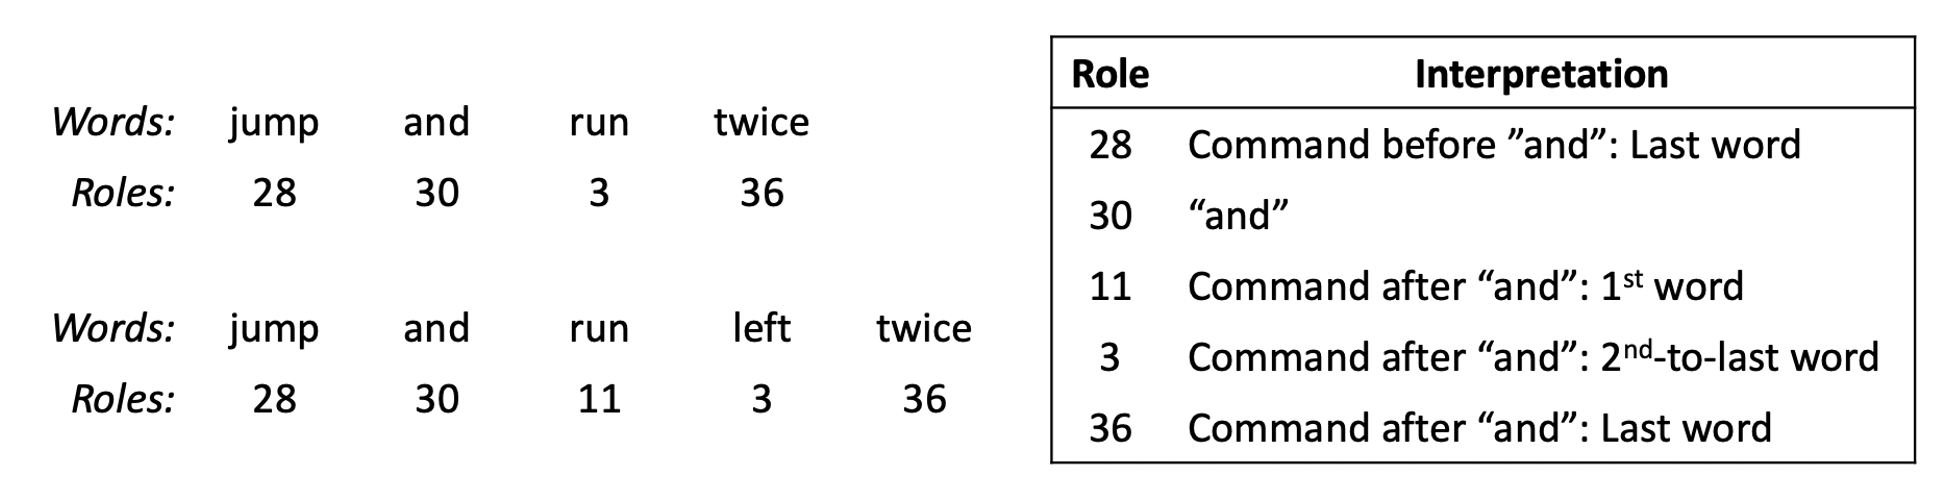
\includegraphics[width=.5\columnwidth]{images/rldn/rolefig2.png}
        
       \textbf{Step 2: Combine word and role vectors using a closed-form equation with learned parameters.} 
     %   {\scriptsize (\S \ref{sec:SCANnetReps})}
        
        \includegraphics[width=.5\columnwidth]{images/rldn/rolefig_middle.pdf}
        
         \end{tcolorbox}
        
        \hypersetup{linkcolor=blue}
        
        \begin{tcolorbox}[width=.5\columnwidth, colback={myblue}, coltitle=white, toptitle=3pt, bottomtitle=3pt, colframe={mybluebox},outer arc=2mm,colupper=black, valign=center, halign=left, boxsep = 0pt, title={\textbf{Results:}}, halign title=center, segmentation style={solid, line width=1pt}, left=3pt]
            \def\arraystretch{1.0}% 
            
        \textbf{The compositional encodings are functionally equivalent to the RNN encodings.} (\S \ref{sec:SCANnetReps})
    
        \includegraphics[width=.5\columnwidth]{images/rldn/rolefig_bottom1.pdf}
            
        \textbf{The RNN encodings can be manipulated in symbolic ways to alter the output.} (\S \ref{sec:Surgery})
        
        \includegraphics[width=.5\columnwidth]{images/rldn/rolefig_bottom2.pdf}
        
        \end{tcolorbox}
        
        \caption{Summary of our approach.}
        \label{fig:my_label}
    \end{figure}

Traditional models of cognition, and language in particular, have relied heavily on symbol structures and symbol manipulation.
However, in the current era, deep learning research has shown that Neural Networks (NNs) can display remarkable degrees of generalization on tasks traditionally viewed as depending on symbolic structure  \citep{googlenmt, mccoy}, albeit with some important limits to their generalization \citep{lake2018generalization}.
Given that standard NNs have no obvious mechanisms for representing symbolic structures, parsing inputs into such structures, nor applying compositional symbol-manipulating rules to them, this success raises the question that we address in this paper:\textbf{\emph{ How do NNs achieve such strong performance on compositional tasks?}} 

Could it be that NNs \textit{do} learn symbolic representations---covertly embedded as vectors in their state spaces?
\citet{mccoy} showed that 
when trained on highly compositional tasks, 
standard NNs learned representations that are functionally equivalent to compositional vector embeddings of symbolic structures (Sec. \ref{sec:TPR}). Processing in these NNs assigns structural representations to inputs and generates outputs that are governed by compositional rules stated over those representations. We refer to the networks we will analyze as \newterm{target NNs}, because we will propose a new type of NN (in Sec.~\ref{sec:Role-Learning})---the \newterm{Role Learner (\RLN)}---which is used to \textit{analyze} the target network.
%, after first discussing related analysis methods %of network analysis 
%in Sec.~\ref{sec:Related}.
In contrast with the analysis model of \citet{mccoy}, which relies on a hand-specified hypothesis about the structure underlying the learned representations of the target NN, \RLN\ \textit{automatically} learns a symbolic structure that best approximates the internal representation of the target network. This yields 
%Automating the discovery of structural hypotheses provides 
two %distinct 
advantages. 
First, \RLN\ achieves success at analyzing networks for which the underlying structure is unclear. We show this in Sec.~\ref{sec:SCAN}, where \RLN\ successfully uncovers the symbolic structures learned by a seq2seq RNN trained on the SCAN synthetic semantic parsing task \citep{lake2018generalization}. Second, removing the need for hand-specified structural hypotheses reduces the burden on the analyst, who only needs to provide input sequences and their target NN encodings. Discovering symbolic structure within a model enables us to perform precise alterations to the internal representations in order to produce desired alterations in the output (Sec.~\ref{sec:Surgery}). Then, in Sec.~\ref{sec:NLP}, we turn briefly to partially-compositional tasks in NLP.

The novel contributions of this research are:
\begin{itemize}
  \vspace{-2mm}
  \item ROLE, a NN module that learns to assign symbolic structures to input sequences (Sec.~\ref{sec:Role-Learning}).
  \vspace{-2mm}
  \item Demonstration that RNNs converge to compositional solutions on the synthetic SCAN task (Sec.~\ref{sec:SCAN}).
  \vspace{-2mm}
  \item A precise closed-form expression for the distributed encoding learned by an RNN trained on SCAN, exhibiting its latent symbolic structure (Sec.~\ref{sec:scan-role-interpretation}).
  \vspace{-2mm}
  \item Demonstration of the causal relevance of this symbolic structure by using the equation for its vector encoding to control RNN output through precise alteration of the RNN's internal encoding (Sec.~\ref{sec:Surgery}).
  \vspace{-2mm}
  \item Additional evidence showing that sentence embedding models do not capture compositional structure (Sec. \ref{sec:NLP}).
\end{itemize}

\section{Background Related work} \label{sec:Related}

\subsection{Compositionality}

Certain cognitive tasks consist in computing a function $\varphi$ that is governed by strict rules: e.g., if $\varphi$ is the function mapping a mathematical expression to its value (e.g., mapping `$19 - 2 * 7$' to $5$), then $\varphi$ obeys the rule that $\varphi(x + y) = \mathtt{sum}(\varphi(x), \varphi(y))$ for any expressions $x$ and $y$.
This rule is \newterm{compositional}: the output of a structure (here, $x + y$) is a function of the outputs of the structure's constituents (here, $x$ and $y$). The rule can be stated with full generality once the input is assigned a \newterm{symbolic structure} giving its decomposition into constituents. 
For a \newterm{fully-compositional} task, completely determined by compositional rules, a system that can assign appropriate symbolic structures to inputs and apply appropriate compositional rules to these structures will display full \newterm{systematic generalization}: it will correctly process arbitrary novel combinations of familiar constituents. This is a core capability of symbolic AI systems.

Other tasks, including most natural language tasks such as machine translation, are only partially characterizable by compositional rules: natural language is only partially compositional in nature. For example, if $\varphi$ is the function that assigns meanings to English adjectives, it generally obeys the rule that $\varphi(\mathtt{in\mbox{-}} + x) = \mathtt{not} \hs \varphi(x)$, (e.g., $\varphi(\mathtt{inoffensive}) = \mathtt{not} \hs \varphi(\mathtt{offensive})$), yet there are exceptions: $\varphi(\mathtt{inflammable}) = \varphi(\mathtt{flammable})$. On these ``\newterm{partially-compositional}'' tasks, this strategy of compositional analysis has demonstrated considerable, but limited, generalization capabilities.

\subsection{Analysis of NNs}

Many past works in the rich body of literature about analyzing NNs focus on compositional structure
%Our work falls within the larger paradigm of using analysis techniques to interpret NNs (see \citet{belinkov2019analysis} for a recent survey), often including a focus on compositional structure 
\citep{hupkes2020compositionality, hupkes2018visualisation, hewitt2019structural, li-etal-2019-compositional} and systematicity \citep{lake2018generalization,goodwin2020probing}. % NEW CONTENT (added "and systematicity")
Two of the most popular analysis techniques are the behavioral and probing approaches. In the behavioral approach, a model is evaluated  on a set of examples carefully chosen to require competence in particular linguistic phenomena \citep{marvin2018targeted, wang2018glue, dasgupta2019analyzing, poliak2018collecting,linzen2016assessing,mccoy2019right,warstadt2019blimp}. This technique can illuminate behavioral shortcomings but says little about how the internal representations are structured, treating the model as a black box.

In the probing approach, an auxiliary classifier is trained to classify the model's internal representations based on some linguistically-relevant distinction \citep{adi2016fine,giulianelli2018hood,conneau2018cram,conneau2018senteval,belinkov2017evaluating,blevins2018hierarchical,peters2018dissecting,tenney2018what}. In contrast with the behavioral approach, the probing approach tests whether some particular information is present in the model's encodings, but it says little about whether this information is actually used by the model. Indeed, in some cases models fail despite having the necessary information to succeed in their representations, showing that the ability of a classifier to extract that information does not mean that the model is using it \citep{ Voita2020InformationTheoreticPW, ravichander2020probing,vanmassenhove2017investigating}.

We build on \citet{mccoy}, which introduced the analysis task \newterm{DISCOVER (DISsecting COmpositionality in VEctor Representations)}:  take a NN and, to the extent possible, find an explicitly-compositional approximation to its internal distributed representations. DISCOVER allows us to bridge the gap between representation and behavior: It reveals not only what information is encoded in the representation, but also reveals this information in a way that we can manipulate to show that the information is causally implicated in the model's behavior (Section~\ref{sec:Surgery}). Moreover, it provides a much more comprehensive window into the representation than the probing approach does; while probing extracts particular types of information from a representation (e.g., ``does this representation distinguish between active and passive sentences?''), DISCOVER exhaustively decomposes the model's representational space. In this regard, DISCOVER is most closely related to the approaches of \citet{andreas2019measuring}, \citet{chrupala2019correlating}, and \citet{abnar2019blackbox}, who also propose methods for discovering a complete symbolic characterization of a set of vector representations, and \citet{omlin1996extraction} and \citet{weiss2018extracting}, which also seek to extract  more interpretable symbolic models that approximate neural network behavior.
Like \citet{andreas2019measuring} and \citet{chrupala2019correlating}, we seek to find the structure encoded in neural networks, rather than seeking structure directly from the data as is the goal in grammar induction work such as \citet{shen2018ordered} and \citet{bowman2016fast}.

\section{NN embedding of symbol structures} \label{sec:TPR}

\citeauthor{mccoy} showed that, in GRU \citep{cho-etal-2014-learning} encoder-decoder networks performing simple, fully-compositional string manipulations, the medial encoding (between encoder and decoder) could be extremely well approximated, up to an affine transformation, by \newterm{Tensor Product Representations (TPRs)} \citep{Smolensky:1990:TPV:102418.102425}, which are explicitly-compositional vector embeddings of symbolic structures. To represent a string of symbols as a TPR, the symbols in the string $\t{337}$ might be parsed into three constituents $\{ \t{3}\colon\!\r{pos}1, \t{7}\colon\!\r{pos}3, \t{3}\colon\!\r{pos}2 \}$, where $\r{pos}n$ is the role of $n^{\r{th}}$ position from the left edge of the string; other role schemes are also possible, such as roles denoting right-to-left position: $\{ \t{3}\colon\!\r{third\mbox{-}to\mbox{-}last}, \t{3}\colon\!\r{second\mbox{-}to\mbox{-}last}, \t{7}\colon\!\r{last} \}$. The embedding of a constituent $\t{7}\colon\!\r{pos}3$ is $\b{e}(\t{7}\colon\!\r{pos}3) = \b{e}_\rF(\t{7}) \otimes \b{e}_\rR(\r{pos3})$, where $\otimes$ is the tensor product (outer product), $\b{e}_\rR, \b{e}_\rF$ are respectively a vector embedding of the roles and a vector embedding of the \newterm{fillers} of those roles: the digits. The embedding of the whole string is the sum of the embeddings of its constituents. 
In general, for a symbol structure $\t{S}$ with roles $\{ r_k \}$ that are respectively filled by the symbols $\{ \t{f}_k \}$,
$\b{e}_\r{TPR}(\t{S}) = \sum_k \b{e}_\rF(\t{f}_k) \otimes \b{e}_\rR(r_k)$. The DISCOVER task including the TPR equations is depicted in Figure \ref{fig:discover}.

\begin{figure}[t]
    \centering
    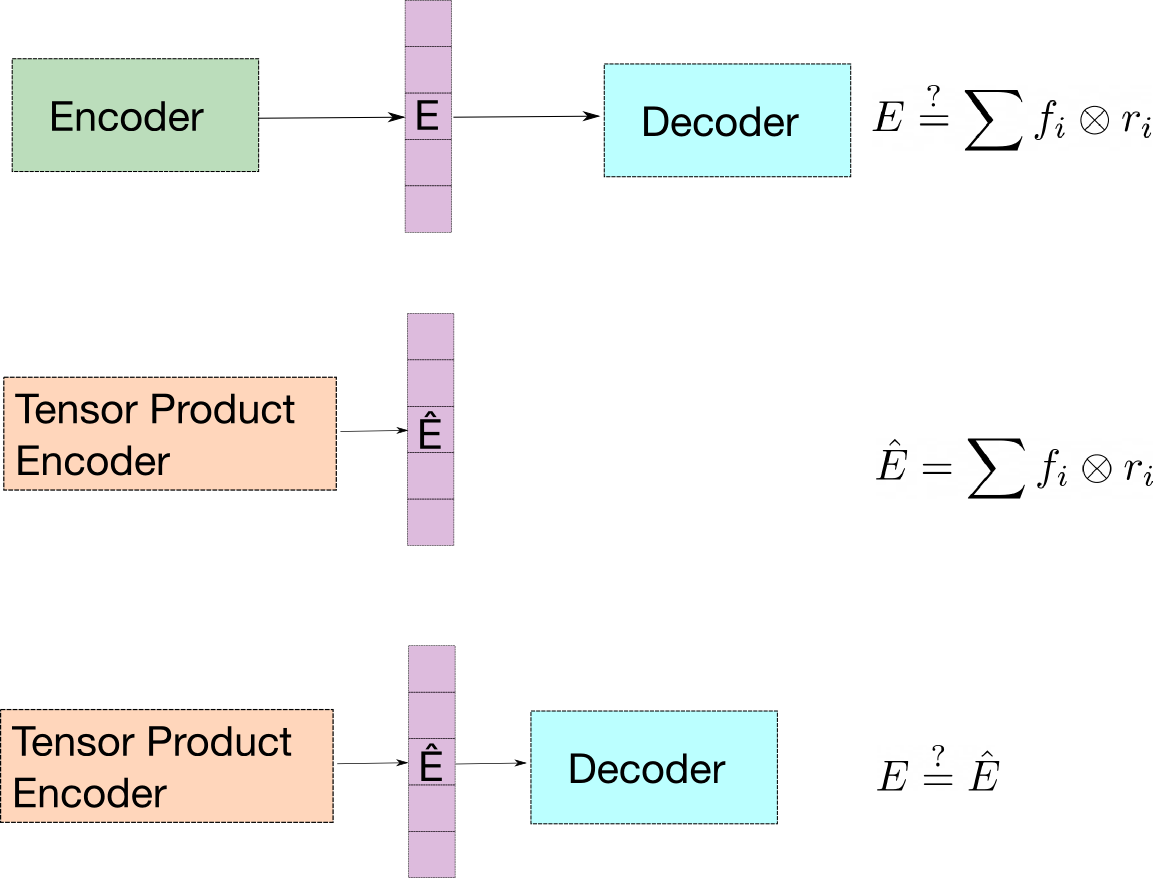
\includegraphics[scale=.25]{images/rldn/task.png}
    \caption{The DISCOVER task and functions. At the top is the target network and question we pose: is the internal embedding a TPR? The middle row is the TPE which follows the provided equation. We train the TPE to minimize the MSE between $\hat{E}$ and $E$. In the bottom row, we evaluate our model by passing the approximations $\hat{E}$ through the decoder and checking the \textit{substitution accuracy} --- the proportion of examples for which the approximated encoding $\hat{E}$ yields the correct output when provided to the decoder .}
    \label{fig:discover}
\end{figure}

At a high level, these role embeddings serve a similar purpose as positional embeddings in a Transformer \citep{vaswani2017attention}, in that they are vector embeddings of a token's position in a sequence. The roles discussed above---and the positional embeddings used in Transformers---illustrate \textbf{role schemes} based on sequential position; non-sequential role schemes such as positions in a tree are also possible. \citet{mccoy} showed that,for a given seq2seq architecture learning a given string-mapping task, there exists a highly accurate TPR approximation of the medial encoding, given an appropriate  pre-defined role scheme. The main technical contribution of the present paper is the Role Learner (ROLE) model, an RNN that learns its own role scheme to optimize the fit of a TPR approximation to a given set of internal representations in a pre-trained target NN. This makes the DISCOVER framework more general by removing the need for human-generated hypotheses about the role schemes the network might be implementing. Learned role schemes, we will see in Sec.~\ref{sec:SCANnetReps}, can enable good TPR approximation of networks for which human-generated role schemes fail.

\section{The Role Learner (ROLE) Model} \label{sec:Role-Learning} 

\RLN\footnote{Code available at \url{https://github.com/psoulos/role-decomposition}.} produces a vector-space embedding of an input string of $T$ symbols $\t{S} = \t{s}_1 \t{s}_2 \ldots \t{s}_T$ by producing a TPR $\b{T}(\t{S})$ and then passing it through an affine transformation.
%$\bW$.
\RLN\ is trained to approximate a pre-trained target string-encoder $\c{E}$.
Given a set of $N$ training strings $\{ \t{S}^{(1)}, \ldots, \t{S}^{(N)} \}$, \RLN\ minimizes the total mean-squared error (MSE) between its output $\bW\,\b{T}(\t{S}^{(i)}) + \vb$ and %$\c{E}$'s corresponding output, 
$\c{E}(\t{S}^{(i)})$.

\begin{figure}[t]
    \centering
    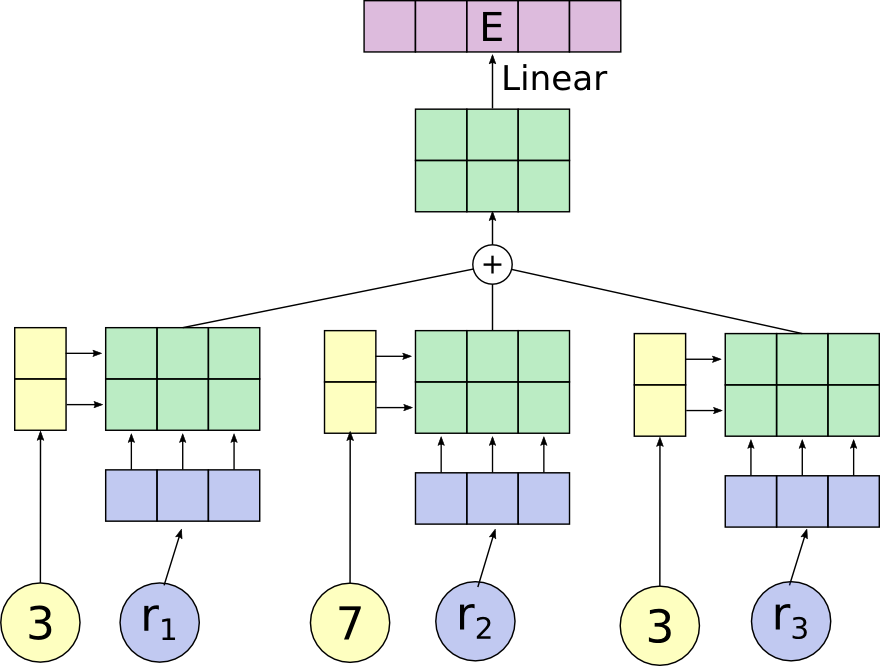
\includegraphics[scale=.3]{images/rldn/tpdn.png}
    \caption{The Tensor Product Encoder architecture. The fillers (yellow circles) and roles (blue circles) are first vectorized with an embedding layer. These two vector embeddings are combined by an outer product to produce the green matrix representing the TPR of the constituent. All of the constituents are summed together to produce the TPR of the sequence, and then a linear transformation is applied to resize the TPR to the target encoder's dimensionality. \RLN\ replaces the role embedding layer and directly produces the blue role vector.}
    \label{fig:tpe-arch}
\end{figure}

\RLN\ is an extension of the Tensor-Product Encoder (TPE) introduced in \citet{mccoy} (as the ``Tensor Product Decomposition Network'') and depicted in Figure \ref{fig:tpe-arch}. 
Crucially, \RLN\ is not \textit{given} role labels for the input symbols, but \textit{learns to compute} them.
More precisely, it learns a dictionary of $n_\rR$ $d_\rR$-dimensional role-embedding vectors, 
$\mR \in \R^{d_\rR \times n_\rR}$, and, for each input symbol 
$\t{s}_t$, computes a soft-attention vector $\va_t$ over these role vectors: 
the role vector assigned to $\t{s}_t$ is then the attention-weighted linear combination of role vectors, $\vr_t = \mR\, \va_t$. \RLN\ simultaneously learns a dictionary of $n_\rF$ $d_\rF$-dimensional symbol-embedding filler vectors $\mF \in \R^{d_\rF \times n_\rF}$, the $\phi^{\r{th}}$ column of which is $\vf_\phi$, the embedding of symbol type $\phi$; $\phi \in 1, \ldots, n_\rF$ where $n_\rF$ is the size of the vocabulary of symbol types.
The TPR generated by \RLN\ is thus $\b{T}(\t{S}) = \sum_{t=1}^T \vf_{\tau(\t{s}_t)} \otimes \vr_t$, where $\tau(\t{s}_t)$ is symbol $\t{s}_t$'s type.
Finally, \RLN\ learns an affine transformation to map this TPR into $\R^d$, where $d$ is the dimension of the representations of the encoder $\c{E}$.
%it is learning to approximate.

\begin{figure}[t]
    \captionsetup{width=\columnwidth}
    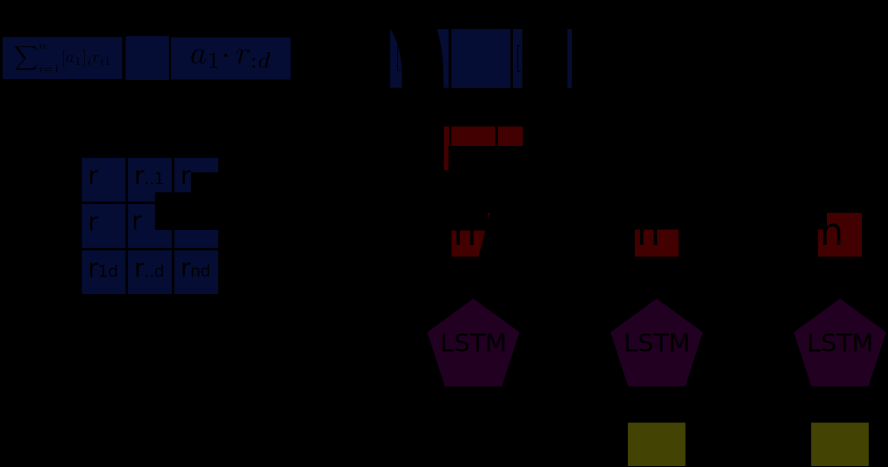
\includegraphics[width=\columnwidth]{images/rldn/role_assigner_shrink}
    \caption{The role learning module. The role attention vector $a_t$ is encouraged to be one-hot through regularization; if $a_t$ were one-hot, the produced role embedding $r_t$ would correspond directly to one of the roles defined in the role matrix $\mR$. The LSTM can be unidirectional or bidirectional.}
    \label{fig:role_learner}
\end{figure}

\RLN\ uses an LSTM \citep{Hochreiter:1997:LSM:1246443.1246450} to compute the role-assigning attention-vectors $\va_t$ from its learned embedding $\mF$ of the input symbols $\t{s}_t$: at each $t$, the hidden state of the LSTM passes through a linear layer and then a softmax to produce $\va_t$ (depicted in Figure \ref{fig:role_learner}). Let the $t^{\r{th}}$ LSTM hidden state be $\vq_t \in \R^H$; let the output-layer weight-matrix have rows $\vk_\rho^\top \in \R^H$ and let the columns of $\mR$ be $\vv_\rho \in R^{d_\rR}$, with $\rho = 1,\dots,n_\rR$. Then $\vr_t = \mR\, \va_t = \sum_{\rho=1}^{n_\rR} \vv_\rho\, \softmax ( \vk_\rho^\top \vq_t )$: the result of query-key attention  \citep[e.g.,][]{vaswani2017attention} with query $\vq_t$ to a fixed external memory containing key-value pairs $\{ ( \vk_\rho, \vv_\rho ) \}_{\rho=1}^{n_\rR}$.

Since a TPR for a discrete symbol structure deploys a discrete set of roles specifying discrete structural positions, ideally a single role would be selected for each $\t{s}_t$: $\va_t$ would be one-hot.
\RLN\ training therefore deploys regularization to bias learning towards one-hot $\va_t$ vectors (based on the regularization proposed in \citet{palangi}, developed for the same purpose). See Appendix \ref{sec:role-regulatization} for the precise regularization terms that we used.

It is essential to note that, while we impose this regularization on \RLN, there is no explicit bias favoring discrete compositional representations in the \textit{target encoder} $\c{E}$: any such structure that \RLN\ finds hidden in the representations learned by $\c{E}$ must result from biases implicit in the vanilla RNN-architecture of $\c{E}$ when applied to its target task.

\section{The SCAN task} \label{sec:SCAN}

Returning to our central question from Sec.~\ref{sec:Intro}, how can neural networks \textit{without} explicit compositional structure perform well on fully-compositional tasks? 
Our hypothesis is that, though these models have no \textit{constraint} forcing them to be compositional, they still have the \textit{ability} to implicitly learn compositional structure.
To test this hypothesis, we apply \RLN\ to a standard RNN-based seq2seq model \citep{sutskever2014sequence} trained on a fully compositional task. Because the RNN has no constraint forcing it to use TPRs, we do not know \textit{a priori} whether there exists any solution that \RLN\ could learn; thus, if \RLN\ does learn anything it will be a significant empirical finding about how these RNNs operate.

We consider the SCAN task \citep{lake2018generalization}, which was designed to test compositional generalization and systematicity. SCAN is a synthetic semantic parsing
%sequence-to-sequence mapping 
task: an input sequence describing an action plan, e.g., \textcolor{violet}{$\t{jump \hs opposite \hs left}$}, is mapped to a sequence of primitive actions, e.g., \textcolor{violet}{$\t{TL \hs TL \hs JUMP}$} (see Sec.~\ref{sec:Surgery} for a complex example). We use \textcolor{violet}{$\t{TL}$} to abbreviate \textcolor{violet}{$\t{TURN\_LEFT}$}, sometimes written \textcolor{violet}{$\t{LTURN}$}; similarly, we use \textcolor{violet}{$\t{TR}$} for \textcolor{violet}{$\t{TURN\_RIGHT}$}. The SCAN mapping is defined by a complete set of compositional rules \citep[Supplementary Fig. 7]{lake2018generalization}. 

\begin{table*}[ht]
\resizebox{\textwidth}{!}{
\begin{tabular}{ c c c c c c c c c} 
 \toprule
  \textbf{Continuous} & \textbf{Snapped} & \textbf{Discrete} & LTR & RTL & Bi & Tree & Wickel & BOW \\ 
  \midrule
  94.83\% & 81.71\% $\pm$ 7.28 & 92.44\% & 6.68\% & 6.96\% & 10.72\% & 4.31\% & 44.00\% & 4.52\% \\
 \bottomrule
\end{tabular}
}
\caption{\label{tab:scan-accuracy}Mean substitution accuracy for learned (bold) and hand-defined role schemes on SCAN across three random initializations. Standard deviation was below 1\% for all schemes except for snapped. Substitution accuracy is measured by feeding \RLN's approximation to the target decoder. (Sec.~\ref{sec:SCANnetReps})}
\end{table*}

\subsection{The compositional structure of SCAN encoder representations} \label{sec:SCANnetReps}

For our target SCAN encoder $\c{E}$, we trained a standard GRU with one hidden layer of dimension 100 for 100,000 steps (batch-size 1) with a dropout of 0.1 on the simple train-test split (hyperparameters determined by a limited search; see Appendix \ref{sec:rnn-scan}).
$\c{E}$ achieves $98.47\%$ (full-string) accuracy on the test set. Thus $\c{E}$ provides what we want: a standard RNN achieving near-perfect accuracy on a non-trivial fully compositional task.

After training, we extract the final hidden embedding from the encoder for each example in the training and test sets. These are the encodings we attempt to approximate as explicitly compositional TPRs. 
We provide \RLN\ with 50 roles to use as it wants (hyperparameters described in Appendix \ref{sec:role-scan}).
We evaluate the substitution accuracy that this learned role scheme provides in three ways. The \newterm{continuous} method tests ROLE in the same way as it was trained, with input symbol $\t{s}_t$ assigned role vector $\vr_t = \mR\, \va_t$. The continuous method does not produce a discrete set of role vectors because the linear layer that generates $a_t$ allows for continuously-valued weights. The remaining two methods test the efficacy of a truly discrete set of role vectors. First, in the \newterm{snapped} method, $\va_t$ is replaced at evaluation time by the one-hot vector $\vm_t$ singling out role $m_t = \argmax(\va_t)$: $\vr_t = \mR\, \vm_t$. This method serves the goal of enforcing the discreteness of roles, but it is expected to decrease performance because it tests ROLE in a different way than it was trained. Our final evaluation method, the \newterm{discrete} method, uses discrete roles without having such a train/test discrepancy by using a two-stage process. In the first stage, the snapped method is used to output one-hot vector roles $\vm_t$ for every symbol in the dataset. In the second stage, we train a TPE which does not learn roles but rather uses the one-hot vector $\vm_t$ as input during training. In this case, \RLN\ acts as an automatic data labeler, assigning a role to every input word.

For comparison, we also train TPEs using a variety of discrete hand-crafted role schemes: left-to-right (LTR), right-to-left (RTL), bidirectional (Bi), tree position, neighbor-based Wickelrole (Wickel), and bag-of-words (BOW) (descriptions of these role schemes are in Appendix \ref{sec:role-schemes}). 

The mean substitution accuracy from these different methods is shown in Table \ref{tab:scan-accuracy}. 
All of the predefined role schemes provide poor approximations, none surpassing $44.00\%$ accuracy. 
The role scheme learned by \RLN\ does significantly better than any of the predefined role schemes: when tested with the basic, continuous role-attention method, the accuracy is $94.83\%$. 

The success of \RLN\ 
tells us two things. First, it shows that the target model's compositional behavior relies on compositional internal representations: it was by no means guaranteed to be the case that \RLN\ would be successful here, so the fact that it is successful tells us that the encoder has learned compositional representations. Second, it adds further validation to the efficacy of \RLN, because it shows that it can be a useful analysis tool in cases of significantly greater complexity than the simple string manipulation tasks studied in \citet{mccoy}. 
In fact, it allows us to \textit{\textbf{write in closed form the embedding}} $\b{e}(\t{S})$ of an input $\t{S} = \t{s}_1\ldots\t{s}_T$ that is learned by the SCAN encoder, to an excellent degree of approximation (as measured by substitution accuracy):
$\b{e}(\t{S}) = \bW \sum_{t=1}^T \vf_{\tau(\t{s}_t)} \otimes \vr_{\rho(\t{s}_t)} + \vb$, where $\tau(\t{s}_t)$ is symbol $\t{s}_t$'s type, $\rho(\t{s}_t)$ is the role assigned to $\t{s}_t$ by the algorithm discussed next,
%given in \hl{Appendix} \ref{sec:Alg}, 
and the matrices $\bW$, $\mF = [\vf_1 \ldots \vf_{n_\rF} ]$, and $\mR = [\vr_1 \ldots \vr_{n_\rR}]$ and bias vector $\vb$ are learned by \RLN.
Note that this expression is bilinear, even though the GRU encoder that generates it includes nonlinearities.

\subsection{Interpreting the learned role scheme}\label{sec:scan-role-interpretation}

By analyzing the roles assigned by ROLE to the sequences in the SCAN training set, we created a symbolic algorithm for predicting which role will be assigned to each filler. This section covers the primary factors of the algorithm, while the entire algorithm is described in Appendix \ref{sec:Alg} and discussed at additional length in Appendix \ref{sec:AlgDisc}. Though the algorithm was created based only on sequences in the SCAN training set, it is equally successful at predicting which roles will be assigned to test sequences, exactly matching \RLN's predicted roles for 98.7\% of sequences.

%The details of this algorithm illuminate 
The algorithm illuminates how the filler-role scheme encodes information relevant to the task. First, one of the initial facts that the decoder must determine is whether the sequence is a single command, a pair of subcommands connected by \textcolor{violet}{$\t{and}$}, or a pair of subcommands connected by \textcolor{violet}{$\t{after}$}; such a determination is crucial for knowing the basic structure of the output (how many actions to perform and in what order). We have found that role 30 is used for, and only for, the filler \textcolor{violet}{$\t{and}$}, while role 17 is used in and only in sequences containing \textcolor{violet}{$\t{after}$} (usually with \textcolor{violet}{$\t{after}$} as the filler bound to role 17). Thus, the decoder can use these roles to tell which basic structure is in play: if role 30 is present, it is an \textcolor{violet}{$\t{and}$} sequence; if role 17 is present, it is an \textcolor{violet}{$\t{after}$} sequence; otherwise it is a single command.

Once the decoder has established the basic syntactic structure of the output, it must then fill in the particular actions. This can be accomplished using the remaining roles, which mainly encode absolute position within a subcommand. For example, the last word of a subcommand before \textcolor{violet}{$\t{after}$} (e.g., \textcolor{violet}{$\t{jump \hs \textbf{left} \hs after \hs walk \hs twice}$}) is always assigned role 8, while the last word of a subcommand after \textcolor{violet}{$\t{after}$} (e.g., \textcolor{violet}{$\t{jump \hs left \hs after \hs walk \hs \textbf{twice}}$}) is always assigned role 46. Therefore, once the decoder knows (based on the presence of role 17) that it is dealing with an \textcolor{violet}{$\t{after}$} sequence, it can check for the fillers bound to roles 8 and 46 to begin to figure out what the two subcommands surrounding \textcolor{violet}{$\t{after}$} look like. The identity of the last word in a subcommand is informative because that is where a cardinality (i.e., \textcolor{violet}{$\t{twice}$} or \textcolor{violet}{$\t{thrice}$}) appears if there is one. Thus, by checking what filler is at the end of a subcommand, the model can determine whether there is a cardinality present and, if so, which one.

ROLE itself does not provide an interpretation for the symbolic structure it generates, but
we have shown that this structure can be successfully interpreted by humans. By contrast, it is very difficult to interpret the continuous neuron values of RNN representations; even the rare successful cases of doing so, such as \citet{lakretz2019emergence} and \citet{mu2020compositional}, only interpret a few isolated units, while we were able to exhaustively explain the entire symbolic structure discovered by ROLE.


\begin{figure*}[ht]
    \begin{center}
    \begin{subfigure}{0.5\textwidth}
    \fontsize{7}{8}\selectfont
    $   
    \t{run}\colon\!11 \hs \t{left}\colon\!36 \hs \t{twice}\colon\!8 \hs \t{after}\colon\!43 \hs \t{jump}\colon\!10 \hs \t{opposite}\colon\!17 \hs \t{right}\colon\!4 \hs \t{thrice}\colon\!46 \rightarrow \t{\hs\hs\hs\hs\hs\hs\hs\hs}\t{TR \hs TR \hs JUMP \hs TR \hs TR \hs JUMP \hs TR \hs TR \hs JUMP \hs TL \hs RUN \hs TL \hs RUN} \leavevmode\newline -\t{run}\colon\!11 \hs +\t{look}\colon\!11 \rightarrow \leavevmode\newline \t{\hs\hs\hs\hs\hs\hs\hs\hs}\t{TR \hs TR \hs JUMP \hs TR \hs TR \hs JUMP \hs TR \hs TR \hs JUMP \hs TL \hs \hi{LOOK} \hs TL \hs \hi{LOOK}} \leavevmode\newline
    -\t{jump}\colon\!10 \hs +\t{walk}\colon\!10 \rightarrow\leavevmode\newline
    \t{\hs\hs\hs\hs\hs\hs\hs\hs}\t{TR \hs TR \hs \hi{WALK} \hs TR \hs TR \hs \hi{WALK} \hs TR \hs TR \hs \hi{WALK} \hs TL \hs LOOK \hs TL \hs LOOK} \leavevmode\newline
    -\t{left}\colon\!36 \hs +\t{right}\colon\!36 \rightarrow\leavevmode\newline
    \t{\hs\hs\hs\hs\hs\hs\hs\hs}\t{TR \hs TR \hs WALK \hs TR \hs TR \hs WALK \hs TR \hs TR \hs WALK \hs \hi{TR} \hs LOOK \hs \hi{TR} \hs LOOK} \leavevmode\newline
    -\t{twice}\colon\!8 \hs +\t{thrice}\colon\!8 \rightarrow\leavevmode\newline
    \t{\hs\hs\hs\hs\hs\hs\hs\hs}\t{TR \hs TR \hs WALK \hs TR \hs TR \hs WALK \hs TR \hs TR \hs WALK \hs TR \hs LOOK \hs } \leavevmode\newline
    \t{\hs\hs\hs\hs\hs\hs\hs\hs}\t{TR \hs LOOK \hs \hi{TR \hs LOOK}} \leavevmode\newline
    -\t{opposite}\colon\!17 \hs +\t{around}\colon\!17 \rightarrow\leavevmode\newline
    \t{\hs\hs\hs\hs\hs\hs\hs\hs}\hi{\t{TR \hs WALK \hs TR \hs WALK \hs TR \hs WALK \hs TR \hs WALK \hs TR \hs WALK \hs TR \hs WALK}} \leavevmode\newline
    \t{\hs\hs\hs\hs\hs\hs\hs\hs}\hi{\t{TR \hs WALK \hs TR \hs WALK \hs TR \hs WALK \hs TR \hs WALK \hs \hi{TR \hs WALK \hs TR \hs WALK} \hs }} \leavevmode\newline
    \t{\hs\hs\hs\hs\hs\hs\hs\hs}\t{TR \hs LOOK \hs TR \hs LOOK \hs TR \hs LOOK} \leavevmode\newline
$
        \label{fig:role-distribution}
    \end{subfigure}
    \hfill
    \begin{subfigure}{0.28\textwidth}
        \hspace{-40pt}
        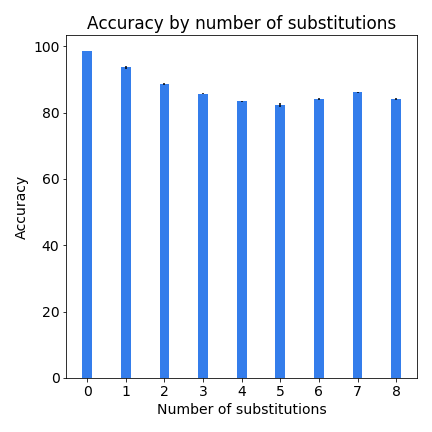
\includegraphics[width=\textwidth]{images/rldn/sub-accuracy.png}
        \label{fig:surgery}
    \end{subfigure}
    \caption{Left: Example of successive constituent surgeries. The roles assigned to the input symbols are indicated in the first line (e.g., \textcolor{violet}{$\t{run}$} was assigned role $11$). Altered output symbols are in blue. The model produces the correct outputs for all cases shown here. Right: Mean constituent-surgery accuracy across three runs. Standard deviation is below 1\% for each number of substitutions. (Sec.~\ref{sec:Surgery})}
    \label{fig:Figs12}
    \end{center}
\end{figure*}

\subsection{Precision constituent-surgery on internal representations produces desired outputs} \label{sec:Surgery}

The substitution-accuracy results above show that if the \textit{entire} learned representation is replaced by \RLN's approximation, the output remains correct. But do the \textit{individual word embeddings} in this TPR have the appropriate causal consequences when processed by the decoder?%\footnote{Historically, this question has had considerable significance: the original compositionality challenge to neural network models of cognition by Fodor and colleagues \citep{fodor1988connectionism} insisted that constituents of cognitive representations must individually be \textit{causally efficacious} in order for those constituents to provide an explanation of the compositionality of cognition \citep{fodor1990connectionism, fodor1997connectionism}. That TPRs meet the challenge of explaining compositionality was argued in \citet{smolensky1987constituent,smolensky1991connectionism}.}

To address this causal question \citep{pearl2000causality}, we actively intervene on the constituent structure of the internal representations by replacing one constituent with another syntactically equivalent
one,\footnote{We extract syntactic categories from the SCAN grammar \citep[Supplementary Fig. 6]{lake2018generalization} by saying that two words belong to the same category if every occurrence of one could be grammatically replaced by the other. We do not replace occurrences of \textcolor{violet}{$\t{and}$} and \textcolor{violet}{$\t{after}$} since the presence of either of these words causes substantial changes in the roles assigned within the sequence (Appendix \ref{sec:Alg}).} and see whether this produces the expected change in the output of the decoder.
We take the encoding generated by the RNN encoder $\c{E}$ for an input such as \textcolor{violet}{$\t{jump \hs opposite \hs left}$}, subtract the vector embedding of the \textcolor{violet}{$\t{opposite}$} constituent, add the embedding of the \textcolor{violet}{$\t{around}$} constituent, and see whether this causes the output to change from the correct output for \textcolor{violet}{$\t{jump \hs opposite \hs left}$ ($\t{TL \hs TL \hs JUMP)}$} to the correct output for \textcolor{violet}{$\t{jump \hs around \hs left}$ ($\t{TL \hs JUMP \hs TL \hs JUMP \hs TL \hs JUMP \hs TL \hs JUMP}$)}. The roles in these constituents are determined by the algorithm of Appendix \ref{sec:Alg}. If changing a word leads other roles in the sequence to change (according to the algorithm), we update the encoding with those new roles as well. Such surgery can be viewed as a more general extension of the analogy approach used by \citet{mikolov2013linguistic} for analysis of word embeddings.
An example of applying a sequence of five such constituent surgeries to a sequence is shown in Figure~\ref{fig:Figs12} (left). Even long sequences of such replacements produce the expected change in the decoder's output with high accuracy (Figure~\ref{fig:Figs12}, right), indicating that the compositional structure discovered by ROLE does play a central causal role in the model's behavior.

\section{Partially-compositional NLP tasks} \label{sec:NLP}
The previous sections explored fully-compositional tasks where there is a strong signal for compositionality. In this section, we explore whether the representations of NNs trained on tasks that are only partially-compositional also capture compositional structure. Partially-compositional tasks are especially challenging to model because a fully-compositional model may enforce compositionality too strictly to handle the non-compositional aspects of the task, while a model without a compositional bias may not learn any sort of compositionality from the weak cues in the training set.

We test four sentence encoding models for compositionality: InferSent \citep{conneau2017supervised}, Skip-thought \citep{kiros2015skip}, Stanford Sentiment Model (SST) \citep{socher2013recursive}, and SPINN \citep{bowman2016fast}. For each of these models, we extract the encodings for the SNLI premise sentences \citep{bowman2015large}. We use the extracted embeddings to train \RLN\ with 50 roles available (additional training information provided in Appendix \ref{sec:role-sentences}).

\begin{table*}[h!]
    \centering
   \resizebox{\textwidth}{!}{
		\begin{tabular} {lcccccccc}
			\toprule
		 & \textbf{Continuous} & \textbf{Snapped} & \textbf{Discrete} & LTR & RTL & Bi & Tree & BOW \\ \midrule
		InferSent & \textbf{4.05e-4} & 4.15e-4 & 5.76e-4 & 8.21e-4 & 9.70e-4 & 9.16e-4 & 7.78e-4 & 4.34e-4 \\
		Skip-thought & 9.30e-5 & 9.32e-5 & 9.85e-5 & 9.91e-5 & 1.78e-3 & 3.95e-4 & 9.64e-5 & \textbf{8.87e-5} \\
		SST & \textbf{5.58e-3} & 6.72e-3 & 6.48e-3 & 8.35e-3 & 9.29e-3 & 8.55e-3 & 5.99e-3 & 9.38e-3 \\
		SPINN & \textbf{.139} & .151 & .147 & .184 & .189 & .181 & .178 & .176 \\ \bottomrule
		\end{tabular}
		}
    \caption{\label{tab:sent-emb-mse}MSE loss for learned (bold) and hand-crafted role schemes on sentence embedding models. (Sec.~\ref{sec:NLP})}

\end{table*}

As a baseline, we also train TPEs that use pre-defined role schemes (hyperparameters described in Appendix \ref{sec:tpe-sentences}). For all of the sentence embedding models except Skip-thought, \RLN\ with continuous attention provides the lowest mean squared error at approximating the encoding (Table~\ref{tab:sent-emb-mse}). The BOW (bag-of-words) role scheme represents a TPE that uses a degenerate `compositional' structure which assigns the same role to every filler; for each of the sentence embedding models tested except for SST, performance is  within the same order of magnitude as structure-free BOW. \citet{parikh2016decomposable} found that a bag-of-words model scores extremely well on Natural Language Inference despite having no knowledge of word order, showing that structure is not necessary to perform well on the sorts of tasks commonly used to train sentence encoders. Although not definitive, the \RLN\ results provide no evidence that these models' sentence embeddings possess compositional structure.

In future work, it would be interesting to perform a similar analysis on Transformer architectures \citep{vaswani2017attention}. Such models have displayed impressive syntactic generalization \cite{hu2020systematic} and few-shot learning of compositional tasks \cite{brown2020language}, both of which suggest that they learn substantial degrees of compositional structure; thus, ROLE may be more likely to discover meaningful structure in Transformers than in the sentence-embedding models in Table \ref{tab:sent-emb-mse}. Further work has found impressive degrees of syntactic structure in Transformer encodings \cite{hewitt2019structural}, suggesting that there may well be compositional structure for ROLE to pick up on. The main difficulty in applying ROLE to Transformers---and the reason we did not include Transformers in our study---is that the sentence representation used by a Transformer is typically viewed as a variable-sized collection of vectors, whereas ROLE requires single-vector representations; this discrepancy must be overcome if ROLE is to be applied to Transformers. 

One past work \cite{jawahar-etal-2019-bert} has applied ROLE's precursor (the TPDN of \citet{mccoy}) to Transformer representations by choosing the [CLS] token of BERT \cite{devlin2019bert} as the single-vector sentence encoding to decompose. \citeauthor{jawahar-etal-2019-bert} found that these encodings were approximated better by human-specified tree-position roles than by other human-specified candidates (e.g., left-to-right and right-to-left roles). By removing the constraint of requiring human-designed role schemes, ROLE may be able to discover other role schemes that approximate BERT's encodings even more closely.
% The main difficulty in applying ROLE to Transformers---and the reason we did not include Transformers in our study---is that the sentence representation used by a Transformer is typically viewed as a variable-sized collection of vectors, whereas ROLE requires single-vector representations; this discrepancy must be overcome if ROLE is to be applied to Transformers.

\section{Conclusion} \label{sec:Conclusion}

We have introduced \RLN, a neural network that learns to approximate the representations of an existing target neural network $\c{E}$ using an explicit symbolic structure. \RLN\ successfully discovers symbolic structure in a standard RNN trained on the fully-compositional SCAN semantic parsing task, even though the RNN has no such structure explicitly present in its architecture. This yields a closed-form equation for the RNN's encoding of any input string. 
When applied to sentence embedding models trained on partially-compositional tasks, \RLN\ performs better than hand-specified hypothesized structures but still provides little evidence that the sentence encodings represent compositional structure. 

While this work has shown that NNs can converge to TPRs to solve compositional tasks, it is still unknown how the weights in the NN actually convert the raw input into a TPR. To investigate this process, in future work we plan to apply our technique to representations of partial sequences. For instance, when the complete input is \textcolor{violet}{$\t{jump \hs right \hs twice}$}, the target RNN must first represent \textcolor{violet}{$\t{jump \hs right}$} as a well-formed TPR at the point when only those two words have been encountered. The representation then needs to be updated when the next word, \textcolor{violet}{$\t{twice}$}, is encountered. By studying the nature of that update, we can gain insight into how the target model builds up a TPR from the input elements.



Uncovering the latent symbolic structure of NN representations learned for fully-compositional tasks is a significant step towards explaining how NNs achieve the level of compositional generalization that they do. In addition, by illuminating shortcomings in the representations learned for standard tasks that are not fully-compositional, ROLE can help suggest types of inductive bias for improving models' generalization with standard, partially-compositional datasets.
\newcommand{\blackboard}[0]{\emph{DTM}}
\newcommand{\car}{\texttt{car}}
\newcommand{\cdr}{\texttt{cdr}}
\newcommand{\cons}{\texttt{cons}}
\chapter{Differentiable Tree Operations Promote Compositional Generalization} \label{chap:chap-2}

%%%% MUST: if the chapter is a reprint or submitted paper, you must declare it
%% you can use enumerate or itemize environment if you have more than one paper 
%% \mybibexclude{} will exclude this citation from the final bibliography
%% if this paper appears somewhere else then remove \mybibexclude{} command

\begin{singlespace}         % you can also use `onehalfspace` to relax the spacing
    This chapter is reprinted from \fullcite{pmlr-v202-soulos23a}. Licensed under CC BY 4.0.
\end{singlespace} 

%%%% remove the following and add your chapter text here
\begin{abstract}
    In the context of structure-to-structure transformation tasks, learning sequences of discrete symbolic operations poses significant challenges due to their non-differentiability. To facilitate the learning of these symbolic sequences, we introduce a differentiable tree interpreter that compiles high-level symbolic tree operations into subsymbolic matrix operations on tensors. We present a novel Differentiable Tree Machine (\blackboard) architecture that integrates our interpreter with an external memory and an agent that learns to sequentially select tree operations to execute the target transformation in an end-to-end manner. With respect to out-of-distribution compositional generalization on synthetic semantic parsing and language generation tasks, \blackboard\ achieves 100\% while existing baselines such as Transformer, Tree Transformer, LSTM, and Tree2Tree LSTM achieve less than 30\%. \blackboard\ remains highly interpretable in addition to its perfect performance.
\end{abstract}

\section{Introduction}
\begin{figure}[ht]
\vskip 0.2in
\begin{center}
\centerline{\includegraphics[width=1.0\columnwidth]{images/dtm/overview.pdf}}
\caption{A high level overview of our model which consists of three modules. The Neural Tree Agent is a learnable component which, at each step of processing, selects the operation to perform and the arguments over which to operate. The Differentiable Tree Interpreter is a closed-form function precomputed at initialization which compiles high level symbolic operations into subsymbolic matrix operations on tensors. The output of the interpreter is a blended tree that is written to Tree Memory, which functions as a working memory to hold various partial and candidate trees. The final tree written to memory is the output tree. Blue represents the component with learnable parameters, and green represents components that operate in tree space. }
\label{fig:high-level}
\end{center}
\vskip -0.2in
\end{figure}

Symbolic manipulation is a hallmark of human reasoning \citep{Newell1980PhysicalSS, newell1982knowledge}. Reasoning within the symbolic space through discrete symbolic operations can lead to improved out-of-distribution (OOD) generalization and enhanced interpretability. Despite the significant advances in representation learning made by modern deep learning, learning to directly manipulate discrete symbolic structures remains a challenge. One key issue is the non-differentiability of discrete symbolic operations, which makes them incompatible with gradient-based learning methods. Continuous representations offer greater learning capacity, but often at the expense of interpretability and compositional generalization.

Tensor Product Representation (TPR) provides a general encoding of structured symbolic objects in vector space \cite{Smolensky1990TensorPV}. TPR decomposes a symbolic object into a set of role-filler pairs, such as a position in a tree (the role) and the label for that position (the filler of that role). The role and filler in each pair are represented by vectors and bound together using the tensor product operation.

In this work, we focus on binary trees and three Lisp operators: \car, \cdr, and \cons\ \cite{steele1990common} (also known as left-child, right-child, and construct new tree). Examples of these operations are shown in Figure \ref{fig:car-cdr-cons}. Crucially, within the TPR space, these symbolic operators on discrete objects become linear operators on continuous vectors (\textsection \ref{sec:dtm-tpr}). Unlike normal symbolic structures, the vector space nature of TPRs allows blending multiple symbolic structures as interpolations between classic discrete structures. We restrict processing over our TPR encodings to the interpretable linear operations implementing the three Lisp operators and their interpolations, making the computation differentiable and accessible to backpropagation. Gradients can flow through our differentiable tree operations, allowing us to optimize the sequencing and blending of linear operations using nonlinear deep learning models to parameterize the decision space.

Employing TPRs to represent binary trees, we design a novel Differentiable Tree Machine architecture, \blackboard\footnote{Code available at \url{https://github.com/psoulos/dtm}.} (\textsection \ref{sec:dtm-model}), capable of systematically manipulating binary trees (overview shown in Figure \ref{fig:high-level}). At each step of computation, \blackboard\ soft-selects a binary tree to read from an external memory, soft-selects a linear operator to apply to the tree, and then writes the resulting tree to a new memory slot. Soft-selecting among a set $S$ of $n$ elements in a vector space entails computing a vector $w \in \mathbb{R}^n$ of non-negative weights that sum to one and returning the sum of the elements in $S$ weighted by $w$ (i.e., $w \cdot S$). As learning progresses, our experiments show that, without explicit pressure to do so, the weights on the operators tend to become 1-hot, and the continuous blends of trees become more discrete as we converge to a discrete sequence of operations for each sample. We validate our proposal empirically on a series of synthetic tree-to-tree datasets that test a model's ability to generalize compositionally (\textsection \ref{sec:dtm-empirical}).


The \blackboard\ architecture achieves near-perfect out-of-distribution generalization for the examined synthetic tree-transduction tasks, on which previous models such as Transformers, LSTMs, and their tree variants exhibit weak or no out-of-distribution generalization. 

In summary, our contributions include:

\begin{itemize}
  \item A novel \blackboard\ architecture for interpretable, continuous manipulation of blended binary trees.
  \item A dataset with four tasks to test out-of-distribution generalization on binary tree-to-tree tasks.
  \item Empirical comparison of \blackboard\ and baselines on these datasets which demonstrates the unique advantages of \blackboard\ in terms of compositional generalization and interpretability.
  \item Ablation experiments showing how different aspects of \blackboard\ contribute to its success.
\end{itemize}

\begin{figure}[t]
\vskip 0.2in
\begin{center}
\centerline{\includegraphics[width=\columnwidth]{images/dtm/fig2.pdf}}
\caption{An example showing the output of our three operations.}
\label{fig:car-cdr-cons}
\end{center}
\vskip -.2in
\end{figure}

\section{Related Work}

\subsection{Compositional Generalization}
Research on compositional generalization has been one of the core issues in Machine Learning since its inception. Despite improvements in architectures and scalability \cite{csordas2021devil}, neural network models still struggle with out-of-distribution generalization \cite{najoung}. The lack of robust compositional generalization has been a central argument against neural networks as models of cognition for almost half a century by proponents of GOFAI systems that leverage symbolic structures \citep[e.g.,][]{fodor1988connectionism,marcus2003algebraic}. These symbolic systems are brittle and face scalability problems because their nondifferentiability makes them incompatible with gradient learning methods. Our work attempts to bridge the neural network-symbolic divide by situating symbolic systems in vector space, where a first-order gradient can be derived as a learning signal. 

In practice, the term ``compositional generalization" has been associated with a range of different tasks \citep{hupkes2020compositionality}. \citet{kim-linzen-2020-cogs} identify a key distinction relevant to natural language: lexical versus structural generalization. \emph{Lexical} generalization is required when a model encounters a primitive (e.g., a word) in a structural environment (e.g., a position in a tree) where it has not been seen during training. \emph{Structural} generalization is required when a model encounters a structure that was not seen during training, such as a longer sentence or a syntactic tree with new nodes. \citet{najoung} demonstrate that structural and lexical generalization remain unsolved: pretrained language models still do not consistently generalize fully to novel lexical items and structural positions. The tasks we study below explicitly test both types of compositional generalization (\textsection \ref{sec:dtm-datasets}).

Our proposed \blackboard\ model encodes and manipulates data exclusively in the form of Tensor Product Representations (TPRs; \textsection \ref{sec:dtm-TPR}). This formalism inherently supports composition and decomposition through symbol-role bindings, creating an inductive bias toward symbolic operations. \emph{Lexical} generalization is straightforward when syntactic trees are encoded as TPRs: a novel symbol can easily bind to any role. \emph{Structural} generalization is possible through our linear representation of the \car, \cdr, and \cons\ functions, as these operators are not sensitive to the size or structure of the trees they take as arguments.
We evaluate \blackboard's capacity for both types of compositional generalization in \textsection \ref{sec:dtm-results}.

\subsection{Tensor Product Representations (TPRs)} \label{sec:dtm-TPR}
Tensor Product Representations have been used to enhance performance and interpretability across textual question-answering \cite{schlag2018learning, palangi2018question}, natural-language-to-program-generation \cite{chen}, math problem solving \cite{imanol}, synthetic sequence tasks \cite{mccoy2018rnns, soulos2020discovering}, summarization \cite{jiang2021enriching}, and translation \cite{soulos2021structural}. While previous work has focused on using TPRs to structure and interpret representations, the processing over these representations was done using black-box neural networks. In this work, we predefine structural operations to process TPRs and use black-box neural networks to parameterize the information flow and decision making in our network. 

\subsection{Vector Symbolic Architectures}
Vector Symbolic Architecture (VSA) \cite{gayler2003vsa_jackendoff, plate, kanerva2009hyperdimensional} is a computing framework for realizing classic symbolic algorithms in vector space. Our work bridges VSAs and Deep Learning by using black-box neural networks to write differentiable vector-symbolic programs. For a recent survey on VSAs, see \citet{kleyko2022}, and for VSAs with spiking neurons see \citet{eliasmith}.

\subsection{Differentiable Computing}
One approach to integrating neural computation and GOFAI systems is Differentiable Computing. In this approach, components of symbolic computing are re-derived in a continuous and fully differentiable manner to faciliate learning with backpropagation. In particular, neural networks that utilize an external memory have received considerable attention \cite{Graves2014NeuralTM, Graves2016HybridCU, Weston2014MemoryN, nram}.

Another significant aspect of Differentiable Computing involves integrating structured computation graphs into neural networks. Tree-LSTMs \cite{tai-etal-2015-improved, dong2016language, chen2018tree} use parse trees to encode parent nodes in a tree from their children's representations or decode child nodes from their parent's representations. Some Transformer architectures modify standard multi-headed attention to integrate tree information \cite{wang-etal-2019-tree, sartran2022transformer}, while other Transformer architectures integrate tree information in the positional embeddings \cite{shiv2019novel}. Neural Module Networks \cite{Andreas2015NeuralMN} represent a separate differentiable computing paradigm, where functions in a symbolic program are replaced with black-box neural networks. 

A few works have explored using differentiable interpreters to learn subfunctions from program sketches and datasets \cite{bosnjak17a, Reed2015NeuralP}. Most similar to our work, \citet{Joulin2015InferringAP} and \citet{Grefenstette2015LearningTT} learn RNNs capable of leveraging a stack with discrete push and pop operations in a differentiable manner. While they use a structured object to aid computation, the operations they perform involve read/write operations over unstructured vectors, whereas the operations we deploy in this work consist of structured operations over vectors with embedded structure.

\section{Differentiable Tree Operations} \label{sec:dtm-tpr}

A completely general formalization of compositional structure is defined by a set of roles, and an instance of a structure results from assigning these roles to particular fillers \cite{Newell1980PhysicalSS}. Intuitively, a role characterizes a position in the structure, and its filler is the substructure that occupies that position. 

In this work, we use a lossless encoding for structure in vector space. Given a tree depth limit of depth $D$, the total number of  tree nodes is $N=(b^{D+1}-1)/(b-1)$ where $b$ is the branching factor. We generate a set of $N$ orthonormal role vectors of dimension $d_r=N$. For a particular position $r_i$ in a tree, a filler $f_i$ is assigned to this role by taking the outer product of the embedding vectors for the filler and the role: $f_i \otimes r_i$. The embedding of the entire structure is the sum over the individual filler-role combinations $T = \sum_{i=1}^N f_i \otimes r_i$. Since the role vectors are orthonormal, a filler $f_i$ can be recovered from $T$ by the inner product between $T$ and $r_i$, $f_i = Tr_i$.

Moving forward, we will focus on the case of binary trees ($b = 2$), which serve as the foundation for a substantial amount of symbolic AI research. From the orthonormal role set, we can generate matrices to perform the Lisp operators \car, \cdr, and \cons. 
For a tree node reached from the root by following the path $x$, denote its role vector by $r_x$; e.g., $r_{011}$ is the role vector reached by descending from the root to the left (0th) child, then the right (1st) child, then the right (1st) child. Let $P = \{r_x \| \hspace{.3em} \lvert x \rvert < D\} $ be the roles for all paths from the root down to a depth less than $D$.

In order to extract the subtree which is the left child of the root (Lisp \car), we need to zero out the root node and the right child subtree while moving each filler in the left subtree up one level. Extracting the right subtree (Lisp \cdr) is a symmetrical process. This can be accomplished by:

$\car(T)\!=\!D_0 T$;
$\cdr(T)\!=\!D_1 T$;
$D_c \!=\! I_F \! \otimes \! \sum_{x \in P} r_{x}r_{cx}^\top$

where $I$ is the identity matrix on filler space.

Lisp \cons\ constructs a new binary tree given two trees to embed as the left- and right-child. In order to add a subtree as the $c$th child of a new root node, we define $E_c$ to add $c$ to the top of the path-from-the-root for each position:

$\cons(T_0,T_1)=E_0 T_0 + E_1 T_1$;
$E_c = I_F \otimes \sum_{x \in P} r_{cx}r_x^\top$

 When performing \cons, a new filler $s$ can be placed at the parent node of the two subtrees $T_0$ and $T_1$ by adding $s \otimes r_{root}$ to the output of \cons.
Our model uses linear combination to blend the results of applying the three Lisp operations. The output of step $l\in1:L$, when operating on the arguments $\vec{T}^{(l)}=(T_{\car}^{(l)},T_{\cdr}^{(l)},T_{\cons 0}^{(l)},T_{\cons1}^{(l)})$, is\:

\begin{equation} \label{eq:output}
\begin{split}
O^{(l)}(\vec{w}^{(l)}, \vec{T}^{(l)}, s^{(l)}) = w^{(l)}_\car \car(T_{\car}^{(l)}) + w^{(l)}_\cdr \cdr(T_{\cdr}^{(l)}) \\ + w^{(l)}_\cons \left( \cons(T_{\cons0}^{(l)}, T_{\cons1}^{(l)}) +  s^{(l)} \otimes r_{root} \right)
\end{split}
\end{equation}

The three operations are weighted by the level-specific weights $\vec{w}^{(l)} = (w^{(l)}_\car,  w^{(l)}_\car, w^{(l)}_\cons)$, which sum to 1.

\section{Differentiable Tree Machine (\blackboard) Architecture for Binary Tree Transformation} \label{sec:dtm-model}

\begin{figure*}[ht]
\vskip 0.2in
\begin{center}
\centerline{\includegraphics[width=\textwidth]{images/dtm/layer.pdf}}
\caption{Step 1 of the \blackboard\ architecture is expanded to show the information flow. The yellow boxes identify the parameters that are learnable. The blue box highlights the Neural Tree Agent, and the green boxes highlight components in tree space: the Differentiable Tree Interpreter (Eq 1) and Tree Memory. The left side of the Neural Tree Agent is a standard transformer layer with self-attention and a feedforward network. Residual connections and layer norm are not shown.}
\label{architecture}
\end{center}
\vskip -0.2in
\end{figure*}

\begin{figure}[ht]
\vskip 0.2in
\begin{center}
\centerline{\includegraphics[width=\columnwidth]{images/dtm/staircase.pdf}}
\caption{Inputs to the Neural Tree Agent at each step of processing. The length of the input grows by one token each step to incorporate the output of the previous step.}
\label{step}
\end{center}
\vskip -0.2in
\end{figure}

In order to actualize the theory described in Section \ref{sec:dtm-tpr}, we introduce the Differentiable Tree Machine (\blackboard), a model that is capable of learning how to perform operations over binary trees. Since the primitive functions \car, \cdr, and \cons\ are precomputed at initialization from the orthogonally generated role vectors, this learning problem reduces to learning which operations to perform on which trees in Tree Memory to arrive at a correct output. A high-level overview of our model is given in Figure \ref{fig:high-level}. \blackboard\ consists of a learned component (Neural Tree Agent), a differentiable pre-designed tree interpreter described in Equation \ref{eq:output}, and an external Tree Memory for storing trees.

At a given timestep $l$, our agent selects the inputs to Equation \ref{eq:output}: the tree arguments for the operations ($\vec{T}^{(l)}$), the new root symbol for \cons\ ($s^{(l)}$) and how much to weight the output of each operation ($\vec{w}^{(l)}$). To select $\vec{T}^{(l)}$, \blackboard\ produces coefficients over the trees in Tree Memory, where the coefficients across trees in $\vec{T}^{(l)}$ sum to 1. For example, if Tree Memory contains only $T_0\ \&\  T_1$, weights $\vec{a}^{(l)}_{\car} = (a^{(l)}_{\car,0}, a^{(l)}_{\car,1})$ are computed to define the argument to \car:
$T_{\car}^{(l)}=a^{(l)}_{\car,0}T_0 + a^{(l)}_{\car,1}T_1$,
and similarly for \cdr\ and the two arguments of \cons.  $\vec{a}^{(l)}_{T}=(\vec{a}^{(l)}_{\car};\vec{a}^{(l)}_{\cdr};\vec{a}^{(l)}_{\cons 0};\vec{a}^{(l)}_{\cons 1})$ denotes all such weights.


These decisions are computed within the Neural Tree Agent module of \blackboard\ using a standard Transformer layer \cite{vaswani} consisting of multiheaded self-attention, a feedforward network, residual connections, and layer norm. Figure \ref{architecture} shows the computation in a single step of \blackboard. When a binary tree is read from Tree Memory, it is compressed from the TPR dimension $d_{tpr}$ to the Transformer input dimension $d_{model}$ using a linear transformation $W_{shrink} \in \mathbb{R}^{d_{tpr} \times d_{model}}$. We also feed in two special tokens to encode the operation-weighting coefficients and the new root-symbol prediction. In addition to the standard parameters in a Transformer layer, our model includes three additional weight matrices $W_{op} \in \mathbb{R}^{d_{model} \times 3}$, $W_{root} \in \mathbb{R}^{d_{model} \times d_{symbol}}$, and $W_{arg} \in \mathbb{R}^{d_{model} \times 4}$. $W_{op}$ projects the operation token encoding into logits for the three operations which are then normalized via softmax. $W_{root}$ projects the root symbol token encoding into the new root symbol. $W_{arg}$ projects the encoding of each TPR in memory to logits for the four tree arguments, the input to \car, \cdr, and \cons\ left and right. The arguments for each operator are a linear combination of all the TPRs in memory, weighted by the softmax of the computed logits. These values are used to create the output for this step as described in equation \ref{eq:output} and the output TPR is written into Tree Memory at the next sequential slot. For the beginning of the next step, the contents of the Tree Memory are encoded to model dimension by $W_{shrink}$ and appended to the Neural Tree Agent Transformer input sequence. The input to the Neural Tree Agent grows by one compressed tree encoding at each time step to incorporate  the newly produced tree, as shown in Figure \ref{step}.

The tree produced by the final step of our network is used as the output (predicted tree). We minimize the mean-squared error between the predicted symbol at each node in the predicted tree and the target tree for all non-empty nodes in the target tree. We penalize the norm of filled nodes in the predicted tree that are empty in the target tree. Additional training details can be found in Section \ref{sec:dtm-blackboard-training}.

\section{Empirical Validation} \label{sec:dtm-empirical}

\begin{table*}[ht]
\vskip 0.15in
\begin{center}
\begin{sc}
\begin{tabular}{lccccc}
\toprule
Data set & \blackboard\ & Transformer & LSTM & Tree2Tree & Tree Transformer \\
\midrule
\textbf{car\_cdr\_seq}\\
 -train & .95 ± .04 & 1.0 ± .00 & 1.0 ± .00 & 1.0 ± .00 & 1.0 ± .00 \\
 -test IID & .95 ± .04 & 1.0 ± .00 & 1.0 ± .00 & 1.0 ± .00 & 1.0 ± .00  \\
 -test OOD lexical & \textbf{.94 \textpm\ .04} & .66 ± .00 & .66 ± .00 & .66 ± .00 & .66 ± .00 \\
 -test OOD structural & \textbf{.93 ± .04} & .68 ± .01  & .47 ± .03 & .74 ± .02 & .64 ± .01 \\
\textbf{Active$\leftrightarrow$Logical} & & &  \\
 -train &  1.0 ± .00 & 1.0 ± .00 & 1.0 ± .00 & 1.0 ± .00 & 1.0 ± .00  \\
 -test IID &  1.0 ± .00 & 1.0 ± .00 & 1.0 ± .00 & .99 ± .00 & 1.0 ± .00 \\
-test OOD lexical &  \textbf{1.0 ± .00} & .00 ± .00 & .00 ± .00 & .00 ± .00 & .00 ± .00 \\
-test OOD structural &   \textbf{1.0 ± .00} & .00 ± .00 & .00 ± .00  & .10 ± .03 & .03 ± .01 \\
\textbf{Passive$\leftrightarrow$Logical} & & &  \\
 -train & 1.0 ± .00 & 1.0 ± .00 & 1.0 ± .00 & 1.0 ± .00 & 1.0 ± .00 \\
 -test IID &  1.0 ± .00 & 1.0 ± .00 & 1.0 ± .00 & 1.0 ± .00 & 1.0 ± .00 \\
-test OOD lexical &   \textbf{1.0 ± .00} & .00 ± .00 & .00 ± .00 & .00 ± .00 & .00 ± .00 \\
-test OOD structural &   \textbf{1.0 ± .00} & .00 ± .00 & .00 ± .00 & .19 ± .02 & .00 ± .00  \\
\textbf{Active \& Passive$\rightarrow$Logical} & & &  \\
 -train & 1.0 ± .00 & 1.0 ± .00 & 1.0 ± .00 & 1.0 ± .00 & 1.0 ± .00 \\
 -test IID & 1.0 ± .00 & 1.0 ± .00 & 1.0 ± .00 & .99 ± .00 & 1.0 ± .00 \\
 -test OOD lexical &   \textbf{1.0 ± .00} & .00 ± .00 & .00 ± .00 & .00 ± .00 & .00 ± .00 \\
-test OOD structural &   \textbf{1.0 ± .00} & .00 ± .00 & .00 ± .00 & .10 ± .01 & .01 ± .00 \\
\bottomrule
\end{tabular}
\end{sc}
\end{center}
\vskip -0.1in
\caption{Mean accuracy and standard deviation across five random initializations on synthetic tree-to-tree transduction tasks using different model architectures. Test sets include in-distribution and out-of-distribution splits.}
\label{tab:results}
\end{table*}

\subsection{Datasets} \label{sec:dtm-datasets}
We introduce the \textbf{Basic Sentence Transforms} dataset for testing tree-to-tree transformations.\footnote{Data available at \url{https://huggingface.co/datasets/rfernand/basic_sentence_transforms}.} It contains various synthetic tree-transform tasks, including a Lisp function interpreter task and several natural-language tasks inspired by semantic parsing and language generation. This dataset is designed to test compositional generalization in structure transformations, as opposed to most existing compositionality-related datasets, which focus on linear sequence transformations.

Each task in the dataset has five splits: train, validation, test, out-of-distribution lexical (OOD-lexical), and out-of-distribution structural (OOD-structural). The OOD-lexical split tests a model's ability to perform zero-shot lexical generalization to new adjectives not seen during training. The OOD-structural split tests a model's structural generalization by using longer adjective sequences and new tree positions not encountered during training. The train split has 10,000 samples, while the other splits have 1,250 samples each. Samples of these tasks are shown in Appendix \ref{sec:dtm-dataset-samples} and additional information about the construction of the dataset is in Appendix \ref{sec:dtm-dataset-construction}. We focus our evaluation on the following four tasks:

\textbf{CAR-CDR-SEQ} is a tree transformation task where the source tree represents a template-generated English sentence, and the target tree represents a subset of the source tree. The target tree is formed from a sequence of Lisp \car\ and \cdr\ operations on the source tree. The desired sequence of operations is encoded into a single token in the source tree root, and the transformation requires learning how to interpret this root token and execute the associated sequence of actions. Although its internal structure is not accessible to the model, the token is formed according to the Lisp convention for combining these operations into a single symbol (starting with a $\mathtt{c}$, followed by the second letter of each operation, and terminated by an $\mathtt{r}$, e.g., $\mathtt{cdaadr}$ denotes the operation sequence: \cdr, \car, \car, \cdr). This task uses sequences of 1-4 \car/\cdr\ operations (resulting in 30 unique functions).

\textbf{Active$\leftrightarrow$Logical} contains syntax trees in active voice and logical form. Transforming from active voice into logical form is similar to semantic parsing, and transducing from logical form to active voice is common in natural language generation. An example from this task is shown in Figure \ref{fig:high-level}.

\textbf{Passive$\leftrightarrow$Logical}
contains syntax trees in passive voice and logical form. This task is similar to the one above but is more difficult and requires more operations. The passive form also contains words that are not present in logical form, so unlike Active$\leftrightarrow$Logical, the network needs to insert additional nodes. At first glance, this does not seem possible with \car, \cdr, and \cons; we will show how our network manages to solve this problem in an interpretable manner in \textsection \ref{sec:dtm-interpret}. An example from this task is shown in Figure \ref{fig:interpret}.

\textbf{Active \& Passive$\rightarrow$Logical} contains input trees in either active or passive voice and output trees in logical form. This tests whether a model can learn to simultaneously parse different types of trees, distinguished  by their structures, into a shared logical form. 

\subsection{Baseline Architectures}
We compare against standard seq2seq \cite{sutskever} models and tree2tree models as our baselines. For seq2seq models, we linearize our trees by coding them as left-to-right sequences with parentheses to mark the tree structure. Our seq2seq models are an Encoder-Decoder Transformer \cite{vaswani} and an LSTM \cite{Hochreiter1997LongSM}. We test two tree2tree models: Tree2Tree LSTM \cite{chen2018tree} and Tree Transformer \citet{shiv2019novel}. Tree2Tree LSTM combines a Tree-LSTM encoder \cite{tai-etal-2015-improved} and a Tree-LSTM decoder \cite{dong2016language}. Tree Transformer encodes tree information in relative positional embeddings as the path from one node to another. Training details for the baselines can be found in Appendix A.

\subsection{Results} \label{sec:dtm-results}
The results for \blackboard\ and the baselines can be seen in Table \ref{tab:results}. \blackboard\ achieves 100\% accuracy across all splits for three of the four tasks, and for some of the runs in the  \textbf{CAR\_CDR\_SEQ} task. While the baselines perform similarly to \blackboard\ when compared on train and test IID, the results are drastically different when comparing the results across OOD splits. Across all tasks, \blackboard\ generalizes similarly regardless of the split, whereas the baselines struggle with lexical generalization and fail completely at structural generalization.

The baseline models perform the best on \textbf{CAR\_CDR\_SEQ}, whereas this is the most difficult task for \blackboard. We suspect that tuning the hyperparameters for \blackboard\ directly on this task would alleviate the less-than-perfect performance. Despite performing less than perfectly, \blackboard\ performance on the OOD splits of \textbf{CAR\_CDR\_SEQ} outperforms all of the baselines. Whereas \textbf{CAR\_CDR\_SEQ} involves identifying a subtree (or subsequence for the baselines) within the input, the other four tasks involve reorganizing the input and potentially adding additional tokens in the case of \textbf{Passive$\leftrightarrow$Logical}. On these linguistically-motivated tasks, the baselines mostly achieve 0\% OOD generalization, with a maximum of 19\%.

\blackboard\ can be compared against the other tree models to see the effects of structured processing in vector space. While the Tree2Tree LSTM and Tree Transformer are both capable of representing trees, the processing that occurs over these trees is still black-box nonlinear transformations. \blackboard\ isolates black-box nonlinear transformations to the Neural Tree Agent, while the processing over trees is factorized into interpretable operations over tree structures with excellent OOD generalization. This suggests that it is not the tree encoding scheme itself that is critical, but rather the processing that occurs over the trees.

\subsection{Ablations} \label{sec:dtm-ablations}
In order to examine how the components of our model come together to achieve compositional generalization, we run several ablation experiments on \textbf{Active$\leftrightarrow$Logical}.

\subsubsection{Pre-defined structural operations}
What purpose do the \car, \cdr, and \cons\ equations defined in Section \ref{sec:dtm-tpr} play in our network's success?
Instead of defining the transformations with the equations, we can randomly initialize the $D$ and $E$ matrices and allow them to be learned during training. The results of learning the $D$ and $E$ matrices are shown in Table \ref{tab:predefined}. Since the $D$ and $E$ matrices, whether predefined or learned, operate only on the role space, it is unsurprising that our model continues to achieve perfect lexical generalization without the predefined equations for $D$ and $E$. However, structural generalization suffers dramatically when the $D$ and $E$ matrices are learned. This result indicates that the predefined tree operations are essential for our model to achieve structural generalization.


\begin{table}[t]
\begin{center}
\begin{sc}
\resizebox{\columnwidth}{!}{
\begin{tabular}{lp{8em}p{8em}}
\toprule
& Predefined \mbox{transformations} &  Learned \mbox{transformations} \\
\midrule
-train & $1.0 \pm .00$ & $1.0 \pm .00$ \\
-test IID & $1.0 \pm .00$ &  $.99 \pm .02$ \\
-lexical & $1.0 \pm .00$ & $.99 \pm .01$ \\
-Structural & $1.0 \pm .00$ & $.35 \pm .08$ \\
\bottomrule
\end{tabular}
}
\end{sc}
\end{center}
\vskip -0.1in
\caption{Accuracy on Active$\leftrightarrow$Logical across five random initializations for models with predefined \car, \cdr\ and \cons\ operations versus learned transformations. Lexical and structural are test OOD splits.}
\label{tab:predefined}
\end{table}

\subsubsection{Blending vs.\ discrete selections}
While our model converges to one-hot solutions where it chooses a single operation over a single tree in memory, it is not constrained to do so, and it deploys heavy blending prior to final convergence. There are two sources of blending: the input arguments to each operation can be a blend of trees in memory, and the output written to memory is a weighted blend of the three operations. We can explore the importance of blending by restricting our model to make discrete decisions using the Gumbel-Softmax distribution \cite{jang2017categorical,maddison2017the}. Table \ref{tab:gumbel} shows the results of models trained with (blend-producing) softmax or (discrete) Gumbel-Softmax for argument and operation selection. We observe that the use of Gumbel-Softmax in either operation or argument sampling leads to a complete breakdown in performance. This demonstrates that blending is an essential component of our model, and that our network is not capable of learning the task without it.

\begin{table*}[h]
\begin{center}
\begin{sc}
\begin{tabular}{lp{7.5em}p{7.5em}p{7.5em}p{7.5em}p{0em}}
\toprule
Active$\leftrightarrow$Logical & \raggedright Op (Softmax) Arg (Softmax) & \raggedright Op (Softmax) Arg (Gumbel) & \raggedright Op (Gumbel) Arg (Softmax) & \raggedright Op (Gumbel) Arg (Gumbel) & \\
\midrule
-train & $1.00 \pm 0.00$ & $.086 \pm .172$ & $0.00 \pm 0.00$ & $0.00 \pm 0.00$ \\
-test IID & $1.00 \pm 0.00$ & $.088 \pm .176$ & $0.00 \pm 0.00$ & $0.00 \pm 0.00$ \\
-test OOD lexical & $1.00 \pm 0.00$ & $.094 \pm .188$ & $0.00 \pm 0.00$ & $0.00 \pm 0.00$ \\
-test OOD structural & $1.00 \pm 0.00$ & $.068 \pm .136$ & $0.00 \pm 0.00$ & $0.00 \pm 0.00$ \\
\bottomrule
\end{tabular}
\end{sc}
\end{center}
\vskip -0.1in
\caption{Accuracy on Active$\leftrightarrow$Logical across five random initializations for models which use varying combinations of softmax and Gumbel-Softax for operation and argument selection.}
\label{tab:gumbel}
\end{table*}

%\subsection{Data efficiency} \label{sec:dtm-data-efficiency}
%\paul{TODO. Is data efficiency an ablation section?} Train set of 500 is enough for our model, 40k samples doesn't help the baselines

\subsection{Interpreting Inference as Programs} \label{sec:dtm-interpret}
The output of the Neural Tree Agent at each timestep can be interpreted as routing data and performing a predefined operation. At convergence, we find that the path from the input tree to the output tree is defined by interpretable one-hot softmax distributions. For the \textbf{CAR-CDR-SEQ} task, our model learns to act as a program interpreter and performs the correct sequence ($\sim$94\% accuracy) of operations on subsequent trees throughout computation. For the language tasks, we can trace the program execution to see how the input tree is transformed into the output tree. An example of our model's behavior over 28 steps on Logical$\rightarrow$Passive can be seen in Figure \ref{fig:interpret}. In particular, we were excited to find an emergent operation in our model's behavior. Transducing from Logical$\rightarrow$Passive not only requires rearranging nodes but also inserting new words into the tree, ``was" and ``by". At first glance, \car, \cdr, and \cons\ do not appear to support adding a new node to memory. The model learns that taking \cdr\ of a tree with only a single child returns an empty tree (Step 2 in Figure \ref{fig:interpret}); the empty tree can then be used as the inputs to \cons\ in order to write a new word as the root node with no children on the left or right (Step 3). The programmatic nature of our network at convergence --- the fact that the weighting coefficients $\vec{w}, \vec{a}$ become 1-hot --- makes it trivial to discover how an undefined operation emerged during training.

\begin{figure}[]
\begin{center}
\centerline{\includegraphics[width=\columnwidth]{images/dtm/interpret.pdf}}
\caption{An interpretable transformation from logical form to passive. For readability, trees are shown here symbolically, but Tree Memory contains the vector embeddings (TPRs) of these trees. At each step, all of the items in memory from previous steps are available to the agent/interpreter. Reads are shown in green and writes in blue. The interpretation is discussed in Section \ref{sec:dtm-interpret}.}
\label{fig:interpret}
\end{center}
\vskip -0.2in
\end{figure}

\section{Conclusions, Limitations, and Future Work}

We introduce \blackboard, an architecture for leveraging differentiable tree operations and an external memory to achieve compositional generalization. Our trees are embedded in vector space as TPRs which allow us to perform symbolic operations as differentiable linear transformations. \blackboard\ achieves 100\% out-of-distribution generalization for both lexical and structural distributional shifts across a variety of synthetic tree-to-tree tasks and is highly interpretable.

The major limitation of \blackboard\ is that the input and output must be structured as trees. Future work will focus on allowing \blackboard\ to take in unstructured data, generate a tree, and then perform the operations we described. This will allow \blackboard\ to be evaluated on a larger variety of datasets. Our hope is that \blackboard\ will be able to scale to language modeling and other large pretraining tasks. Our model is also restricted to tree transformations where the input and output languages share the same vocabulary. While these sorts of transformations are common in Computer Science and Natural Language Processing, many tasks involve translating between vocabularies, and future work will investigate ways to translate between different vocabularies.

Another hurdle for \blackboard\ is the size of trees that it can handle. The encoding scheme we presented here requires the depth of possible trees to be determined beforehand so that the appropriate number of roles can be initialized. Additionally, while the TPR dimension grows linearly with the number of nodes in a tree, the number of nodes in a tree grows exponentially with depth. The majority of \blackboard\ parameters reside in $W_{shrink}$, the linear transformation from TPR space to model space. This can cause memory issues when representing deep trees. We leave methods for extending to an unbounded depth and lossy compression of the role space to future work.

Finally, while \blackboard\ reduces the operation space to individual transformations, it may be feasible for a model to learn more expressive functions which combine multiple \car, \cdr, and \cons\ operations in a single step. Future work will investigate other tree functions, such as Tree Adjoining, as well as other data structures. The sequences of all possible operations define an infinite set of functions which are linear transformations, and we hope that our work will inspire further research into this space.

In conclusion, we believe that \blackboard\ represents a promising direction for leveraging differentiable tree operations and external memory to achieve compositional generalization. Our model is interpretable, systematic, and has potential for scaling to larger datasets and different data structures. We hope that our work will inspire further research in this area and facilitate progress towards building more powerful and interpretable models for structured data.
\newcommand{\dtm}[0]{\texttt{DTM}\xspace}
\newcommand{\sdtm}[0]{\texttt{sDTM}\xspace}
\newcommand{\fullrepname}{Sparse Coordinate Trees\xspace}
\newcommand{\abvrepname}{SCT\xspace}
\renewcommand{\car}{\texttt{car}\xspace}
\renewcommand{\cdr}{\texttt{cdr}\xspace}
\renewcommand{\cons}{\texttt{cons}\xspace}
\newcommand{\leftcommand}{\texttt{left}\xspace}
\newcommand{\rightcommand}{\texttt{right}\xspace}

\chapter{Compositional Generalization Across Distributional Shifts with Sparse Tree Operations} \label{chap:chap-3}


%%%% MUST: add the citation for the chapter if it is a reprint
\begin{singlespace}         % you can also use `onehalfspace` to relax the spacing
    This chapter is reprinted from \fullcite{soulos2024compositional}. Licensed under CC BY 4.0.
\end{singlespace} 

%% remove the following and add your chapter text here
\begin{abstract}
    Neural networks continue to struggle with compositional generalization, and this issue is exacerbated by a lack of massive pre-training. One successful approach for developing neural systems which exhibit human-like compositional generalization is \textit{hybrid} neurosymbolic techniques. However, these techniques run into the core issues that plague symbolic approaches to AI: scalability and flexibility. The reason for this failure is that at their core, hybrid neurosymbolic models perform symbolic computation and relegate the scalable and flexible neural computation to parameterizing a symbolic system. We investigate a \textit{unified} neurosymbolic system where transformations in the network can be interpreted simultaneously as both symbolic and neural computation. We extend a unified neurosymbolic architecture called the Differentiable Tree Machine in two central ways. First, we significantly increase the model’s efficiency through the use of sparse vector representations of symbolic structures. Second, we enable its application beyond the restricted set of tree2tree problems to the more general class of seq2seq problems. The improved model retains its prior generalization capabilities and, since there is a fully neural path through the network, avoids the pitfalls of other neurosymbolic techniques that elevate symbolic computation over neural computation.
\end{abstract}

\section{Introduction}

\begin{wrapfigure}[13]{r}{.425\linewidth}
    \centering
    \vspace{-5.2em}
    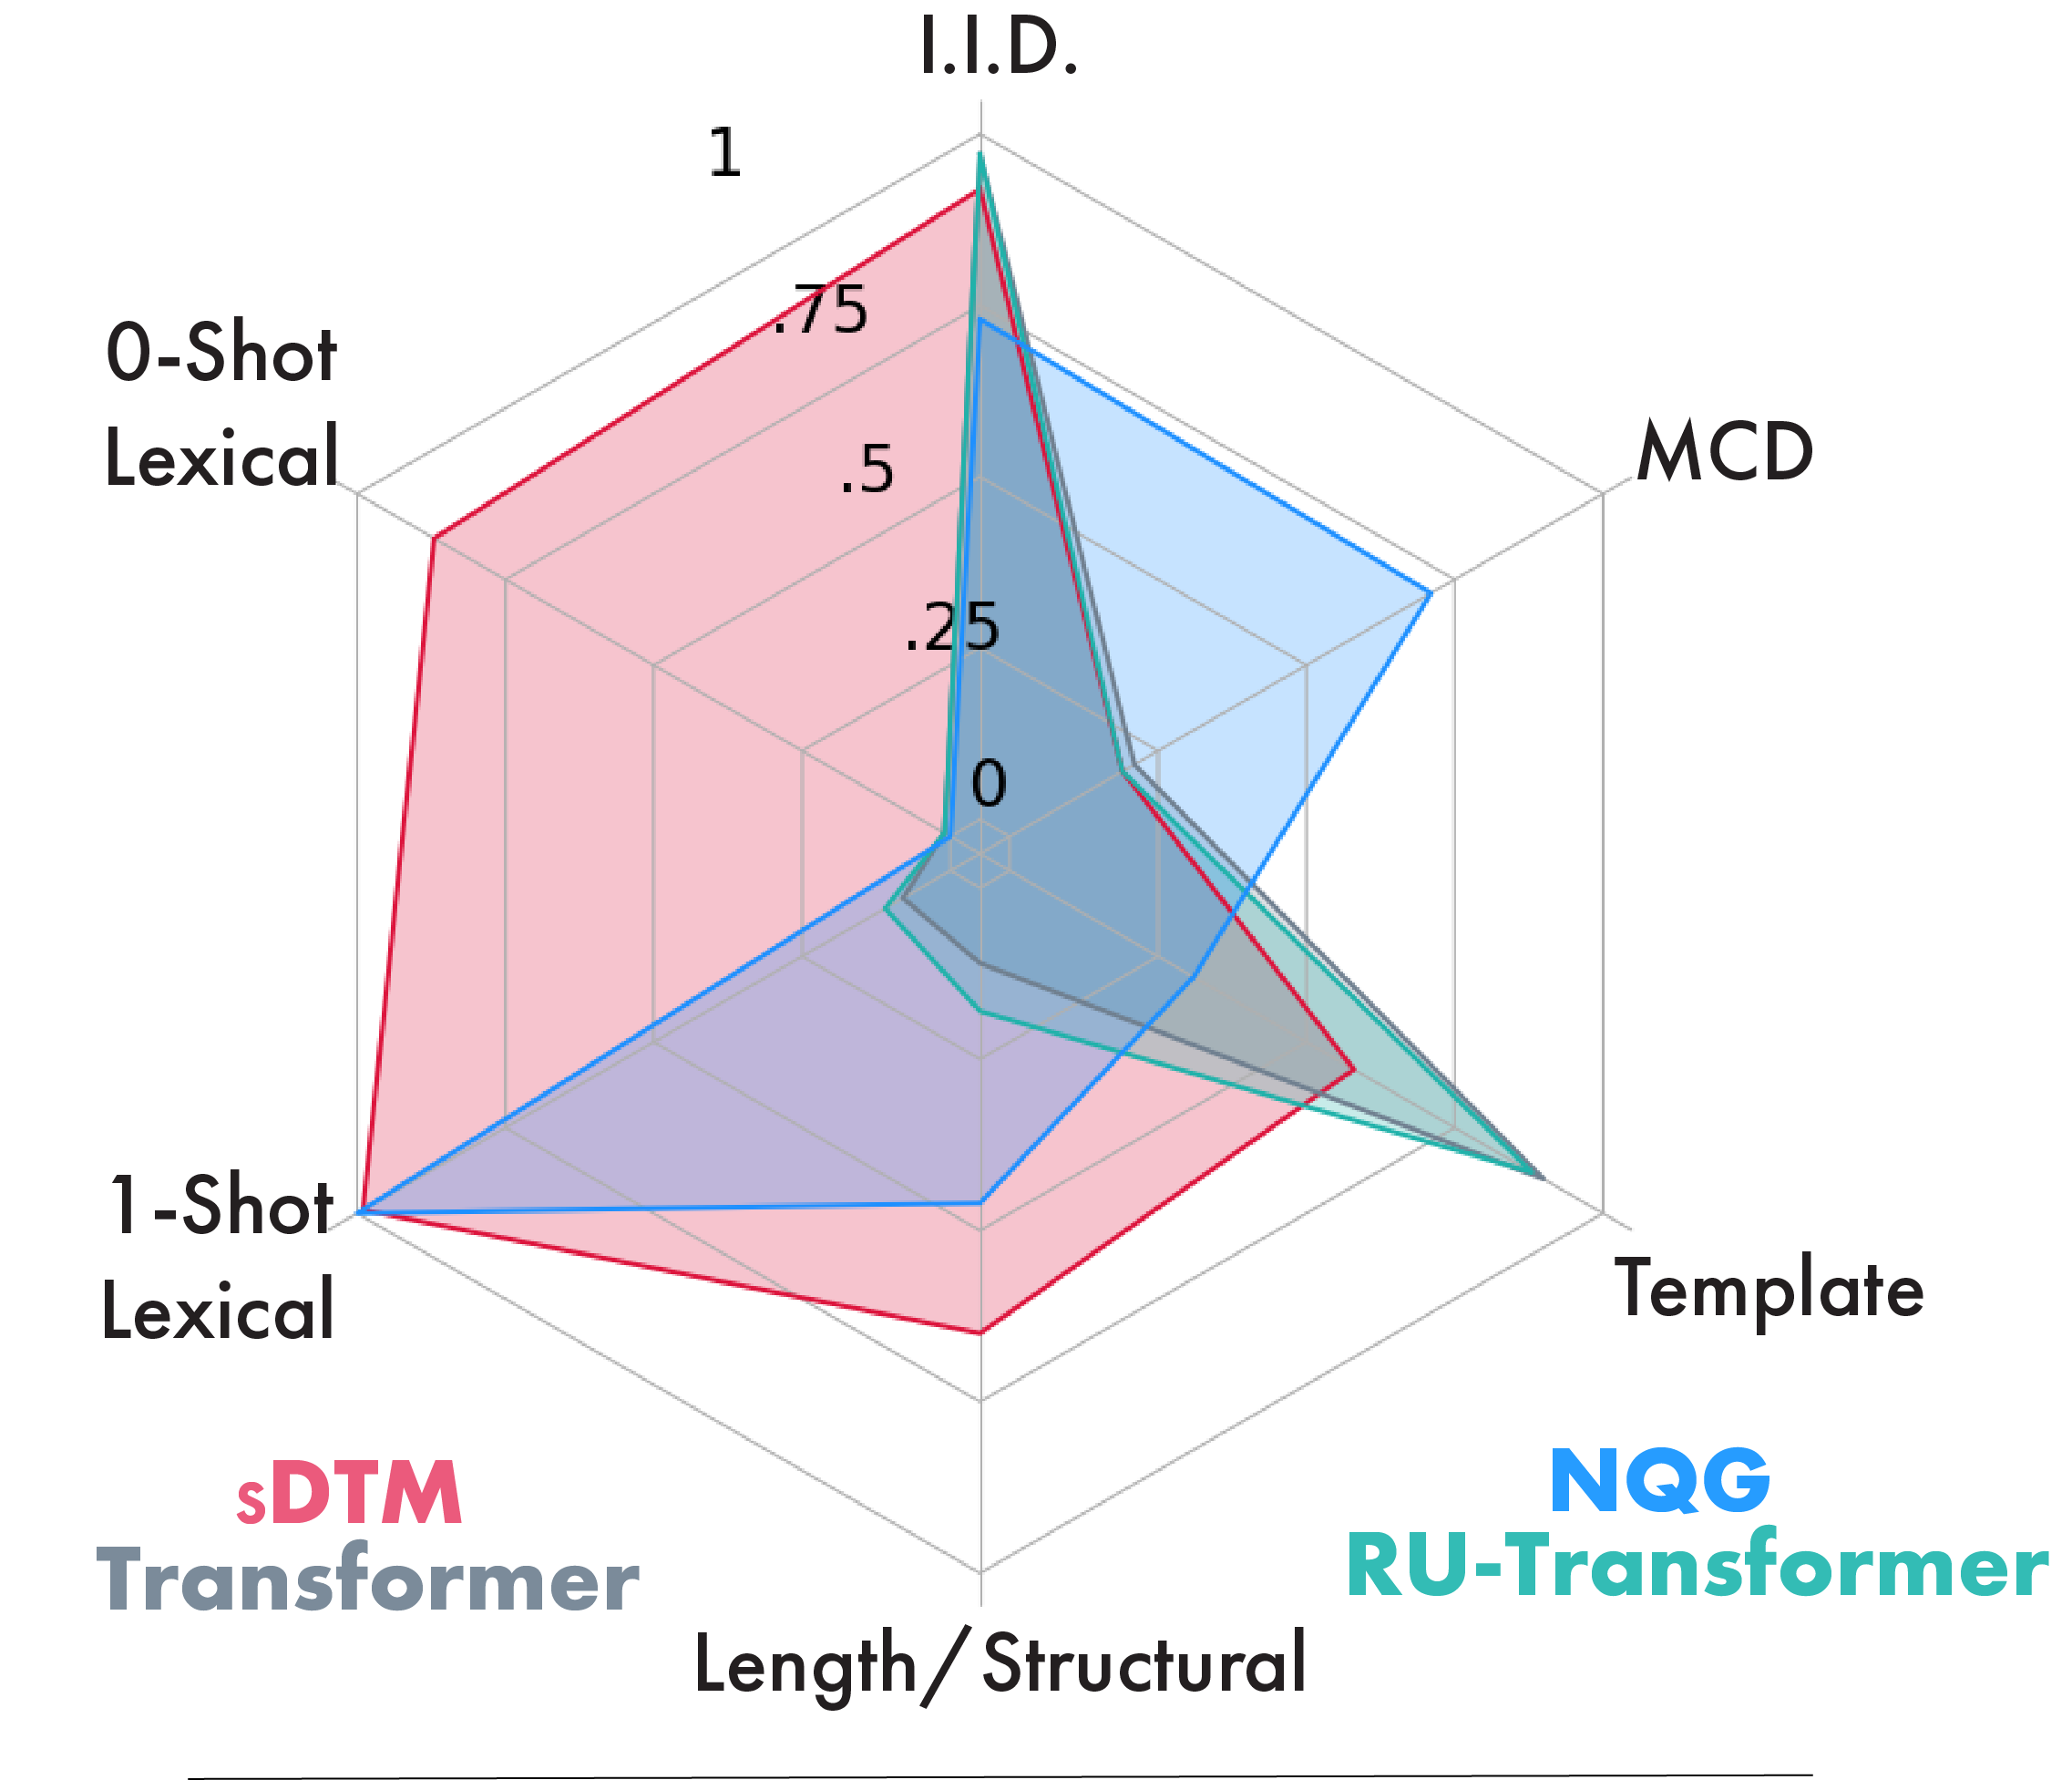
\includegraphics[width=\linewidth]{images/sdtm/tight_radar/radar_integrated_legend.png}
    %\vspace{-2.5em}
    \caption{Generalization ability of our approach (\sdtm) compared with baselines across various out-of-distribution shifts, averaged over different datasets. See \S \ref{sec:sdtm-results}.}
    \label{fig:enter-label}
    \vspace{-1.5em}
\end{wrapfigure}


Deep learning models achieve remarkable performance across a broad range of natural language tasks \citep{vaswani2017attention}, despite having difficulty generalizing outside of their training data, struggling with new words \citep{Lake_2018_GeneralizationSystematicityCompositional}, known words in new contexts \citep{keysers2020measuring}, and novel syntactic structures, like longer sequences with greater recursive depth \citep{kim-linzen-2020-cogs, li_slog_2023}. Increasingly this problem is addressed through data augmentation, which tries to make it less likely a model will encounter something unlike what it sees during training --- reducing the degree by which it has to generalize \citep{andreas_good-enough_2020, devlin_bert_2019,  guo_sequence-level_2020}. However, even models trained on vast quantities of data struggle when evaluated on examples unlike those seen during training \citep{kim2022uncontrolled}.


This stands in contrast to how humans process language, which enables robust generalization \citep{pinker2003language}. By breaking novel sentences into known parts, we can readily interpret phrases and constructions that we have never encountered before (e.g. `At the airport I smiled myself an upgrade', \citep{goldberg_constructions_2006}). Why do models trained on orders of magnitude more language data than a human hears in 200 lifetimes \citep{Griffiths2020UnderstandingHI} still fail to acquire some of language's most essential properties?

Central to language's generalizability is compositional structure \citep{partee1995lexical} where contentful units, like words, fit together in a structure, like a syntactic tree. Many classical approaches in NLP and Machine Learning attempt to induce a grammar from data in the hope of leveraging the same kinds of generalization seen in natural language \citep[e.g.][]{ klein2002generative, kim2019compound, steedman1987combinatory}. However, structured representations are not first-order primitives in most neural networks \citep{Marcus2001-MARTAM-10, Smolensky_1988}. Despite theoretical appeal, the strictures of purely discrete symbolic approaches have made them difficult to apply to the breadth of tasks and domains where deep learning models have proven successful \citep{furrer2020compositional}. In contrast, purely connectionist models --- like Transformers \citep{vaswani2017attention} --- struggle with the kinds of sample efficiency and robust generalization ubiquitous to human learning. 

Neurosymbolic methods attempt to integrate neural and symbolic techniques to arrive at a system that is both compositional and flexible \citep{nslr,garcez2008neural,GARNELO201917, Smolensky_1988}. While some neurosymbolic architectures achieve impressive compositional generalization, they are often brittle due to the symbolic core of their computation \citep{shaw-etal-2021-compositional}. These methods are hybrid neurosymbolic systems, where the primary computation is symbolic, and the neural network serves to parameterize the symbolic space. We take a different approach, one where symbolic operations happen in vector space. In our system, neural and symbolic computations are \textbf{unified} into a single space; we multiply and add vector-embedded symbolic structures instead of multiplying and adding individual neurons. %This technique is known as blending and superposition. % vector-embedded symbolic structures are blended together by superimposing them.

We introduce a new technique for representing trees in vector space called \fullrepname (\abvrepname). \abvrepname allows us to perform structural operations: transformations which change the structure of an object without changing the content. This is a crucial aspect of compositionality, where the structure and content can be transformed independently. We extend the Differentiable Tree Machine (\dtm), a system which operates over binary trees in vector space, into the Sparse Differentiable Tree Machine (\sdtm) to improve performance and applicability to a larger variety of tasks\footnote{Code available at \url{https://github.com/psoulos/sdtm}.}. While \dtm processes vector-embedded binary trees as the primitive unit of computation, the order of operations and argument selection is governed by a Transformer. We present results showing that this unified approach retains many of the desirable properties of more brittle symbolic models with regards to generalization, while remaining flexible enough to work across a far wider set of tasks. 
%Additionally we lay out a framework for evaluating generalization ability. Averaging scores across different tasks based on which of six different kinds of distributional shift they require a model to generalize to. 
While fully neural architectures or hybrid neurosymbolic techniques excel at certain types of generalization, we find that \dtm, with its unified approach,  excels across the widest array of shifts.

%In what follows we introduce a novel approach to unifying these lines of work;  a model architecture whose representational schema and internal operations are explicitly compositional, taking binary trees as its representational primitive. However, the order of operations applied and in what combination is governed by a transformer. We present results showing that this hybrid approach retains many of the desirable properties of more brittle symbolic models, while remaining flexible enough to work across a far wider set of tasks.

The main contributions from this paper are:
\begin{itemize}
  \item \fullrepname (\abvrepname), a method for representing binary trees in vector space as sparse tensors. (\S\ref{sec:sdtm-sparse-tpr})
  \item Bit-Shift Operating --- systematic and parallelized tree operations for \abvrepname. (\S\ref{sec:sdtm-diff-tree-ops})
  \item The introduction of Sparse Differentiable Tree Machine (\sdtm), architectural improvements to the \dtm to leverage \abvrepname and drastically reduce parameter and memory usage. (\S\ref{sec:sdtm-dtm-modifications})
  \item Techniques to apply \dtm to seq2seq tasks by converting sequences into trees. (\S\ref{sec:sdtm-seq2tree})
  \item Empirical comparisons between \sdtm and various baselines showing \sdtm's strong generalization across a wide variety of tasks. (\S\ref{sec:sdtm-results})
  %\item Ablation experiments to support our architectural decisions. (\paul{TODO on section})
\end{itemize}

\section{Related Work}
Work leveraging the generalizability of tree structures has a long history across Computer Science, Linguistics, and Cognitive Science \citep{chomsky_aspects_1965,mccarthy1960recursive, sakai1961syntax,  Smolensky1990TensorPV, steedman1987combinatory}. Much of classical NLP aims to extract structured representations from text like constituency or dependency parses \citep[for overview:][]{cuetos2013parsing, lopez2008statistical}. More recent work has shown the representations learned by sequence-to-sequence models without structural supervision can recover constituency, dependency, and part of speech information from latent representations in machine translation and language models \citep{belinkov2019analysis, blevins2018deep}. While those analyses show structural information is encoded, they stop short of showing that the representations themselves are tree-structured. Analyses inspired by Tensor Product Representations \citep{mccoy2018rnns, soulos2019discovering} and chart parsing \citep{murty2022characterizing} give an account of how representations become somewhat tree-structured over the course of training.% In particular correlating out-of-distribution performance with prevalence of structure.

Despite the apparent emergence of semi-structured representations in Transformers and LSTMs, these architectures still appear to struggle with the kinds of structural generalization that come easily to humans \citep{Lake_2018_GeneralizationSystematicityCompositional, kim_cogs_2020, keysers2020measuring}. A variety of approaches try to tackle this problem through meta-learning \citep{lake2019compositional, conklin2021meta}, data augmentation \citep{andreas_good-enough_2020}, or decomposing the task into separate parts \citep{ russin2019compositional, lindemann2023compositional}. The Relative-Universal Transformer \citep{csordas-etal-2021-devil} combines relative positional embeddings with a recurrent component, in an effort to emphasize local structures while allowing for unbounded computation.

%While in some cases effective these methods often have in-built costs in terms of training time, memory use, or domain generality - sometimes only working a small subset of tasks.



Explicitly tree structured network architectures have been introduced for RNNs \citep{socher-etal-2012-semantic}, LSTMs \citep{tai2015improved, dong2016language}, and Transformers \citep{wang2019tree, shiv2019novel}. However, these variants often do not outperform their unstructured counterpart on out-of-distribution challenges \citep{Soulos_2023_DifferentiableTreeOperations}. This may be because generalization requires both structured representations and operations that respect that structure. A separate line of work considers neural architectures that are used to parameterize components of a symbolic system \cite{kim2019compound, chen2020compositional} or fuzzy/probabilistic logic \citep{ijcai2020p243,BADREDDINE2022103649,Winters_Marra_Manhaeve_Raedt_2022, pmlr-v216-de-smet23a}. Similar to how vectors are embedded in trees in our work, some work  embeds vectors within logical systems \citep{rocktaschel-riedel-2016-learning, NEURIPS2023_bf215fa7}. Logic approaches to structure learning are also an active area of research \citep{Muggleton_1991_InductiveLogicProgramming, Shindo_Nishino_Yamamoto_2021}. Other approaches leverage explicit stack operations \citep{dusell2024stack, grefenstette2015learning, joulin2015inferring, yogatama2018memory}. NQG from \citet{shaw-etal-2021-compositional} combines the outputs from neural and symbolic models by inducing a grammar, but deferring to T5 \citep{t5} when that grammar fails. However the grammar's induction method has polynomial complexity with both dataset size and sequence length, which limits its application to larger tasks.

%Work that has neural components but a symbolic core: NQG (Compositional generalization and natural language variation: our model can handle both), Kim's NQCFG, The Nye work on program synthesis for SCAN, Neural symbolic stack machines.

%Meta-learning/auxiliary task and data augmentation (only works for lexical) approaches to compositionality.

%Work interpreting trees in neural networks (hewitt, murty, Tom's thesis, etc)

%Trees in neural networks (TreeRNN, TreeLSTM, Tree Transformer) can represent tree information, but don't have a way to modify trees with symbolic operations. TreeRNNs compress the tree, which makes it difficult to reconstruct the tree and perform systematic operations. For instance, we would want the encoding for a large tree passed through a left child operation to match the encoding of the left subchild built from the bottom up.

%Superposition Stacks function similar to our new sparse implicit method (cite joulin, gref, yogatama, dusell).

%Most similar to our work is that of \citet{Soulos_2023_DifferentiableTreeOperations}. In that work, trees are also represented in vector space and differentiable tree operations are derived.  However, they only apply their technique on Tree2Tree tasks, and their technique has limitations which make it computationally expensive. We show how to extend their approach to solve Seq2Tree and Seq2Seq tasks, and we also propose theoretical and applied changes to drastically improve the memory efficiency of their technique.

Vector Symbolic Architectures (VSAs) implement symbolic algorithms while leveraging high dimensional spaces \citep{plate, gayler2003vsa_jackendoff, kanerva2009hyperdimensional, kleyko2022}. VSAs are similar to uniform neurosymbolic approaches, although VSAs commonly lack a learning component. Our work extends that of \citet{Soulos_2023_DifferentiableTreeOperations} which can be viewed as integrating Deep Learning and VSAs. They introduce the Differentiable Tree Machine for Tree-to-Tree transduction. Here we instantiate a sparse Sequence-to-Sequence version with far fewer parameters and improved memory efficiency.

%The representation schema we use that enables this efficiency is similar to that of superposition stacks \cite{dusell2021learning}, though designed for tree-structures.

\begin{figure}
    \centering
    \includegraphics[width=\linewidth]{images/sdtm/sparse_coordinate_tree.pdf}
    \caption{An example representation using \fullrepname (\abvrepname). The values are N-dimensional vectors, and the tree positional indices are integer representations of positions in the tree. The absent child nodes of "The" (indices 4 and 6) are skipped with \abvrepname.}
    \label{fig:sparse-tpr}
\end{figure}

\section{Differentiable Tree Operations Over \fullrepname}
Representing trees in vector space enables us to perform differentiable structural operations on them. 
%However, before we can define the  operations, we need a representational format for embedding trees in vector space. 
\citet{Soulos_2023_DifferentiableTreeOperations} used Tensor Product Representations (TPRs) \citep{Smolensky1990TensorPV} for this purpose. TPRs use the tensor (or outer) product to represent trees in vector space (\S\ref{sec:sdtm-appendix-sparse-tprs}). Use of an outer product leads to a representation dimensionality that is multiplicative with both the embedding dimensionality and the number of possible tree nodes. Additionally, the number of nodes is itself an exponential function of the supported depth. This makes TPRs difficult to use in practice, given available memory is quickly exceeded as tree depth increases.

In this section, we introduce \fullrepname (\abvrepname), a new schema for representing trees in vector space. We then define a library of parallelized tree operations and how to perform these operations on \abvrepname.

\subsection{\fullrepname (\abvrepname)} 
\label{sec:sdtm-sparse-tpr}
Like TPRs, we want an encoding for trees that factorizes the representation into subspaces for \emph{structure} and \emph{content} respectively. This approach to representational spaces differs from models like an RNN and Transformer, which represent structure and content jointly in an unfactorized manner.
%many of today's popular neural networks which learn representations in an unfactorized manner. 
By separating the structure and content subspaces a priori, we can operate over these two spaces independently. This decision is motivated by the fact that distinct treatment of these spaces is an essential aspect of compositionality.

We derive our tree representation scheme from the sparse coordinate list (COO) format. COO stores tensor data in tuples of (indices [integers], values [any format], size [integers]). The indices are N-dimensional to simulate a tensor of arbitrary shape (e.g. including dimensions such as batch or length). When an index is not indicated in indices, it is assumed that the corresponding value is 0.

We give structural meaning to COO representations by defining one dimension of indices as the tree position occupied by a value vector. Our tree addressing scheme is based on Gorn addresses \citep{gorn+1967+77+115}: to get the tree position from an index, convert the index to binary and read from right to left. A left-branch is indicated by a $0$ and a right branch by a $1$. To distinguish between leading $0$s and left-branches (e.g. $010$ vs $10$), we start our addressing scheme at $1$ instead of $0$. This indicates that all $0$s to the left of the most-significant $1$ are unfilled and not left-branches. 
Figure \ref{fig:sparse-tpr} shows an example encoding of a tree with this approach. \abvrepname can be viewed as a TPR with certain constraints, and Section \ref{sec:sdtm-appendix-sparse-tprs} defines this equivalence and formally describes the memory savings.

Section \ref{sec:sdtm-previous-dtm-comparison} discusses the performance, memory, and parameter comparison between \dtm models which use standard TPRs and \abvrepname.

\subsection{Differentiable Tree Operations} \label{sec:sdtm-diff-tree-ops}

To operate on the trees defined in the previous section, we need a set of functions. We use a small library of only three: left-child (\leftcommand), right-child (\rightcommand), and \textbf{cons}truct (\cons) a new tree from a left and right subtree.\footnote{In LISP and expert systems literature, \leftcommand is referred to as \car, and \rightcommand is referred to as \cdr.} Although these three functions are simple, along with the control operations of conditional branching and equality-checking, these five functions are Turing complete \citep{mccarthy1960recursive}.

In addition to saving memory, \abvrepname also provides a more efficient method for performing differentiable tree operations. The operations defined in \citet{Soulos_2023_DifferentiableTreeOperations} require precomputing, storing, and applying linear transformations for \leftcommand, \rightcommand, and \cons. Since our values and tree positional indices are kept separate, we can compute the results of \leftcommand, \rightcommand, and \cons dramatically more efficiently using indexing, bit-shifts, and addition.

\begin{figure}
    \centering
    \includegraphics[width=\linewidth]{images/sdtm/left_and_right.pdf}
    \caption{Left: Performing \leftcommand (orange) and \rightcommand (blue). Right: visualizing the \leftcommand transformation which results in DP being placed at the root. Tree positional indices of $0$ and their corresponding values are discarded.}
    \label{fig:sparse-operations}
\end{figure}

Figure \ref{fig:sparse-operations} shows how we can perform \leftcommand directly on \abvrepname. \leftcommand is performed by indexing the even indices (i.e. those with a 0 in the least significant bit, which targets all of the nodes left of the root) and their corresponding values, then performing a right bit-shift on the indices. \rightcommand is symmetrical, except that we index for the odd positional indices and ignore position 1 in order to remove the previous root node. \cons is performed by left bit-shifting the positional indices from the left- and right-subtree arguments, then adding 1 to the newly shifted indices for the right argument. A new value $s$ can be provided for the root node.


Our network also needs to learn a \textit{program} over multiple operations differentiably. This involves the aforementioned structured operations, as well as differentiable selection of which operation to perform and on which trees. We take weighted sums over the three operations \leftcommand, \rightcommand, and \cons, as well as over potential trees. Specific details are discussed in the next section. The result of our weighted sum is coalesced, which removes duplicate positional indices by summing together all of the values that share a specific index. 
Formally, define the trees over which to perform \leftcommand \ $T_{L}$, \rightcommand \ $T_{R}$, and \cons \ $T_{CL}$ \& $T_{CR}$; $\vec{T}=[T_{L};T_{R};T_{CL};T_{CR}]$. We  also take a new value $s \in \mathbb{R}^{d}$ to be inserted ($\otimes$) at the new root node of the \cons operation, and a vector of operation weights $\vec{w} = (w_L,  w_R, w_C)$ which sum to 1.

\begin{equation} \label{eq:sdtm-output}
O(\vec{w}, \vec{T}, s) = w_L \leftcommand(T_{L}) + w_R \rightcommand(T_{R}) + w_C ( \cons(T_{CL}, T_{CR}) +  s \otimes r_{1})
\end{equation}

\section{The Sparse Differentiable Tree Machine (\sdtm)}
\label{sec:sdtm-dtm-modifications}

Our work extends the Differentiable Tree Machine (\dtm) introduced in \citet{Soulos_2023_DifferentiableTreeOperations} with the Sparse Differentiable Tree Machine (\sdtm). While similar to the original at a computational level, \sdtm represents a different implementation of these concepts that make it dramatically more parameter and memory efficient. We also introduce techniques to apply \sdtm to tasks with sequence input and output (seq2seq). 

\subsection{Overview} \label{sec:sdtm-dtm_sparse}
\begin{wrapfigure}{r}{0.45\linewidth}
    \centering
    \includegraphics[width=\linewidth]{images/sdtm/dtm-shrink.pdf}
    \caption{A schematic of how the three core components of the \dtm (agent, interpreter, and memory) relate to each other. Adapted from \citet{Soulos_2023_DifferentiableTreeOperations}.}
    \label{fig:dtm}
\end{wrapfigure}

\sdtm uses our \fullrepname schema across its components. Like the original \dtm, our model is comprised of an agent, interpreter, and memory (illustrated in Figure \ref{fig:dtm}). The Interpreter performs Equation \ref{eq:sdtm-output} by applying the bit-shifting tree operations from Section \ref{sec:sdtm-diff-tree-ops} and weighting the result. The output from the interpreter is written to the next available memory slot, and the last memory slot is taken as the output.

The Agent is a Transformer encoder that takes an encoding of the memory as input and produces the inputs for Equation \ref{eq:sdtm-output}: $\vec{w}$, $\vec{T}$, and $s$. Two special tokens, <OP> and <ROOT>, are fed into the Agent to represent $\vec{w}$ and $s$. Each time a tree is written to memory, a fixed-dimensional encoding of that tree is produced and fed as a new token to the agent (\S \ref{sec:sdtm-mha}). The agent soft-selects tree arguments for the interpreter, $\vec{T}$, by performing a weighted sum over the trees in memory. Figure \ref{fig:agent} in the Appendix contains a detailed diagram showing the flow of information for one layer of \sdtm.

The agent which implicitly parameterizes the conditional branching and control flow of the program is modeled by a Transformer, and it is possible for \sdtm to face some of the generalization pitfalls that plague Transformers. The design of \sdtm encourages compositional generalization through differentiable programs, but it does not strictly enforce the constraints of classical symbolic programs. As the results in Section \ref{sec:sdtm-results} show, \sdtm can learn generalizable solutions to some tasks despite the presence of a Transformer, but on some other tasks the issues with generalization are still present. 

\subsection{Pooling by attention} \label{sec:sdtm-mha}

Each tree in memory needs to have a fixed-dimensional encoding to feed into the agent regardless of how many nodes are filled. Commonly this is done via pooling, like taking the means of the elements in the tree, or a linear transformation in the case of the original \dtm. Instead, we use Pooling by Multi-headed Attention (PMA) \citep{pmlr-v97-lee19d}, which performs a weighted sum over the elements, where the weight is derived based on query-key attention.

Attention is permutation invariant to the ordering of key and value vectors, but it is important that our pooling considers tree position information. To enforce this, we convert the position indices to their binary vector representation $\vec{b}$. This leads to an asymmetrical vector with only positive values, so instead we represent left branches as $-1$ and keep right branches as $+1$. For example, position $5 \rightarrow [0,0,0,0,0,1,0,1] \rightarrow [0,0,0,0,0,1,-1,1]$. The input to our pooling function is the concatenation of this positional encoding $\vec{b}$ with the token embedding $\vec{x}$ at that position: $[\vec{x};\vec{b}]$. This method for integrating token and node position is similar to tree positional encoding from \citet{NEURIPS2019_6e091746}, except that we use concatenation and a linear transformation to mix the content and position information instead of addition.

Unlike standard self attention, we use a separate learnable parameter for our query vector $\vec{q} \in \mathbb{R}^{\text{num\_heads}\times\text{key\_dim}}$. We pass $[\vec{x};\vec{b}]$ through linear transformations to generate keys $\vec{k} \in \mathbb{R}^{\text{num\_heads}\times\text{key\_dim}}$ and values $\vec{v} \in \mathbb{R}^{\text{num\_heads}\times\text{value\_dim}}$. The result of this computation is always $z \in \mathbb{R}^{\text{num\_heads}\times\text{value\_dim}}$ given that $\vec{q}$ is fixed and does not depend on the input. The rest of the computation is identical to a Transformer with pre-layer normalization \citep{xiong2020layer}.

\subsection{Tree Pruning} \label{sec:sdtm-pruning}
While \fullrepname mean that trees with fewer filled nodes take up less memory, the way our model blends operations results in trees becoming dense.
%Our sparse tree representation works well when the trees themselves are sparse.
The interpreter returns a blend of all three operations at each step, including the \cons operation which increases the size of the representation by combining two trees. In practice even as the entropy of the blending distribution drops, the probability of any operation never becomes fully 0. This means that over many steps, trees start to become dense due to repeated use of \cons. In order to keep our trees sparse, we use pruning: only keeping the top-$k$ nodes as measured by magnitude. $k$ is a hyper-parameter that can be set along with the batch size depending on available memory. 

\subsection{Lexical Regularization} \label{sec:sdtm-lex-reg}
To aid lexical generalization, we add noise to our token embeddings. Before feeding an embedded batch into the model, we sample from a multi-variate standard normal for each position in each tree, adding the noise to the embeddings as a form of regularization \citep{bishop-noise}. Ablation results showing the importance of this regularization are available in Appendix \ref{sec:sdtm-lex-reg-ablation}. %Particularly on low-resource tasks, with a small input vocabulary --- like SCAN --- this regularisation proves essential. We believe this kind of regularisation forces the model to use a larger subspace to represent each token, which makes token representations more resilient to the kinds of novel contextualisations posed by lexical generalisation challenges. This approach to lexical regularisation can be easily applied to most models, and may improve generalisation in low-resource settings. 

%We find this regularization essential for lexical generalization as shown in \paul{TODO! Probably a table in the appendix}. We sample the noise from a standard normal distribution.

\subsection{Handling Sequential Inputs and Outputs}\label{sec:sdtm-seq2tree}
\paragraph{seq2tree} The original \dtm can only be applied to tasks where a tree structure is known for both inputs and outputs. Here we provide an extension to allow \dtm to process sequence inputs. To do this we treat each input token as a tree with only the root node occupied by the token embedding. We then initialize the tree memory with $N$ trees, one for each token in the input sequence. Figure \ref{fig:root-and-laud} left depicts the initial memory state for a sequence. The agent's attention mechanism is permutation-invariant, so in order to distinguish between two sequences which contain the same tokens but in different orders, we apply random sinusoidal positional encodings to the first $N$ tokens passed to the agent \citep{li2023representations, ruoss-etal-2023-randomized}. Random positional encodings sample a set of increasing integers from left-to-right instead of assigning a fixed position to each token. The purpose of \leftcommand and \rightcommand is to extract subtrees. Since in our seq2tree setting the input sequence is processed in a completely bottom-up manner, we restrict the agent and interpreter to only have a single operation: \cons. Use of a single operation to construct new trees from subtrees aligns the \dtm theoretically with the Minimalist Program \citep{10.7551/mitpress/9780262527347.001.0001}, which addresses natural language's compositionality in terms of a single operation: merge.
\paragraph{seq2seq} To handle sequence inputs and outputs we convert the output sequence to a tree. One method to convert the output sequence into a tree is to use a parser. Alternatively, when a parser is not available, we can embed a sequence as the \textbf{l}eft-\textbf{a}ligned leaves at \textbf{u}niform \textbf{d}epth (LAUD). Figure \ref{fig:root-and-laud} right shows how an output sequence can be embedded using LAUD. Since all of the non-terminal nodes are the same, we can hardcode the root argument to \cons. We insert a special token <EOB> to signify the end of a branch, similar to an <EOS> token.

\begin{figure}
    \centering
    \includegraphics[width=\linewidth]{images/sdtm/root_nodes_and_laud.pdf}
    \caption{Left: The memory state is initialized as a sequence of trees where only the root node contains a token. Right: An output sequence is embedded in a tree using the left-aligned uniform-depth (LAUD) scheme. <NT> and <EOB> are special tokens not in the original output sequence.}
    \label{fig:root-and-laud}
\end{figure}

\section{Results} \label{sec:sdtm-results}

\subsection{Baselines}
We consider models that are trained from scratch on the datasets they're evaluated on; while the compositional capabilities of large pre-trained models are under active debate \citep{kim2022uncontrolled}, we are interested in the compositional abilities of the underlying architecture --- rather than those that may result from a pre-training objective.
%believe that there is a benefit in developing models that learn from exposure to a single task. \paul{Other reasons to consider only models exposed to a task are for building human-like intelligence which isn't exposed to mass data as well as computing costs.} 
We compare \sdtm to two fully neural models, a standard Transformer \citep{vaswani2017attention} as well as a relative universal Transformer (RU-Transformer) which was previously shown to improve systematic generalization on a variety of tasks \citep{csordas-etal-2021-devil}. We also compare our model to a hybrid neurosymbolic system, NQG \citep{shaw-etal-2021-compositional, Sun_2023_ReplicationStudyCompositional}, a model which uses a neural network to learn a quasi-synchronous context-free grammar \citep{smith-eisner-2006-quasi}. NQG was introduced alongside NQG-T5, which is a modular system that uses NQG when the grammar produces an answer and falls back to a fine-tuned large language model T5 \citep{t5}. As mentioned at the beginning of this section, we only compare to NQG in this paper since we want to evaluate models that have not undergone significant pre-training.\footnote{NQG uses pre-trained BERT embeddings \citep{devlin_bert_2019}; it is unknown how much this pre-training helps the method.} Details related to data preprocessing (\S\ref{sec:sdtm-data-preprocessing}), model training (\S\ref{sec:sdtm-dtm-training}, \S\ref{sec:sdtm-baseline-training}), compute resources (\S\ref{sec:sdtm-compute-resources}), and dataset details (\S\ref{sec:sdtm-data-stats-samples}) are available in the Appendix. For all datasets, the reported results are the best exact match accuracies on the test set over five random seeds. Additional data on means and standard deviations across the five runs are shown in Section \ref{sec:sdtm-statistics}.

For each task, we test whether models generalize to samples drawn from various data distributions. Independent and identically distributed (\textbf{IID}) samples are drawn from a distribution shared with training data. We evaluate several out-of-distribution (OOD) shifts. \textbf{One-shot} lexical samples, while drawn from the same distribution as the training data, contain a word that was only seen in a single training sample. Similarly, \textbf{Zero-shot} lexical samples are those where the model is not exposed to a word at all during training. \textbf{Structural/length} generalization tests whether models can generalize to longer sequences (length) or nodes not encountered during training (structural). \textbf{Template} generalization withholds an abstract n-gram sequence during training, and then each test sample fits the template. Finally, maximum compound divergence (\textbf{MCD}) generates train and test sets with identical uni-gram distributions but maximally divergent n-grams frequencies \citep{keysers2020measuring}. Although models are often tested on a single type of generalization, we believe evaluating a model across a broad array of distributional shifts is essential for characterizing the robustness of its generalization performance.

\begin{table}
  \caption{\textbf{Active$\leftrightarrow$Logical accuracy.} Results are the best performance over five runs. The test sets are divided into IID, and OOD sets 0-shot lexical and structural. Parameter and memory usage is shown for the original \dtm with TPRs and our proposed sparse \dtm with and without pruning. Our modifications reduce the parameter count by almost two orders of magnitude. $^\ast$NQG was trained on a seq2seq version without parantheses because it was not able to learn the tree2tree training set.}
  \label{tab:activelogical}
  \centering
  \begin{tabular}{lllllll}
    \toprule
    Model & \multicolumn{3}{c}{Split}         \\
    \cmidrule(r){2-4}
    & IID & \begin{tabular}[c]{@{}l@{}}0-Shot \\ Lexical\end{tabular} & Structural \\
    \cmidrule(r){1-4}
    Transformer    & $1.0$ & $0.0$ & $0.0$ \\
    RU-Transformer & $1.0$ & $0.0$ & $.12$ \\
    NQG$^\ast$            & $.45$ & $0.0$ & $0.0$ \\
    \midrule
    & & & & Parameters & Memory (GB) & \begin{tabular}[c]{@{}l@{}}Relative \\ Speed\end{tabular} \\
    \midrule
    Original \dtm  & $1.0$ & $1.0$ & $1.0$ & 72M & 12.3 & 34  \\ 
    \sdtm  & $1.0$ & $1.0$ & $1.0$ & 1M & 9.7 & 2.5     \\
    \sdtm (pruned k=1024) & $1.0$ & $1.0$ & $.95$ & 1M & 1.8 & 1 \\
    \bottomrule
\end{tabular}
\end{table}

\subsection{Performance Regression (Active$\leftrightarrow$Logical)} \label{sec:sdtm-previous-dtm-comparison}
Active$\leftrightarrow$Logical is a tree2tree task containing input and output trees in active voice and logical forms \citep{Soulos_2023_DifferentiableTreeOperations}. Transforming a tree in active voice to its logical form simulates semantic parsing, and transforming a logical form tree to active voice simulates natural language generation. For this dataset, there are three test sets: IID, 0-shot lexical, and structural. In addition to the baselines listed in the previous section, we also compare our modified \sdtm to the original \dtm. This enables us to confirm that our proposed changes to decrease parameter count and memory usage while increasing inference speed does not lead to a performance regression. The results are show in Table \ref{tab:activelogical}.

The various \dtm models and Transformers all perform perfectly on the IID test set. NQG struggles to learn the Active$\leftrightarrow$Logical task, an example of the brittleness of hybrid neurosymbolic systems. Only the \dtm variants succeed on the OOD test sets. As anticipated, the RU-Transformer performs better than the standard Transformer with regards to structural generalization.

Comparing the original \dtm to \sdtm without pruning, we see a 70x reduction in parameter count from pooling by attention, a 20\% reduction in memory usage from fewer parameters and \abvrepname, as well as a roughly 13x speedup. We are able to gain even further memory savings and speed improvements due to the pruning method. The final two rows show that the pruning method has no impact on lexical generalization and a minor impact on structural generalization, while reducing memory usage by 5x and improving speed by 2.5x. The results from this experiment confirm that \sdtm is capable of matching \dtm performance on a previous baseline. However, since both \dtm and \sdtm perform near ceiling, it is difficult to isolate the effect of the proposed changes in this paper. We will investigate this question further in Section \ref{sec:sdtm-scan}. Next, we turn to tasks where the original \dtm could not be used.

\subsection{Scalability (FOR2LAM)}
FOR2LAM is a tree2tree program translation task to translate an abstract syntax tree (AST) in an imperative language (FOR) to an AST in a functional language (LAM) \citep{NEURIPS2018_d759175d}. Due to the depth of the trees in this dataset, \dtm is unable to fit a batch size of 1 into memory. This makes FOR2LAM a good dataset to test the scalability of \sdtm to more complex samples. We augment the FOR2LAM dataset with a 0-shot lexical test set. During training, only two variable names appear: `x' and `y'. For the 0-shot test, we replace all occurrences of x in the test set with a new token `z'. We are unable to test \dtm on FOR2LAM because a batch size of 1 does not fit into memory due to the depth of the trees in the dataset.


Results on FOR2LAM are shown on the left side of Table \ref{tab:for2lam_geoquery}. NQG suffers with scale (see \ref{sec:sdtm-baseline-training}), and we were unable to include results for it on FOR2LAM due to training and evaluation exceeding 7 days. All other models do well on the in-distribution test set, but only \dtm is able to achieve substantive accuracy on the 0-shot lexical test. \dtm's performance is impressive given work on data augmentation has shown the difficulty of few-shot generalization is inversely proportional to vocabulary size \citep{patel2022revisiting}, with smaller vocabulary tasks being more challenging. This 0-shot challenge is from 2 variables (x, y) to 3 (x, y, z), making it difficult enough that both transformer variants score 3\%.

\subsection{Seq2Tree (GeoQuery)}

\begin{table}
\caption{\textbf{Accuracies on FOR2LAM and GeoQuery.} Results are the best performance over five runs. NQG cannot be evaluated on FOR2LAM because it takes over a week to train. $^\dag$Results taken from \citet{shaw-etal-2021-compositional}. $^\ast$We report the results from a replication study of NQG where the result on the Length split differed substantially from the original result \citep{Sun_2023_ReplicationStudyCompositional}.}
\centering
\begin{tabular}{lcccccc}
\toprule
& \multicolumn{2}{c}{\textbf{FOR2LAM}} & \multicolumn{4}{c}{\textbf{GeoQuery}} \\
\cmidrule(r){2-3} \cmidrule(l){4-7}
Model & IID & 0-shot lexical & IID & Length & Template & TMCD \\
\midrule
Transformer & 1.0 & .03 & .88 & .26 & .79 & .40 \\
RU-Transformer & 1.0 & .03 & .87 & .25 & .77 & .37 \\
NQG$^\dag$ & -- & -- & .76 & .37/.26$^\ast$ & .62 & .41 \\
\midrule
\sdtm & 1.0 & .61 & .73 & .20 & .20 & .36 \\
\bottomrule
\end{tabular}
\label{tab:for2lam_geoquery}
\end{table}

GeoQuery is a natural language to SQL dataset \citep{zelle1996learning} where a model needs to map a question stated in natural language to a correctly formatted SQL query, including parentheses to mark functions and arguments. We use the parentheses and function argument relationship as the tree structure for our output. In this format, GeoQuery is a seq2tree task, and we follow the description from Section \ref{sec:sdtm-seq2tree}.  We use the same preprocessing and data as \citet{shaw-etal-2021-compositional}. The TMCD split for GeoQuery \citep{shaw-etal-2021-compositional} extends MCD to natural language datasets instead of synthetic languages. GeoQuery is a very small dataset, with a training set containing between 440 and 600 samples, depending on the split. Like FOR2LAM, we are unable to test \dtm on GeoQuery because a batch size of 1 does not fit into memory due to the depth of the trees in the dataset.


Results for GeoQuery are shown on the right side of Table \ref{tab:for2lam_geoquery}. This is the most difficult task that we test because of the small training set, and the natural language input is not draw from a synthetic grammar. Given this, a potential symbolic solution to this task might be quite complex. We find that both NQG and \dtm perform worse than the two Transformer variants on the IID test set. This also holds true for the Template split, where Transformers outperform the neurosymbolic models. On the Length and TMCD splits, all of the baselines achieve roughly the same performance while \dtm performs slightly worse --- the degree of variation in the input space and small training set appear to make it difficult for \sdtm to find a compositional solution. 

It is worth noting that there is substantial room for improvement across every model on GeoQuery. The small dataset with high variation poses a problem for both compositional methods of \sdtm and NQG. It is possible that with sufficient data, GeoQuery's latent compositional structure could be identified by NQG and DTM, but the released GeoQuery dataset has only on the order of 500 training examples. Given all methods struggle to model the IID split, we refrain from drawing substantive conclusions based on minor differences in accuracy on this single task in isolation from the rest of the results. 

%\paul{Can we justify this performance a bit?}

\subsection{Seq2Seq (SCAN)} \label{sec:sdtm-scan}
SCAN is a synthetic seq2seq task with training and test variations to examine out-of-distribution generalization \citep{Lake_2018_GeneralizationSystematicityCompositional}. To process seq2seq samples, we follow the description in Section \ref{sec:sdtm-seq2tree}. We compare two methods for embedding the output sequence into a tree by writing a parser for SCAN's output and comparing this to the left-aligned uniform-depth trees (LAUD). In addition to the standard test splits from SCAN, we introduce a 0-shot lexical test set as well.

\begin{table}
  \caption{\textbf{SCAN accuracy.} Results are the best performance over five runs. MCD scores are calculated as the average of the three MCD splits. $^\dag$Results from \citet{shaw-etal-2021-compositional}. $^\ast$Results from \citet{Sun_2023_ReplicationStudyCompositional}.}
  \label{tab:scan}
  \centering
  \begin{tabular}{lllllll}
    \toprule
    Model & \multicolumn{6}{c}{Split}         \\
    \cmidrule(r){2-7}
    & IID & 1-shot lexical & 0-shot lexical & Length & Template & MCD \\
    \midrule
    Transformer & 1.0 & .08 & 0.0 & .07 & 1.0 & .02 \\
    RU-Transformer & 1.0 & .11 & 0.0 & .19 & 1.0 & .01 \\
    NQG$^\dag$ & 1.0$^\ast$ & 1.0 & 0.0 & 1.0 & 0.0$^\ast$ & 1.0     \\
    \midrule
    \sdtm (parse trees)     & 1.0   & .99 & .99 & .75 & .95 & .03  \\
    \sdtm (LAUD trees) & 1.0 & .87 & .98 & .06 & .98 & 0.0 \\
    \dtm (parse trees) & 0.0 & 0.0 & 0.0 & 0.0 & 0.0 & 0.0 \\
    \bottomrule
\end{tabular}
\end{table}

Since the trees in SCAN are not very deep, we are able to compare \sdtm to \dtm to isolate the effect of pooling by attention (\S\ref{sec:sdtm-mha}). We modify the original \dtm to handle sequential inputs and outputs as described in Section \ref{sec:sdtm-seq2tree}. Replacing the linear transformation in \dtm with pooling by attention in \sdtm leads to drastically better results; \dtm is unable to perform well even on the simple IID split, whereas \sdtm performs well across many of the splits.

All baselines perform well on the IID test set, showing that they have learned the training distribution well. Transformer variants perform poorly on lexical, length, and MCD splits. 
%The RU-Transformer does better than the standard Transformer on the length split, but \citet{csordas-etal-2021-devil} showed that the RU-Transformer needs an easier length shift to increase its performance more.
The Transformers and \sdtm perform well on the Template split while NQG completely fails. Along with the results from GeoQuery, which showed weak \sdtm performance on the Template split and strong performance from both Transformers, it seems that the Transformer architecture is robust under template shifts between training and testing. \sdtm is the only model to perform well on the 0-shot lexical test set, whereas NQG is the only model able to perform well on the MCD test set. The two \sdtm rows compare models trained with output trees from a parser or LAUD encoding. The main performance difference is on the Length split, where the structurally relevant information in the parse trees is necessary for \sdtm to perform well. It is not necessary to have structured input for the model to perform well on length generalization as long as the output is structured.

\section{Conclusions} \label{sec:sdtm-conclusion}
We introduced the Sparse Differentiable Tree Machine (\sdtm) and a novel schema for efficiently representing trees in vector space: \fullrepname (\abvrepname).
Unlike the fully neural and hybrid neurosymbolic baselines presented here, \sdtm takes a unified approach whereby symbolic operations occur in vector space. While not perfect --- \sdtm struggles with MCD and Template shifts, as well as the extremely small GeoQuery dataset --- the model generalizes robustly across the \textit{widest variety} of distributional shifts. \sdtm is also uniquely capable of zero-shot lexical generalization, likely enabled by its factorization of content and structure.

While these capacities for generalization are shared with the original \dtm, our instantiation is computationally efficient (representing a 75x reduction in parameters) and can be applied to seq2seq, seq2tree, and tree2tree tasks. Our work reaffirms the ability of neurosymbolic approaches to bridge the flexibility of connectionist models with the generalization of symbolic systems. We believe continued focus on efficient neurosymbolic implementations can lead to architectures with the kinds of robust generalization, scalability, and flexibility characteristic of human intelligence.
\definecolor{pink}{rgb}{0.8549019607843137, 0.5450980392156862, 0.7647058823529411}

\chapter{Recurrent Transformers Trade-off Parallelism for Length Generalization on Regular Languages} \label{chap:chap-4}


\begin{singlespace}         % you can also use `onehalfspace` to relax the spacing
    This chapter is reprinted from \fullcite{soulos2024recurrent}. Licensed under CC BY 4.0.
\end{singlespace} 

%% remove the following and add your chapter text here
\section{Abstract}
    Transformers have achieved remarkable success in Natural Language Processing but struggle with state tracking and algorithmic reasoning tasks, such as modeling Regular Languages. In contrast, Recurrent Neural Networks (RNNs) exhibit perfect generalization modeling Regular Languages. To bridge this gap, we explore Recurrent Transformer variants that incorporate chunking, balancing the parallelizability of Transformers with the sequential processing of RNNs. We identify layer-recurrence as the key type of recurrence that allows Recurrent Transformers to succeed in modeling Regular Languages. Further analysis indicates a rapid decline in generalization performance as chunk size increases beyond two, though with an exponential decrease in training time. This study underscores the critical role of layer-recurrence and chunk size in Recurrent Transformers, highlighting the trade-off between generalization capabilities and parallelism. Code available at \url{https://github.com/IBM/recurrent-chunked-models-regular-languages}.%While small chunk sizes improve the ability of Recurrent Transformers to model Regular Languages and, by extension, more complex language structures, the decrease in training speed makes it costly to train models with small chunk sizes on large datasets. Our results suggest that optimizing chunk size, enhancing the speed of Recurrent Transformers, or adding recurrence during fine-tuning are important steps for improving training Recurrent Transformers at scale. 
    
    \section{Introduction}
    
    \begin{figure}[t]
        \centering
        \includegraphics[width=.5\linewidth]{images/recurrent/generalization_performance_talk.pdf}
        \caption{The generalization performance of Transformers with various types of recurrence. Lengths to the left of the dashed line are in-distribution, and lengths to the right are out-of-distribution.}
        \label{fig:results-summary}
    \end{figure}
    
    Despite the remarkable success of Transformers \citep{vaswani2017attention} in Natural Language Processing (NLP), the architecture continues to struggle with state tracking and algorithmic reasoning \citep{hahn_theoretical_2020, bhattamishra_ability_2020, deletang_neural_2022}. The Chomsky Hierarchy \citep{chomsky_three_1956, chomsky_certain_1959} provides a framework for classifying tasks based on difficulty, and \citet{deletang_neural_2022} demonstrated that Transformers show profound weaknesses across the hierarchy.
    
    Regular Languages, the simplest class in the Chomsky Hierarchy, are an important benchmark for evaluating the reasoning capabilities of neural network architectures. Regular Languages can be represented using a Finite State Machine with no access to an external memory \citep{hopcroft_introduction_2006}. If an architecture fails to learn Regular Languages in a robust and generalizable way, it is unlikely that it will succeed on more challenging problems further up the hierarchy. On three out of four Regular Language tasks from \citet{deletang_neural_2022}, Transformers fail to generalize to longer samples than those encountered in the training set (see the \textcolor{pink}{pink} line in Figure \ref{fig:results-summary}). Such experimental studies are supported by theoretical results that highlight the Transformer's inability to model regular languages over arbitrary input lengths \citep{merrill_parallelism_2023, strobl_what_2024}.
    
    Understanding the necessary modifications to Transformers to improve their performance modeling Regular Languages is an important step in ascending the hierarchy towards mildly-context sensitive languages, which are hypothesized to encapsulate human language \citep{joshi_tree_1985, joshi_convergence_1990}. Furthermore, the modifications might shed light on important inductive biases for human-like language processing leading to improved generalization, reasoning, and sample efficiency.
    
    The performance of Transformers contrasts with the results from various Recurrent Neural Network (RNN) architectures, such as Simple Recurrent Networks \citep{elman_finding_1990} and Long Short-Term Memory networks \citep{hochreiter_long_1997}, both of which exhibit perfect length generalization on the same four Regular Language tasks. RNNs can track intermediate states by updating the recurrent vector that is passed forward to future tokens. For a sequence of $T$ tokens, an RNN will perform $T$ computation steps, allowing it to maintain and update a state representation at each step. In contrast, standard Transformers are non-recurrent, and a Transformer with $L$ layers will process $T$ tokens in $L$ computation steps, regardless of the sequence length. \citet{liu_transformers_2022} demonstrated that Transformers with at least $L=\text{log}(T)$ layers can learn shortcut solutions for modeling automata. While these shortcut solutions perform well in-distribution, they are brittle and fail to generalize to longer samples, revealing a limitation in the Transformers' ability to model Regular Languages effectively.
    
    The lack of a recurrent mechanism allows Transformers to process an entire sequence in parallel using masking and teacher forcing. However, the absence of recurrence makes generalization challenging for Transformers on certain algorithmic tasks where maintaining intermediate states would be beneficial \citep{merrill_parallelism_2023}. In a separate line of work, researchers have investigated combining Transformers with recurrent mechanisms to improve the performance in modeling long sequences \citep{hutchins_block-recurrent_2022, ding_ernie-doc_2021, bulatov_recurrent_2022} and tasks where Transformers fail \citep{ju_staircase_2022}. In this paper, we address how Recurrent Transformers affect generalization.
    
    \begin{figure}
        \centering    \includegraphics[width=.7\linewidth]{images/recurrent/architectures.pdf}
        \caption{Computation graphs for an RNN, Transformer, and Recurrent Transformer over four tokens. The boxes with the same number can be calculated in parallel, and the number indicates the sequential step of computation (for example, box 3 cannot be calculated until boxes 1 and 2 are finished). Boxes within the same chunk are highlighted in light orange and share the same number. Recurrent connections are red, and attention connections are green. The Recurrent Transformer depicted has a chunk size of 2.}
        \label{fig:architectures}
    \end{figure}
    
    Recurrent Transformer variants introduce the notion of \textit{chunking} to interpolate between the fast, parallelizable architecture of a standard Transformer and the slower, sequential architecture of RNNs. Within a chunk, all tokens are processed in parallel, while a recurrent connection is established between chunks. At the extremes, a chunk size of 1 processes inputs similarly to an RNN, whereas a chunk size equal to the maximum sequence length is equivalent to a standard Transformer. Figure \ref{fig:architectures} illustrates the computation graph and associated parallelizability for an RNN, a Transformer, and a Recurrent Transformer. It is important to note that the slowdown from adding recurrent processing to Transformers only occurs when teacher forcing is enabled, typically during training. When a standard Transformer generates tokens in an autoregressive setting, it must proceed token-by-token and has no parallelism benefits over a Recurrent Transformer.
    
    
    We start by defining Token Layer Recurrence, the type of recurrence implemented by RNNs. We show that Staircase Attention \citep{ju_staircase_2022} satisfies Token Layer Recurrence at a chunk size of 1, whereas Block-Recurrent Transformer (BRT) \citep{hutchins_block-recurrent_2022} does not. We validate this finding empirically by showing that Staircase Attention generalizes well on the Regular Language tasks and BRT fails (Figure \ref{fig:results-summary}). We also define Chunk Layer Recurrence, a less restrictive version of Token Layer Recurrence, and investigate the relationship between larger chunk sizes and generalization performance. While large chunk sizes are faster and more amenable to large-scale training, we find that small chunk sizes consistently perform better for every architecture in terms of length generalization. Although models with smaller chunk sizes generalize better, we observe that these smaller chunk sizes lead to training speeds an order of magnitude slower than a standard Transformer. This work highlights the importance of either increasing the speed of Recurrent Transformers, finding the optimal chunk size for a specific task, or adding recurrence during post-training.
    
    The primary contributions of this paper are:
    \begin{itemize}
    \item Defining Token Layer Recurrence and Chunk Layer Recurrence.
    \item Evaluating three chunk-based models, namely Staircase Attention, Block-Recurrent Transformer, and RegularGPT, on Regular Language tasks.
    \item Identifying Staircase Attention as a Recurrent Transformer that generalizes well on the tasks and satisfies Chunk Layer Recurrence.
    \item Investigating the relationship between chunk size and generalization performance.
    \item Demonstrating the impact of chunk size on training speed and therefore scalability.
    \end{itemize}
    
    \section{Related Work}
    
    \paragraph{The Chomsky Hierarchy}
    The Chomsky Hierarchy \citep{chomsky_three_1956, chomsky_certain_1959} identifies Formal Language computations by increasing complexity based on the required grammar to model the computation. Each level of the hierarchy can be modeled by a finite state machine with access to increasingly expressive data structures. One line of research is to map Neural Network architectures to levels of the hierarchy \citep{bhattamishra_ability_2020, deletang_neural_2022, strobl_what_2024}. \citet{borenstein_what_2024} extend previous work on Regular Language recognition to Regular Language modeling by using KL Divergence between model predictions and probabilistic finite-state automata.
    
    \paragraph{Transformers and their limitations}
    Standard Transformers are known to possess computational limitations due to the attention mechanism \citep{merrill_parallelism_2023, strobl_what_2024}. \citet{liu_transformers_2022} showed theoretically and empirically that Transformers are able to learn shortcuts to simulate an automata with $T$ tokens in $\text{log}(T)$ layers. The learned shortcuts are brittle and do not generalize well. \citet{chi_transformer_2023} modify a Transformer to succeed on Regular Language tasks, although their architecture has degraded performance on natural language modeling. 
    
    \paragraph{Recurrent Neural Networks}
    Recurrent Neural Networks (RNNs) were developed to process sequential information, with a particular focus on language processing \citep{jordan_serial_1997, elman_finding_1990}. Two significant improvements to RNNs were the introduction of gating \citep{hochreiter_long_1997, cho-etal-2014-learning} and attention \citep{bahdanau_neural_2015}. Researchers have investigated the computability of RNNs from a formal language perspective \citep{siegelmann_computational_1995, chen_recurrent_2018, nowak_representational_2023, svete_recurrent_2023}.
    
    \paragraph{Recurrent Transformers}
    Prior work has investigated adding recurrent mechanisms into Transformers. \citet{ju_staircase_2022} introduce Staircase Attention and show improvements on entity-tracking and language modeling.  \citet{hutchins_block-recurrent_2022} and \citet{didolkar_temporal_2022} contemporaneously published Transformer architectures which use cross attention to a set of recurrent vectors to improve modeling long range sequences. \citet{bulatov_recurrent_2022} showed improvements on long range modeling by adding recurrent memory tokens to Transformers. \citet{chowdhury_investigating_2024} investigated the relationship between Transformer depth-wise recurrence and chunk-wise recurrence on various tasks.
    
    \paragraph{Transformer Length Generalization}
    Since Transformers lack recurrence, positional embeddings are used to signify the order of tokens. Different types of positional embeddings can improve length generalization \citep{csordas-etal-2021-devil, ruoss-etal-2023-randomized, shaw_self-attention_2018, su_roformer_2024, zhou_transformers_2024, kazemnejad_impact_2023, press_train_2021}, although \citet{deletang_neural_2022} and \citet{ruoss-etal-2023-randomized} showed that none of the positional embeddings that they tested allowed Transformers to generalize well on Regular Languages.
    
    \section{Architectures}
    \begin{figure}[ht]
        \centering
        \includegraphics[width=.2\linewidth]{images/recurrent/attention patterns.pdf}
        \caption{Attention patterns for standard attention and Staircase Attention.}
        \label{fig:attention-patterns}
    \end{figure}
    
    We briefly describe three architectures that we test. For additional details, please see the original papers. For each architectures, task, and chunk size, we run a hyperparameter search to find the best setting for that combination. We then train five randomly initialized models with the best setting and report these results. Training details for each architecture can be found in Appendix \ref{sec:recurrent-training-details}.
    
    The three architectures we discuss below use the notion of dividing an input sequence $X=\{X_0,\dots X_{T-1}\}$ of length $T$ into chunks $K=\{K_0,\dots K_{\lceil T/C\rceil}\}$ of size $C$ where $K_i=\{{X_{i\times C},\dots X_{(i+1)\times C - 1}}\}$. Each architecture processes chunks in different ways.
    
    \paragraph{Token Layer Recurrence} RNNs implement recurrence through the property that the output for a token $X_{i,l}$ at sequence position $i$ and layer $l$ depends on the output of a previous token at layer $l$: $X_{i,l}=f(X_{<i,l},\dots)\ \forall i>0$. Meanwhile, the state of token $X_{i,l}$ in a Transformer with causal attention depends only on states at $l-1$: $X_{i,l}=f(\{X_{<i,l-1}\})$. Token layer recurrence allows a network to iteratively update a state as new information is processed. For a treatment of token layer recurrence and generalization in Linear RNNs, see \citet{fan_advancing_2024} and \citet{merrill_illusion_2024}.
    
    \paragraph{Chunk Layer Recurrence} When the chunk size is greater than 1, the property of layer recurrence is violated. Consider a chunk size of $C=2$. $X_0$ and $X_1$ will be processed in parallel, which means that $X_{1,l}=f(X_{0,l-1},X_{1,l-1})$. Thus, we define Chunk Layer Recurrence similarly to Token Layer Recurrence but with chunks: $K_{i,l}=f(K_{<i,l},\dots)\ \forall i>0$. A model that satisfies Chunk Layer Recurrence will satisfy Token Layer Recurrence when the chunk size is set to 1.
    
    \subsection{Staircase Attention}
    Staircase Attention \citep{ju_staircase_2022} staggers the chunks so that each consecutive chunk attends to the previous chunk after one level of processing. The differences between standard attention and Staircase Attention are depicted in Figure \ref{fig:attention-patterns}. By staggering the chunks, Staircase Attention satisfies Chunk Layer Recurrence. In order to speed up the model, Staircase Attention uses a Universal Transformer \citep{dehghani_universal_2018} so that multiple chunks at different layers can be processed in parallel. \citet{ju_staircase_2022} show that Staircase Attention succeeds on two state tracking tasks where Transformers fail, but they did not consider how the model generalizes out-of-distribution. Here, we look at state tracking tasks and how well the model generalizes to longer sequences. Staircase Attention also shows competitive performance on language modeling tasks. The authors consider chunk sizes 8, 16, and 32 for the algorithmic tasks, and chunk sizes 32, 64, and 128 for the language modeling tasks. Their results generally show improved performance with smaller chunk sizes, at the cost of a slower model.
    
    
    \subsection{Block-Recurrent Transformers}
    Block-Recurrent Transformers (BRT) \citep{hutchins_block-recurrent_2022} integrate the recurrent connection as cross attention between the current chunk and a set of recurrent tokens. This allows the output of the chunk to use information from previous chunks. The recurrent tokens are updated by using cross-attention to the chunk tokens, and the recurrent tokens are passed along to the next chunk. Crucially, the recurrent tokens attend to the input of the chunk instead of the output. This means that BRT \textit{does not} satisfy Chunk Layer Recurrence. Inspired by gating in LSTMs \citep{hochreiter_long_1997}, BRT experiments with different gate configurations for the recurrent tokens. This design is similar to the Temporal Latent Bottleneck \citep{didolkar_temporal_2022} which was published concurrently. BRT shows improved performance on long sequence language modeling as measured by perplexity. They uses a chunk size of 512, two orders of magnitude larger than the chunks we consider in this paper.
    
    \subsection{RegularGPT}
    RegularGPT \citep{chi_transformer_2023} is not a recurrent model, but we include it in our experiments since it uses chunked processing. Rather than enforcing a sequential processing of chunks, RegularGPT leverages attention masking to enforce a divide-and-conquer strategy. RegularGPT does not support chunk size 1. The divide-and-conquer strategy is implemented using a Universal Transformer with sliding dilated attention masks and dynamic depth. RegularGPT has good length generalization on the Regular Language tasks from \citep{deletang_neural_2022} using a chunk size of $C=2$. However, while RegularGPT improves performance on the Regular Language tasks, it leads to worse performance in Language Modeling as measured by perplexity on length extrapolation when compared to other models designed for long contexts. RegularGPT shows decreased performance going from chunk size 2 to 3. Here, we investigate whether this trend continues for larger chunk sizes 4 and 8. On language modeling, RegularGPT is tested with chunk sizes 32, 64, 128, and 256. The authors find that chunk size 128 works the best but underperforms baselines.
    
    \begin{figure}[t]
        \centering
        \includegraphics[width=.5\linewidth]{images/recurrent/chunk_1_poster.pdf}
        \caption{Average generalization performance of token recurrent architectures (chunk size 1) on Regular Language tasks. Bars indicate minimum and maximum values across five random seeds.}
        \label{fig:fully-recurrent}
    \end{figure}
    
    \section{Results}
    \subsection{Datasets}
    We test the three models on the four Regular Language tasks from \citet{deletang_neural_2022}: Even Pairs, Parity Check, Cycle Navigation, and Modular Arithmetic (Simple). For more details about these tasks, see Appendix \ref{sec:recurrent-dataset-details}. We follow the same procedure as \citet{deletang_neural_2022} and train our models on sequences up to length 40, and during test time we evaluate our model on sequences up to length 500. The score is the average accuracy measured over sequences from length 1 to 500.
    
    \subsection{Token Recurrent Transformers (Chunk Size 1)}
    We first test Recurrent Transformers with a chunk size of 1 to see if a token recurrent model can replicate the performance of a simple RNN. The results are shown in Figure \ref{fig:fully-recurrent}. Both the RNN and Staircase Attention achieve perfect generalization across the four tasks. BRT performs better than the Transformer in Parity Check and Even Pairs but does not provide any benefit in Cycle Navigation or Modular Arithmetic. These results validate that adding the right type of recurrence to Transformers can improve generalization, but a chunk size of 1 forgoes the parallelism benefits of Transformers.
    
    \begin{figure}
        \centering
        \includegraphics[width=\linewidth]{images/recurrent/results_all_notebook.pdf}
        \caption{Average generalization performance by chunk size across five random seeds. The shaded regions represent minimum and maximum values. The dashed gray bar represents chance performance. The dashed pink line represents the average Transformer performance, and the dotted pink link represents the max Transformer performance. Transformer results are drawn from \citet{deletang_neural_2022}.}
        \label{fig:results}
    \end{figure}
    
    \subsection{Performance degrades with larger chunk sizes}
    In order to see how much we can scale up Recurrent Transformers, we test how the generalization performance changes as we increase parallelism through larger chunk sizes. Figure \ref{fig:results} shows the performance of each architecture and chunk size combination on the four tasks. Across all of the tasks and architectures, generalization drops as chunk sizes increases, except for Even Pairs where all models succeed.
    
    \paragraph{Even Pairs} Even Pairs is the only Regular Language task where a standard Transformer is capable of generalizing well, although with high variance as seen by the difference between max and average Transformer results indicated by the pink lines. All three models achieve consistent generalization on Even Pairs regardless of the chunk size. 
    
    \paragraph{Parity Check} Transformers struggle on Parity Check with the best performing Transformer barely performing above chance. Both Recurrent models are capable of perfect generalization at chunk size 1, and all three chunked models succeed at chunk size 2, although BRT shows high variance. At chunk size 4, BRT fails to generalize, RegularGPT succeeds across every seed, and Staircase Attention generally performs well. 
    
    \paragraph{Cycle Navigation} After Even Pairs, Cycle Navigation is the second easiest Regular Language task, with the best Transformer achieving a score of 0.6. For chunk sizes 1 and 2, Staircase Attention generalizes well, but by chunk size 4 the performance drops drastically. RegularGPT does well at chunk size 2, and is capable of succeeding at chunk size 4, although with high variance. By chunk size 8, RegularGPT no longer generalizes. BRT fails to generalize at any chunk size.
    
    \paragraph{Modular Arithmetic} Transformers struggle on Modular Arithmetic, and the best performing model barely does better than chance. BRT fails to generalize and shows similar results as the Transformer. RegularGPT does well at chunk size 2, but it's performance decreases linearly down to chance by chunk size 8. Staircase Attention does well across all of the chunk sizes tested.
    
    The main takeaway as evidenced by Figure \ref{fig:results} is that smaller chunk sizes work better. Staircase Attention with chunk size 2 consistently performs well. We do not find much difference between chunk size 1 and 2 in terms of generalization performance for Staircase Attention, and as we will show in the next section, chunk size 2 is roughly twice as fast as chunk size 1.
    
    
    \subsection{Training Speed} \label{sec:recurrent-training-speed}
    The previous section showed that smaller chunk sizes for Recurrent Transformers work better. However, smaller chunk sizes also lead to a slower step time when the architectures are trained in a non-autoregressive setting with teacher forcing. In this section, we quantify how much slower Recurrent Transformers are at different chunk sizes.
    
    Figure \ref{fig:speed} shows the relative step time slowdown of Staircase Attention for different chunk sizes and sequence lengths. We use relative speed in order to profile the model speed since relative speed transfers across hardware and implementation details. In order to calculate the relative speed, we divide the forward and backward step time for Staircase Attention by the step time for a parallel Transformer.  When a chunk size is greater than or equal to the sequence length, the performance should mirror that of a standard Transformer since the sequence will be processed without recurrence, which we see for chunk size 4096. The figure shows that doubling the chunk size roughly makes the model twice as fast. As the sequence length increases so does the slowdown, until a certain point, after which the slowdown decreases. Staircase Attention does not compute the full $O(N^2)$ attention, so at larger lengths the slowdown compared baseline starts to recede. The relative step slowdown for BRT is shown in Appendix \ref{sec:recurrent-brt-performance}.
    
    
    \begin{figure}
        \centering
        \includegraphics[width=\linewidth]{images/recurrent/Staircase_notebook.pdf}
        \caption{Staircase Attention relative step time slowdown compared to a baseline Transformer, represented by the dashed line. Relative slowdown is the ratio of model step time by baseline step time.}
        \label{fig:speed}
    \end{figure}
    
    Importantly, at test time when performing autoregressive generation, Recurrent Transformers do not incur a speed penalty for their recurrence. This means that these architectures are a fixed training cost, and they yield the same cost when generating text in an autoregressive manner.
    
    \subsection{Navigating the generalization-parallelism frontier}
    The previous two sections illustrate the challenge of scaling Recurrent Transformers. On one hand, large chunk sizes lead to faster training, whereas on the other hand, smaller chunk sizes are more consistent across different tasks. Ideally, we would have a theoretical basis for identifying optimal chunk size in a natural language corpus. Even on the four simple tasks explored here, Staircase Attention has a different optimal chunk size for each task. While chunk size 2 generalizes well on every task, Modular Arithmetic is amenable to chunk size 8 which is roughly 3 times faster than than chunk size 2.
    
    \section{Conclusion and Future Work}
    
    We investigated the performance of Recurrent Transformers on Regular Language tasks. While Transformers generalize poorly on these tasks, we found that Staircase Attention with a small chunk size generalizes well. 
    
    The small chunk size required for consistent generalization poses some roadblocks for scaling up Staircase Attention. Two immediate questions are whether we can define the optimal chunk size that supports generalization for a given task, and whether we can instill recurrence during post-training instead of pre-training.
    
    In order to scale up Recurrent Transformers for reasoning, we want to find the largest chunk size for a dataset that retains good generalization. For instance, Python is whitespace sensitive, so one trivial chunking hypothesis is to break chunks on newlines. A similar idea is to break natural language on punctuation, conjunctions, and relative clauses. Future work should investigate the properties that define optimal chunks.
    
    One way to alleviate the slowdown from recurrent training is to start with a pre-trained LLM and instill recurrence during post-training. Recurrent processing is more likely to be helpful on datasets where reasoning is important. For example, recurrence would be much more beneficial on datasets with explicit intermediate reasoning \citep{nye_show_2021, wei_chain_2022} than a dataset with a list of independent facts. Some forms of post-training are inherently autoregressive like reinforcement learning from human feedback \citep{christiano_deep_2017}, process supervision \citep{lightman_lets_2024}, and preference optimization \citep{pang_iterative_2024}; in these cases there will be no extra cost of using Recurrent Transformers over standard Transformers. Future work should investigate how recurrent post-training can be performed on a model pre-trained in a parallel manner.
    
    An additional direction to consider is how Recurrent Transformers perform within the scaling laws \citep{kaplan_scaling_2020, hoffmann_training_2022}. If recurrence is a useful inductive bias, models may converge faster with better generalization while being trained on shorter sequences. This might make Recurrent Transformers more competitive when evaluated on computational budget as opposed to only looking at the time for a training step.
    
    This work showed that some Recurrent Transformers can successfully model Regular Languages. Human language is hypothesized to be Mildly Context-Sensitive \citep{joshi_tree_1985, joshi_convergence_1990}, and we can climb the Chomsky Hierarchy \citep{chomsky_three_1956, chomsky_certain_1959} by integrating Recurrent Transformers with differentiable stacks \citep{joulin_inferring_2015, grefenstette2015learning} to model Context-Free Language and differentiable trees \citep{pmlr-v202-soulos23a} to model Mildly Context-Sensitive Languages. Recent work by \citet{dusell2024stack} showed that Transformers with Stack Attention improve modeling of Context-Free transformations, but their models do not perform well out-of-distribution. Integrating Staircase Attention into their model may help Transformers perform better on Context-Free transformations in and out-of distribution.
    
\chapter{Something about Stack Transformers} \label{chap:chap-5}


%% remove the following and add your chapter text here
\section{Introduction}


%% add more main text technical chapters if you have

%%%%%%%%%%%%%%%%%%%%%%%%%%% END MAIN MATTER %%%%%%%%%%%%%%%%%%%%%%%%%%%%



%%%%%%%%%%%%%%%%%%%%%%%%%%%%% BACK MATTER %%%%%%%%%%%%%%%%%%%%%%%%%%%%%%

%%%% BIBLIOGRAPHIC REFERENCES
\BibTextSpacing                         % text spacing for each bib item
\fancyhead[L]{\nouppercase \leftmark}
\printbibliography[title={Bibliographic references},
    heading=bibintoc, notcategory=mypapers]
\clearpage                              % flushes out floating header


%%%% Appendix chapter (same header format as the main chapters)
%% if you do not have appendix chapters, then comment them out
\MainTextSpacing                    
\fancyhead[L]{\appendixname\ \thechapter. \nouppercase \leftmark}


%%%% necessary customization for the appendix and headers
\appendix 
\makeatletter
\addtocontents{toc}{\protect\renewcommand\protect\cftchappresnum{\@chapapp\ }}
\makeatother
\renewcommand{\thechapter}{\Alph{chapter}}

\chapter{Appendix for Discovering the Compositional Structure of Vector Representations with Role Learning Networks} \label{chap:appendix-a}

%% add your chapter text here
\section{Designed role schemes} \label{sec:rldn-role-schemes}
We use six hand-specified role schemes as a baseline to compare the learned role schemes against. Examples of each role scheme are shown in Table \ref{tab:rolestwo}.

\begin{enumerate}
	\item Left-to-right (LTR): Each filler's role is its index in the sequence, counting from left to right.
	\item Right-to-left (RTL): Each filler's role is its index in the sequence, counting from right to left.
	\item Bidirectional (Bi): Each filler's role is a pair of indices, where the first index counts from left to right, and the second index counts from right to left.
	\item Tree: Each filler's role is given by its position in a tree. This depends on a tree parsing algorithm.
	\item Wickelroles (Wickel): Each filler's role is a 2-tuple containing the filler before it and the filler after it. \citep{wickelgren1969context}
	\item Bag-of-words (BOW): Each filler is assigned the same role. The position and context of the filler is ignored.
\end{enumerate}

\begin{table*}[ht]
    \centering
     \resizebox{\textwidth}{!}{
    \begin{tabular} {l|llll|llllll}
    \toprule
    & 3 & 1 & 1& 6 & 5 & 2 & 3 & 1 & 9 & 7 \\ \midrule
    Left-to-right & 0 &1&2&3 & 0&1&2&3&4&5\\
Right-to-left & 3&2&1&0 & 5&4&3&2&1&0 \\
Bidirectional & (0, 3)&(1, 2)&(2, 1)&(3, 0) & (0, 5)&(1, 4)&(2, 3)&(3, 2)&(4, 1)&(5, 0) \\
Wickelroles & \#\_1& 3\_1& 1\_6& 1\_\# & \#\_2& 5\_3& 2\_1& 3\_9& 1\_7& 9\_\# \\
Tree & L& RLL& RLR& RR & LL& LRLL& LRLR& LRRL& LRRR& R \\
Bag of words & r$_0$&r$_0$&r$_0$&r$_0$ & r$_0$&r$_0$&r$_0$&r$_0$&r$_0$&r$_0$ \\ \bottomrule
\end{tabular}
}
    \caption{\label{tab:rolestwo}The assigned roles for two sequences, 3116 and 523197. Table reproduced from \citet{mccoy2018rnns}.}
\end{table*}

\section{ROLE regularization} \label{sec:rldn-role-regulatization}

Letting $\mA = \{\va_t \}_{t=1}^T$, the regularization term applied during ROLE training is $R = \lambda (R_1 + R_2 + R_3)$, where $\lambda$ is a regularization hyperparameter and:
\begin{align*} %\label{eq:reg}
    R_1(\mA) &= \sum_{t=1}^T\sum_{\rho=1}^{n_\rR} [\va_t]_\rho(1-[\va_t]_\rho); \hspace{1.5mm}\\
    R_2(\mA) &= -\sum_{t=1}^{T}\sum_{\rho=1}^{n_\rR} [\va_t]_\rho^2; \hspace{1.5mm}\\
    R_3(\mA) &= \sum_{\rho=1}^{n_\rR} \left( [\vs_\mA]_\rho (1 - [\vs_\mA]_\rho) \right)^2
\end{align*}
Since each $\va_t$ results from a softmax, its elements are positive and sum to 1. Thus the factors in $R_1(\mA)$ are all non-negative, so $R_1$ assumes its minimal value of 0 when each $\va_t$ has binary elements; since these elements must sum to 1, such an $\va_t$ must be one-hot.
$R_2(\mA)$ is also minimized when each $\va_t$ is one-hot because when a vector's $L^1$ norm is 1, its $L^2$ norm is maximized when it is one-hot. Although each of these terms individually favor one-hot vectors, empirically we find that using both terms helps the training process.
In a discrete symbolic structure, each position can hold at most one symbol, and the final term $R_3$ in \RLN's regularizer $R$ is designed to encourage this.
In the vector $\vs_\mA = \sum_{t=1}^T \va_t$, the $\rho^\r{th}$ element is the total attention weight, over all symbols in the string, assigned to the $\rho^{\r{th}}$ role: in the discrete case, this must be 0 (if no symbol is assigned this role) or 1 (if a single symbol is assigned this role).
Thus $R_3$ is minimized when all elements of $\vs$ are 0 or 1 ($R_3$ is similar to $R_1$, but with squared terms since we are no longer assured each element is at most 1). It is important to normalize each role embedding in the role matrix \textbf{R} so that small attention weights have correspondingly small impacts on the weighted-sum role embedding.

\section{RNN trained on SCAN} \label{sec:rldn-rnn-scan}

To train the standard RNN on SCAN, we ran a limited hyperparameter search similar to the procedure in \citet{Lake_2018_GeneralizationSystematicityCompositional}. Since our goal was to produce a single embedding that captured the entire input sequence, we fixed the architecture as a GRU with a single hidden layer. We did not train models with attention, to investigate whether a standard RNN could capture compositionality in its single bottleneck encoding. The remaining hyperparameters were hidden dimension and dropout. We ran a search over the hidden dimension sizes of 50, 100, 200, and 400 as well as dropout with a value of 0, .1, and .5 applied to the word embeddings and recurrent layer. Each network was trained with the Adam optimizer \citep{kingma2015adam} and a learning rate of .001 for 100,000 steps with a batch-size of 1. The best performing network had a hidden dimension or 100 and dropout of .1.

\section{\RLN\ trained on SCAN} \label{sec:rldn-role-scan}

For the \RLN\ models trained to approximate the GRU encoder trained on SCAN, we used a filler dimension of 100, and a role dimension of 50 with 50 roles available. For training, we used the Adam \citep{kingma2015adam} optimizer with a learning rate of .001, batch size 32, and an early stopping patience of 10. The role assignment module used a bidirectional 2-layer LSTM \citep{hochreiter_long_1997}. We performed a hyperparameter search over the regularization coefficient $\lambda$ using the values in the set [.1, .02, .01]. The best performing value was .02, and we used this model in our analysis.

%A co-occurrence matrix of filler:role bindings is shown in Figure \ref{fig:scan-heatmap}.

The algorithm below characterizes our post-hoc interpretation of which roles the Role Learner will assign to elements of the input to the SCAN model. This algorithm was created by hand based on an analysis of the Role Learner's outputs for the elements of the SCAN training set. The algorithm works equally well on examples in the training set and the test set; on both datasets, it exactly matches the roles chosen by the Role Learner for 98.7\% of sequences (20,642 out of 20,910).%\footnote{This figure of 98.7\% is so constant across datasets presumably because the synthetic nature of the SCAN dataset means that any reasonably-sized sample from it will be similarly representative of the entire dataset.}

\section{A role-assignment algorithm implicitly learned by the SCAN seq2seq encoder} \label{sec:rldn-Alg}

The input sequences have three basic types that are relevant to determining the role assignment: sequences that contain \textit{and} (e.g., \textit{jump around left and walk thrice}), sequences that contain  \textit{after} (e.g., \textit{jump around left after walk thrice}), and sequences without \textit{and} or \textit{after} (e.g., \textit{turn opposite right thrice}). Within commands containing \textit{and} or \textit{after}, it is convenient to break the command down into the command before the connecting word and the command after it; for example, in the command \textit{jump around left after walk thrice}, these two components would be \textit{jump around left} and \textit{walk thrice}. 

\begin{itemize}
    \item Sequence with \textit{and}:
    \begin{itemize}
        \item Elements of the command before \textit{and}:
        \begin{itemize}
            \item Last word: 28
            \item First word (if not also last word): 46
            \item \textit{opposite} if the command ends with \textit{thrice}: 22
            \item Direction word between \textit{opposite} and \textit{thrice}: 2
            \item \textit{opposite} if the command does not end with \textit{thrice}: 2
            \item Direction word after \textit{opposite} but not before \textit{thrice}: 4
            \item \textit{around}: 22
            \item Direction word after \textit{around}: 2
            \item Direction word between an action word and \textit{twice} or \textit{thrice}: 2
        \end{itemize}
        \item Elements of the command before \textit{and}:
        \begin{itemize}
            \item First word: 11
            \item Last word (if not also the first word): 36
            \item Second-to-last word (if not also the first word): 3
            \item Second of four words: 24
        \end{itemize}
        \item \textit{and}: 30
    \end{itemize}
    \item Sequence with \textit{after}:
    \begin{itemize}
        \item Elements of the command before \textit{after}:
        \begin{itemize}
            \item Last word: 8
            \item Second-to-last word: 36
            \item First word (if not the last or second-to-last word): 11
            \item Second word (if not the last or second-to-last word): 3
        \end{itemize}
        \item Elements of the command after \textit{after}:
        \begin{itemize}
            \item Last word: 46
            \item Second-to-last word: 4
            \item First word if the command ends with \textit{around right}: 4
            \item First word if the command ends with \textit{thrice} and contains a rotation: 10
            \item First word if the command does not end with \textit{around right} and does not contain both \textit{thrice} and a rotation: 17
            \item Second word if the command ends with \textit{thrice}: 17
            \item Second word if the command does not end with \textit{thrice}: 10
        \end{itemize}
        \item \textit{after}: 17 if no other word has role 17 or if the command after \textit{after} ends with \textit{around left}; 43 otherwise
    \end{itemize}
    \item Sequence without \textit{and} or \textit{after}:
    \begin{itemize}
        \item Action word directly before a cardinality: 4
        \item Action word before, but not directly before, a cardinality: 34
        \item \textit{thrice} directly after an action word: 2
        \item \textit{twice} directly after an action word: 2
        \item \textit{opposite} in a sequence ending with \textit{twice}: 8
        \item \textit{opposite} in a sequence ending with \textit{thrice}: 34
        \item \textit{around} in a sequence ending with a cardinality:  22
        \item Direction word directly before a cardinality: 2
        \item Action word in a sequence without a cardinality: 46
        \item \textit{opposite} in a sequence without a cardinality: 2
        \item Direction after \textit{opposite} in a sequence without a cardinality: 26
        \item \textit{around} in a sequence without a cardinality: 3
        \item Direction after \textit{around} in a sequence without a cardinality: 22
        \item Direction directly after an action in a sequence without a cardinality: 22
    \end{itemize}
\end{itemize}

\noindent
To show how this works with an example, consider the input \textit{jump around left after walk thrice}. The command before \textit{after} is \textit{jump around left}. \textit{left}, as the last word, is given role 8. \textit{around}, as the second-to-last word, gets role 36. \textit{jump}, as a first word that is not also the last or second-to-last word gets role 11. The command after \textit{after} is \textit{walk thrice}. \textit{thrice}, as the last word, gets role 46. \textit{walk}, as the second-to-last word, gets role 4. Finally, \textit{after} gets role 17 because no other elements have been assigned role 17 yet. These predicted outputs match those given by the Role Learner.

\section{Discussion of the algorithm} \label{sec:rldn-AlgDisc}

We offer several observations about this algorithm.

\begin{enumerate}
    \item 
This algorithm may seem convoluted, but a few observations can illuminate how the roles assigned by such an algorithm support success on the SCAN task. First, a sequence will contain role 30 if and only if it contains \textit{and}, and it will contain role 17 if and only if it contains \textit{after}. Thus, by implicitly checking for the presence of these two roles (regardless of the fillers bound to them), the decoder can tell whether the output involves one or two basic commands, where the presence of \textit{and} or \textit{after} leads to two basic commands and the absence of both leads to one basic command. Moreover, if there are two basic commands, whether it is role 17 or role 30 that is present can tell the decoder whether the input order of these commands also corresponds to their output order (when it is \textit{and} in play, i.e., role 30), or if the input order is reversed (when it is \textit{after} in play, i.e., role 17).

With these basic structural facts established, the decoder can begin to decode the specific commands. For example, if the input is a sequence with \textit{after}, it can begin with the command after \textit{after}, which it can decode by checking which fillers are bound to the relevant roles for that type of command.

It may seem odd that so many of the roles are based on position (e.g., ``first word" and ``second-to-last word"), rather than more functionally-relevant categories such as ``direction word." However, this approach may actually be more efficient: Each command consists of a single mandatory element (namely, an action word such as \textit{walk} or \textit{jump}) followed by several optional modifiers (namely, rotation words, direction words, and cardinalities). Because most of the word categories are optional, it might be inefficient to check for the presence of, e.g., a cardinality, since many sequences will not have one. By contrast, every sequence will have a last word, and checking the identity of the last word provides much functionally-relevant information: if that word is not a cardinality, then the decoder knows that there is no cardinality present in the command (because if there were, it would be the last word); and if it is a cardinality, then that is important to know, because the presence of \textit{twice} or \textit{thrice} can dramatically affect the shape of the output sequence. In this light, it is unsurprising that the SCAN encoder has implicitly learned several different roles that essentially mean the last element of a particular subcommand.
\item
The algorithm does not constitute a simple, transparent role scheme. But its job is to describe the representations that the original network produces, and we have no a priori expectation about how complex that process may be. The role-assignment algorithm implicitly learned by ROLE is interpretable locally (each line is readily expressible in simple English), but not intuitively transparent globally. We see this as a positive result, in two respects.

First, it shows why ROLE is crucial: no human-generated role scheme would provide a good approximation to this algorithm. Such an algorithm can only be identified because ROLE is able to use gradient descent to find role schemes far more complex than any we would hypothesize intuitively. This enables us to analyze networks far more complex than we could analyze previously, being necessarily limited to hand-designed role schemes based on human intuitions about how to perform the task. 

Second, when future work illuminates the computation in the original SCAN GRU seq2seq decoder, the baroqueness of the role-assignment algorithm that ROLE has shown to be implicit in the seq2seq encoder can potentially explain certain limitations in the original model, which is known to suffer from severe failures of systematic generalization outside the training distribution (Lake and Baroni, 2018). It is reasonable to hypothesize that systematic generalization requires that the encoder learn an implicit role scheme that is relatively simple and highly compositional. Future proposals for improving the systematic generalization of models on SCAN can be examined using ROLE to test the hypothesis that greater systematicity requires greater compositional simplicity in the role scheme implicitly learned by the encoder.

\item
While the role-assignment algorithm of A.8.1 may not be simple, from a certain perspective, 
it is quite surprising that it is not far more complex. Although ROLE is provided 50 roles to learn to deploy as it likes, it only chooses to use 16 of them (only 16 are ever selected as the $\argmax(\va_t)$; see Sec. 6.1). Furthermore, the SCAN grammar generates 20,910 input sequences, containing a total of 151,688 words (an average of 7.25 words per input). This means that, if one were to generate a series of conditional statements to determine which role is assigned to each word in every context, this could in theory require up to 151,688 conditionals (e.g., ``if the filler is `jump’ in the context `walk thrice after \underline{\hspace{.25 in}} opposite left’, then assign role 17''). However, our algorithm involves just 47 conditionals. This reduction helps explain how the model performs so well on the test set: If it used many more of the 151,688 possible conditional rules, it would completely overfit the training examples in a way that would be unlikely to generalize. The 47-conditional algorithm we found is more likely to generalize by abstracting over many details of the context.

\item
Were it not for ROLE’s ability to characterize the representations generated by the original encoder in terms of implicit roles, providing an equally complete and accurate interpretation of those representations would necessarily require identifying the conditions determining the activation level of each of the 100 neurons hosting those representations. It seems to us grossly overly optimistic to estimate that each neuron’s activation level in the representation of a given input could be characterized by a property of the input statable in, say, two lines of roughly 20 words/symbols; yet even then, the algorithm would require 200 lines, whereas the algorithm in A.8.1 requires 47 lines of that scale. Thus, by even such a crude estimate of the degree of complexity expected for an algorithm describing the representations in terms of neuron activities, the algorithm we find, stated over roles, is 4 times simpler.


\end{enumerate}

\section{TPEs trained on sentence embedding models} \label{sec:rldn-tpe-sentences}

For each sentence embedding model, we trained three randomly initialized TPEs for each role scheme and selected the best performing one as measured by the lowest MSE. For each TPE, we used the original filler embedding from the sentence embedding model. This filler dimensionality is 25 for SST, 300 for SPINN and InferSent, and 620 for Skipthought. We applied a linear transformation to the pre-trained filler embedding where the input size is the dimensionality of the pre-trained embedding and the output size is also the dimensionality of the pre-trained embedding. This linearly transformed embedding is used as the filler vector in the filler-role binding in the TPE. For each TPE, we use a role dimension of 50. Training was done with a batch size of 32 using the Adam optimizer with a learning rate of .001.

To generate tree roles from the English sentences, we used the constituency parser released in version 3.9.1 of Stanford CoreNLP \citep{klein2003accurate}.

\section{\RLN\ trained on sentence embedding models} \label{sec:rldn-role-sentences}

For each sentence embedding model, we trained three randomly initialized \RLN\ models and selected the best performing one as measured by the lowest MSE. We used the original filler embedding from the sentence embedding model (25 for SST, 300 for SPINN and InferSent, and 620 for Skipthought). We applied a linear transformation to the pre-trained filler embedding where the input size is the dimensionality of the pre-trained embedding and the output size is also the dimensionality of the pre-trained embedding. This linearly transformed embedding is used as the filler vector in the filler-role binding in the TPE. We also applied a similar linear transformation to the pre-trained filler embedding before input to the role learner LSTM. For each \RLN\ model, we provide up to 50 roles with a role dimension of 50. Training was done with a batch size of 32 using the ADAM optimizer with a learning rate of .001. We performed a hyperparameter search over the regularization coefficient $\lambda$ using the values in the set $\{1, 0.1, 0.01, 0.001, 0.0001 \}$. For SST, SPINN, InferSent and SST, respectively, the best performing network used $\lambda=0.001, 0.01, 0.001, 0.1$. 

\chapter{Appendix for Differentiable Tree Operations Promote Compositional Generalization} \label{chap:appendix-b}

%% add your chapter text here
\section{Model Hyperparameter Selection}
\raggedbottom

For all of the models we evaluated, the HP searching and training was done in 3 steps:
\begin{enumerate}
   \item An optional exploratory random search over a wide range of HP values (using the Active$\leftrightarrow$Logical task) 
   \item A grid search (repeat factor=3) over the most promising HP values from step 1 (using the Active$\leftrightarrow$Logical task) 
   \item Training on the target tasks (repeat factor=5) 
\end{enumerate}

All of our models were trained on 1x V100 (16GB) virtual machines.  

\subsection{\blackboard} \label{sec:dtm-blackboard-training}
For the \blackboard\ models, we ran a 3x hyperparameter grid search over the following ranges. The best performing hyperparameter values are marked in bold.


\begin{tabular}{ll}
    Computation Steps: & [X+2, \textbf{(X+2)*2}] where X is the minimum number of steps required to complete a task \\  
    weight\_decay: & [\textbf{.1}, .01] \\
    Transformer model dimension: & [32, \textbf{64}] \\
    Adam $\beta_2$: & [.98, \textbf{.95}] \\
    Transformer dropout: & [0, \textbf{.1}] \\
\end{tabular}

The following hyperparameters were set for all models

\begin{tabular}{ll}
    lr\_warmup: & [10000] \\
     lr\_decay: & [cosine] \\
     training steps: & [20000] \\
     Transformer encoder layers per computation step: & [1] \\
     Transformer \# of heads: & [4] \\
     Batch size: & [16] \\
     d\_symbol: & \# symbols in the dataset \\
     d\_role: & $2^{D+1}-1$ where D is the max depth in the dataset \\
     Transformer non-linearity: & gelu \\
     Optimizer: & Adam \\
     Adam $\beta_1$: & .9 \\
     Gradient clipping: & 1 \\
     Transformer hidden dimension: & 4x Transformer model dimension \\
\end{tabular}

Notes:

\begin{itemize}
\item For the Passive$\leftrightarrow$Logical task, a batch size of 8 was used to reduce memory requirements. 
\item Training runs that didn't achieve 90\% training accuracy were excluded from evaluation 
\end{itemize}

\pagebreak
\subsection{Baselines}

We search over model and training hyperparameters and choose the combination that has the highest (and in the case of ties, quickest to train) mean validation accuracy on Active \& Passive$\rightarrow$Logical. The best hyperparameter setting for each model was then used to train that model on all four of our tasks.  


\subsubsection{Transformer}

The Transformer 1x exploratory random search operated on the following HP values: 

\begin{tabular}{ll}
lr: & [.0001, .00005] \\
lr\_warmup: & [0, 1000, 3000, 6000, 9000] \\
lr\_decay: & [none, linear, factor, noam] \\
lr\_decay\_factor: & [.9, .95, .99] \\
lr\_patience: & [0, 5000] \\
stop\_patience: & [0] \\
weight\_decay: & [0, .001, .01] \\
hidden: & [64, 96, 128, 256, 512, 768, 1024] \\
n\_encoder\_layers: & [1, 2, 3, 4, 5, 6, 7, 8] \\
n\_decoder\_layers: & [1, 2, 3, 4, 5, 6, 7, 8] \\
dropout: & [0, .1, .2, .3, .4] \\
filter: & [256, 512, 768, 1024, 2048, 3096, 4096] \\
n\_heads: & [1, 2, 4, 8, 16] \\     
\end{tabular}

\vskip 0.15in
The Transformer 3x grid search operated on the following HP values: 

\begin{tabular}{ll}
    hidden: & [768, 1024] \\
    n\_encoder\_layers: & [1, 4] \\
    n\_decoder\_layers: & [3, 4] \\
    dropout: & [0] \\
    filter: & [768, 1024] \\
    n\_heads: & [2, 4] \\   
\end{tabular}
\vskip 0.15in

The Transformer 5x training on the target tasks was done with these final HP values:

\begin{tabular}{ll}
    n\_steps: & 30\_000 \\  
    log\_every: & 100 \\
    eval\_every: & 1000 \\
    batch\_size\_per\_gpu: & 256 \\
    max\_tokens\_per\_gpu: & 20\_000   \\
    lr: & .0001 \\
    lr\_warmup: & 1000 \\
    lr\_decay: & linear \\
    lr\_decay\_factor: & .95 \\
    lr\_patience: & 5000 \\
    stop\_patience: & 0 \\
    optimizer: & adam \\    
    weight\_decay: & 0 \\
    max\_abs\_grad\_norm: & 1 \\
    grad\_accum\_steps: & 1 \\
    greedy\_must\_match\_tf: & 0 \\
    early\_stop\_perfect\_eval: & 0 \\
    hidden: & 1024 \\
    n\_encoder\_layers: & 1 \\
    n\_decoder\_layers: & 3 \\
    dropout: & 0 \\
    filter: & 1024 \\
    n\_heads: & 2 \\     
\end{tabular}

\pagebreak
\iffalse
\subsubsection{GRU}

The GRU 1x exploratory random search operated on the following HP values:

\begin{tabular}{ll}
       weight\_decay: & [0, .001, .01] \\
    lr: & [.0001, .00005] \\
    lr\_warmup: & [0, 1000, 3000, 6000, 9000] \\
    lr\_decay: & [none, linear, factor, noam] \\
    lr\_decay\_factor: & [.9, .95, .99] \\
    lr\_patience: & [0, 5000] \\
    hidden: & [64, 96, 128, 256, 512, 768, 1024] \\
    n\_encoder\_layers: & [1, 2, 3, 4, 5, 6] \\
    n\_decoder\_layers: & [1, 2, 3, 4, 5, 6] \\
    dropout: & [0, .05, .1, .15, .2] \\
    bidir: & [0, 1] \\
    use\_attn: & [0, 1] \\
    rnn\_fold: & [min, max, mean, sum, hadamard] \\
    attn\_inputs: & [0, 1] \\  
\end{tabular}
\vskip 0.15in

The GRU 3x grid search operated on the following HP values:

\begin{tabular}{ll}
   hidden: [512, 768, 1024] \\
    n\_encoder\_layers: [1, 5, 6] \\
    n\_decoder\_layers: [1, 2, 3] \\
\end{tabular}
\vskip 0.15in

The GRU 5x training on the target tasks was done with these final HP values:

\begin{tabular}{ll}
    n\_steps: & [30\_000] \\  
    log\_every: & [200] \\
    eval\_every: & [1000] \\
    stop\_patience: & [0] \\
    optimizer: & [adam] \\    
    max\_abs\_grad\_norm: & [1] \\
    grad\_accum\_steps: & [1] \\
    greedy\_must\_match\_tf: & [0] \\
    early\_stop\_perfect\_eval: & [0] \\
    batch\_size\_per\_gpu: & [256] \\
    max\_tokens\_per\_gpu: & 20\_000   \\
    weight\_decay: & [0] \\
    lr: & [.0001] \\
    lr\_warmup: & [1000] \\
    lr\_decay: & [noam] \\
    lr\_decay\_factor: & [.9] \\
    lr\_patience: & [5000] \\
    hidden: & [1024] \\
    n\_encoder\_layers: & [1] \\
    n\_decoder\_layers: & [1] \\
    dropout: & [.1] \\
    bidir: & [0] \\
    use\_attn: & [1] \\
    rnn\_fold: & [sum] \\
    attn\_inputs: & [0] \\  
\end{tabular}
\vskip 0.15in

\pagebreak

\fi
\subsubsection{LSTM}

The LSTM 1x exploratory random search operated on the following HP values:

\begin{tabular}{ll}

    
    weight\_decay: & [0, .001, .01] \\
    lr: & [.0001, .00005] \\
    lr\_warmup: & [0, 1000, 3000, 6000, 9000] \\
    lr\_decay: & [none, linear, factor, noam] \\
    lr\_decay\_factor: & [.9, .95, .99] \\
    lr\_patience: & [0, 5000] \\
    hidden: & [64, 96, 128, 256, 512, 768, 1024] \\
    n\_encoder\_layers: & [1, 2, 3, 4, 5, 6] \\
    n\_decoder\_layers: & [1, 2, 3, 4, 5, 6] \\
    dropout: & [0, .05, .1, .15, .2] \\
    bidir: & [0, 1] \\
    use\_attn: & [0, 1] \\
    rnn\_fold: & [min, max, mean, sum, hadamard] \\
    attn\_inputs: & [0, 1] \\  
\end{tabular}
\vskip 0.15in

The LSTM 3x grid search operated on the following HP values:

\begin{tabular}{ll}
    lr\_decay: & [linear, noam] \\
    hidden: & [512, 768, 1024] \\
    n\_encoder\_layers: & [1, 6] \\
    n\_decoder\_layers: & [1, 2, 3] \\
    attn\_inputs: & [0, 1] \\  
\end{tabular}
\vskip 0.15in

The LSTM 5x training on the target tasks was done with these final HP values:

\begin{tabular}{ll}
    n\_steps: & 30\_000 \\  
    log\_every: & 200 \\
    eval\_every: & 1000 \\
    stop\_patience: & 0 \\
    optimizer: & adam \\    
    max\_abs\_grad\_norm: & 1 \\
    grad\_accum\_steps: & 1 \\
    greedy\_must\_match\_tf: & 0 \\
    early\_stop\_perfect\_eval: & 0 \\
    batch\_size\_per\_gpu: & 256 \\
    max\_tokens\_per\_gpu: & 20\_000  \\  
    weight\_decay: & 0 \\
    lr: & .0001 \\
    lr\_warmup: & 1000 \\
    lr\_decay: & noam \\
    lr\_decay\_factor: & .95 \\
    lr\_patience: & 5000 \\
    hidden: & 512 \\
    n\_encoder\_layers: & 6 \\
    n\_decoder\_layers: & 1 \\
    dropout: & .1 \\
    bidir: & 0 \\
    use\_attn: & 1 \\
    rnn\_fold: & max \\
    attn\_inputs: & 1 \\  
\end{tabular}

\subsubsection{Tree2Tree}

The Tree2Tree 1x exploratory random search operated on the following HP values: 

\begin{tabular}{ll}
lr: & [.01, .005, .001, .0005] \\
lr\_decay\_factor: & [.8, .9, .95] \\
max\_abs\_grad\_norm: & [1, 5] \\
hidden: & [64, 128, 256, 512, 768] \\
dropout: & [0, .1, .2, .4, .5, .6] \\
lr\_decay: & [none, linear, factor, patience, noam] \\
\end{tabular}

\vskip 0.15in
The Tree2Tree 3x grid search operated on the following HP values: 

\begin{tabular}{ll}
    dropout: & [0, .6] \\
    hidden: & [512, 768] \\
\end{tabular}
\vskip 0.15in

The Tree2Tree 5x training on the target tasks was done with these final HP values:


\begin{tabular}{ll}
    n\_steps: & [10\_000]  \\
    stop\_patience: & [0] \\
    early\_stop\_perfect\_eval: & [0] \\
    lr: & [.0005] \\
    lr\_decay: & [patience] \\
    lr\_warmup: & [1000] \\
    lr\_patience: & [500] \\
    lr\_decay\_factor: & [.95] \\
    batch\_size\_per\_gpu: & [256] \\
    max\_tokens\_per\_gpu: &  null    \\
    optimizer: & [adam]     \\
    weight\_decay: & [0] \\
    max\_abs\_grad\_norm: & [1] \\
    grad\_accum\_steps: & [1] \\
    n\_encoder\_layers: & [1] \\
    n\_decoder\_layers: & [1] \\
    dropout: & [0] \\
    hidden: & [512] \\
\end{tabular}

\pagebreak

\subsubsection{TreeTransformer}

The TreeTransformer 1x exploratory random search operated on the following HP values: 

\begin{tabular}{ll}
    dropout\_rate: & [0, .05, .1, .2] \\
    batch\_size: & [64, 128, 256] \\
    learning\_rate: & [.0001, .0005, .001, .00001] \\
    optimizer: & [adam, sgd, momentum, adagrad, adadelta, rmsprop] \\
    max\_gradient\_norm: & [0.0, .05, .1] \\
    momentum: & [0.0, .1, .5, .9] \\
    d\_model: & [128, 256] \\
    d\_ff: & [128, 256, 512, 1024] \\
    encoder\_depth: & [1, 2, 3, 4] \\
    decoder\_depth: & [2, 4, 6, 8] \\
    
\end{tabular}

\vskip 0.15in
The TreeTransformer 3x grid search operated on the following HP values: 

\begin{tabular}{ll}
    optimizer: & [adagrad, adadelta] \\
    max\_gradient\_norm: & [.05, .1] \\
    momentum: & [0.0, .5] \\
    d\_model: & [256] \\
    d\_ff: & [256] \\
    encoder\_depth: & [1, 2] \\
    decoder\_depth: & [2, 4] \\
\end{tabular}
\vskip 0.15in

The TreeTransformer 5x training on the target tasks was done with these final HP values:


\begin{tabular}{ll}
    train\_batches: & [30\_000]   \\
    max\_eval\_steps: & [2000] \\

    dropout\_rate: & [0] \\
    batch\_size: & [256] \\
    learning\_rate: & [.0001] \\
    optimizer: & [adagrad] \\
    max\_gradient\_norm: & [.05] \\
    momentum: & [.5] \\
    num\_heads: & [2] \\
    d\_model: & [256] \\
    d\_ff: & [256] \\
    encoder\_depth: & [1] \\
    decoder\_depth: & [2] \\
\end{tabular}

\vskip 0.15in

\section{Basic Sentence Transforms}

\subsection{Dataset Construction} \label{sec:dtm-dataset-construction}
The Basic Sentence Transforms vocabulary size and tree depth are available below. The lexical splits are constructed by using 1 set of adjectives for the Train, Dev, Test IID, and OOD Structural splits, and a disjoint set for the OOD Lexical split. The structural splits are constructed by using 0-2 nested adjectives distributed randomly to the two noun phrases for train, dev, and OOD Lexical splits, and 3-4 nested adjectives to the two noun phrases for the OOD Structural split. Adjective phrases are nested within each other within a noun phrase, so each additional adjective increases the overall tree depth by 1.

\textbf{Vocabulary Size}
\begin{table}[H]
\begin{center}
\begin{sc}
\begin{tabular}{lccc}
\toprule
Dataset & Train/Dev/Test & Test OOD Lexical & Test OOD Structural \\
\midrule
CAR\_CDR\_SEQ & 142 & 153 & 142 \\
Active$\leftrightarrow$Logical & 101 & 112 & 101 \\
Passive$\leftrightarrow$Logical & 107 & 118 & 107 \\
Active \& Passive$\rightarrow$Logical & 105 & 116 & 105 \\
\bottomrule
\end{tabular}
\end{sc}
\end{center}
\vskip -0.1in
\end{table}

\textbf{Tree Depth}
\begin{table}[H]
\begin{center}
\begin{sc}
\begin{tabular}{lccc}
\toprule
Dataset & Train/Dev/Test & Test OOD Lexical & Test OOD Structural \\
\midrule
CAR\_CDR\_SEQ & 10 & 10 & 12 \\
Active$\leftrightarrow$Logical & 8 & 8 & 10 \\
Passive$\leftrightarrow$Logical & 10 & 10 & 12 \\
Active \& Passive$\rightarrow$Logical & 10 & 10 & 12 \\
\bottomrule
\end{tabular}
\end{sc}
\end{center}
\vskip -0.1in
\end{table}


\subsection{Dataset Samples} \label{sec:dtm-dataset-samples}
This appendix contains samples of the 4 tasks that we used from the Basic Sentence Transforms Dataset.

\subsubsection{\textbf{CAR-CDR-SEQ} Samples}

\underline{Source Tree:}

\hspace{.15in} ( CDDDDR ( NP ( DET the ) ( AP ( N goat ) ) ) ( VP ( AUXPS was ) ( VPPS ( V bought ) ( PPPS ( PPS by ) ( NP ( DET the ) ( AP ( ADJ round ) ( AP ( N rose ) ) ) ) ) ) ) )	

\begin{figure}[H]
\vskip 0.2in
\begin{center}
\centerline{\includegraphics[width=.4\columnwidth]{images/dtm/car_cdr_seq_input.pdf}}
\end{center}
\vskip -0.2in
\end{figure}

\underline{Target (Gold) Tree:}

\hspace{.15in}( NP ( DET ( the ) ) ( AP ( ADJ ( round ) ) ( AP ( N ( rose ) ) ) ) )

\begin{figure}[H]
\vskip 0.2in
\begin{center}
\centerline{\includegraphics[width=.2\columnwidth]{images/dtm/car_cdr_seq_output.pdf}}
\end{center}
\vskip -0.2in
\end{figure}

\subsubsection{\textbf{Active$\leftrightarrow$Logical} Samples}

\underline{Source Tree:}

\hspace{.15in} ( S ( NP ( DET some ) ( AP ( N crocodile ) ) ) ( VP ( V washed ) ( NP ( DET our ) ( AP ( ADJ happy ) ( AP ( ADJ thin ) ( AP ( N donkey ) ) ) ) ) ) )	

\begin{figure}[H]
\vskip 0.2in
\begin{center}
\centerline{\includegraphics[width=.4\columnwidth]{images/dtm/active_logical_input.pdf}}
\end{center}
\vskip -0.2in
\end{figure}

\underline{Target (Gold) Tree:}

\hspace{.15in} ( LF ( V washed ) ( ARGS ( NP ( DET some ) ( AP ( N crocodile ) ) ) ( NP ( DET our ) ( AP ( ADJ happy ) ( AP ( ADJ thin ) ( AP ( N donkey ) ) ) ) ) ) )	

\begin{figure}[H]
\vskip 0.2in
\begin{center}
\centerline{\includegraphics[width=.4\columnwidth]{images/dtm/active_logical_output.pdf}}
\end{center}
\vskip -0.2in
\end{figure}

\subsubsection{\textbf{Passive$\leftrightarrow$Logical} Samples}

\underline{Source Tree:}
\hspace{.15in} ( S ( NP ( DET his ) ( AP ( N tree ) ) ) ( VP ( AUXPS was ) ( VPPS ( V touched ) ( PPPS ( PPS by ) ( NP ( DET one ) ( AP ( ADJ polka-dotted ) ( AP ( N crocodile ) ) ) ) ) ) ) )	

\begin{figure}[H]
\vskip 0.2in
\begin{center}
\centerline{\includegraphics[width=.4\columnwidth]{images/dtm/passive_logical_input.pdf}}
\end{center}
\vskip -0.2in
\end{figure}

\underline{Target (Gold) Tree:}
\hspace{.15in} ( LF ( V touched ) ( ARGS ( NP ( DET one ) ( AP ( ADJ polka-dotted ) ( AP ( N crocodile ) ) ) ) ( NP ( DET his ) ( AP ( N tree ) ) ) ) )

\begin{figure}[H]
\vskip 0.2in
\begin{center}
\centerline{\includegraphics[width=.4\columnwidth]{images/dtm/passive_logical_output.pdf}}
\end{center}
\vskip -0.2in
\end{figure}

\subsubsection{\textbf{Active \& Passive$\rightarrow$Logical} Samples}

\underline{Source Tree:}
\hspace{.15in} ( S ( NP ( DET a ) ( AP ( N fox ) ) ) ( VP ( AUXPS was ) ( VPPS ( V kissed ) ( PPPS ( PPS by ) ( NP ( DET my ) ( AP ( ADJ blue ) ( AP ( N giraffe ) ) ) ) ) ) ) )

\begin{figure}[H]
\vskip 0.2in
\begin{center}
\centerline{\includegraphics[width=.4\columnwidth]{images/dtm/actpass_input.pdf}}
\end{center}
\vskip -0.2in
\end{figure}

\underline{Target (Gold) Tree:}
\hspace{.15in} ( LF ( V kissed ) ( ARGS ( NP ( DET my ) ( AP ( ADJ blue ) ( AP ( N giraffe ) ) ) ) ( NP ( DET a ) ( AP ( N fox ) ) ) ) )

\begin{figure}[H]
\vskip 0.2in
\begin{center}
\centerline{\includegraphics[width=.4\columnwidth]{images/dtm/actpass_output.pdf}}
\end{center}
\vskip -0.2in
\end{figure}
\chapter{Appendix for Compositional Generalization Across Distributional Shifts with Sparse Tree Operations} \label{chap:appendix-c}

\section{Appendix}

\subsection{\fullrepname as Tensor Product Representations} \label{sec:sdtm-appendix-sparse-tprs}
This section shows that \fullrepname is the same as a TPR with the constraint that the role basis is the standard basis. TPRs define structural positions as role vectors $r_i \in \mathbb{R}^{d_r}$, and the content that fills these positions is defined by filler vectors $f_i \in \mathbb{R}^{d_f}$. For a particular role and filler pair, the filler $f_i$ is \textit{bound} to the role $r_i$ using the tensor/outer product: $f_i \otimes r_i \in \mathbb{R}^{d_f \times d_r}$. The representation of an entire structure is the sum over all $N$ individual filler-role pairs: $T = \sum_{i=1}^N f_i \otimes r_i  \in \mathbb{R}^{d_f \times d_r}$. As shown in the previous two equations, the dimensionality of a single filler-role pair is equal to the dimensionality of an entire structure: both have dimensionality $\mathbb{R}^{d_f \times d_r}$. This means that a tree with only a filled root node takes up the same memory as a dense tree with every node filled. An important requirement for TPRs is that the role vectors must be linearly independent; this ensures that a filler can be \textit{unbound} from a role without introducing noise using the inner product: $f_j = Tr^+_j$, where $\{r^+_i\}_i$ is the basis dual to $\{r_i\}_i$. Previous work typically used randomly initialized and frozen orthonormal vectors to define the role basis. By defining our role vectors in a sparse manner as opposed to random initialization, we can greatly reduce the memory used by TPRs.

Classic symbolic data structures grow in memory linearly with the number of filled positions.  It is possible to replicate this behavior with TPRs by defining the role vectors to be the standard one-hot basis, which is orthonormal by definition. The $i$-th element of role vector $r_i$ is 1, and the other elements are 0. When a filler and role vector are both dense, the resulting bound vector is also dense. When the role vector is one-hot, the resulting bound vector is 0 everywhere except for column $i$ which corresponds to the value 1 in $r_i$. By using a sparse tensor representation that only keeps track of dimensions that are not equal to 0, we can reduce the memory usage of TPRs to linear growth that scales with the number of filled positions, like a classical symbolic data structure. This however forgoes a motivating desideratum for the design of TPRs, that roles (and not just fillers) have similarity relations that support generalization across structural positions.

We can additionally improve the efficiency by refraining from performing the outer product. Since we are not performing a \textbf{tensor} product, this technique is only implicitly a \textbf{Tensor} Product Representation. Instead, we can keep the filler and role vectors in two aligned lists. A filler is bound to a role by sharing an index in our aligned lists. This is equivalent to the \textit{binding} and \textit{unbinding} from classical dense TPRs without having to perform multiplication.

Since we are not performing an outer product, instead of storing sparse role vectors, we can simply store a role integer, where the integer corresponds to the one-hot dimension. We derive a tree addressing scheme based on Gorn addresses \citep{gorn+1967+77+115}. In our scheme, addresses are read from right to left, giving the path from the root where a left-branch is indicated by a $0$ and a right-branch is indicated by a $1$. We need a way to distinguish between leading $0$s and left-branches (e.g., $010$ vs.\ $10$), so we start our addressing scheme at $1$ instead of $0$. This indicates that all $0$s to the left of the left-most $1$ are unfilled and not left-branches; the left-most 1 and all preceding 0s are ignored when decoding the path-from-root. Figure \ref{fig:sparse-tpr} shows an example encoding of a tree in the sparse implicit approach.

We can compare the memory requirements of the Sparse Coordinate Tree encoding used in the \sdtm to the memory requirements of the full TPRs used in the original \dtm of \citet{Soulos_2023_DifferentiableTreeOperations}. A TPR uses the same amount of memory regardless of the number of filled nodes. As with all sparse tensor formats, the memory savings arise when there are many zeros. In a dense tree where every node is occupied, the classical dense TPR approach is actually more efficient: the \abvrepname's value list has the same total dimension as the classical TPR, but, in addition, the \abvrepname encoding includes the list of filled-node addresses.

\subsection{Agent Figure}
See Figure \ref{fig:agent}.
\begin{figure}
    \centering
    \includegraphics[width=\linewidth]{images/sdtm/Agent.pdf}
    \caption{Adapted from \citet{Soulos_2023_DifferentiableTreeOperations}. One step of \dtm is expanded to show how the agent produces the input to the interpreter. The interpreter then writes the output to memory and encodes the output for the agent. Parts of the architecture with learnable parameters are indicated in yellow. The agent uses three linear transformations on top of a standard Transformer encoder layer to parameterize the inputs to the interpreter. The superscript indicates the layer number and refers to parameters and activations that are exclusive to this layer.}
    \label{fig:agent}
\end{figure}

\subsection{Lexical Regularization Ablation} \label{sec:sdtm-lex-reg-ablation}
To see the importance of adding noise to our input embeddings as defined in Section \ref{sec:sdtm-lex-reg}, we show the performance of \sdtm with and without this regularization in Table \ref{tab:lex-reg-ablation}. 
%The results show that without regularization, 

\begin{table}
  \caption{Comparing \sdtm's accuracy on SCAN 1-shot lexical OOD generalization with and without lexical regularization. We use LAUD to embed the output sequence in a tree.}
  \label{tab:lex-reg-ablation}
  \centering
  \begin{tabular}{ll}
    \toprule
    With noise     & .87 \\
    Without noise & 0.0 \\
    \bottomrule
\end{tabular}
\end{table}




\subsection{Dataset Preprocessing} \label{sec:sdtm-data-preprocessing}
We preprocessed GeoQuery according to the steps from \citet{shaw-etal-2021-compositional}. FOR2LAM and GeoQuery both contain non-binary trees, which we convert to binary form using Chomsky normal form. When a new node is inserted to make a branch binary, we use the token <NT>. For output sequences with length one embedded according to left-aligned uniform-depth, we make the single token the left child of a new <NT> root node.

\subsection{0-shot Lexical Test Generation}
For both FOR2LAM and SCAN, we introduce 0-shot lexical tests. For FOR2LAM, we do this by replacing every occurrence of `x' in the test set with a new token `z'. For the SCAN 0-shot set, we start with the 1-shot lexical test set and remove the sample containing the 1-shot word `jump'. We alter the output vocabulary to use the same tokens as the input vocabulary, since it is impossible for a word level model to translate between an input and output word without any exposure to that word.

\subsection{DTM Training Details} \label{sec:sdtm-dtm-training}
When applicable, we adopt the hyperparameters from \citet{Soulos_2023_DifferentiableTreeOperations}. Below we list the newly introduced hyperparameters and changes we made to existing parameters.

\citet{Soulos_2023_DifferentiableTreeOperations} set the dimensionality of the embeddings to be equal to the size of vocabulary. This works for the datasets with small vocabulary examined in the original paper. We keep this setting for Active$\leftrightarrow$Logical, but set the embedding dimension to 64 for FOR2LAM, and 128 for GeoQuery and SCAN. We also changed the loss function from mean-squared error to cross entropy.

For each new task, we need to decide how many layers to use for \sdtm. We followed the heuristic of doubling the max tree depth for the models with sequence input and quadrupling the number of layers for tree input. This leads to 56 layers for FOR2LAM, 22 layers for GeoQuery, and 14 layers for SCAN.

Pooling by multi-headed attention \ref{sec:sdtm-mha} introduces new hyperparameters such as number of pooling heads and pooling key dimensionality, and we set the value of these to be the same as the Transformer hyperparameters for the agent. Tree pruning \ref{sec:sdtm-pruning} introduces a new hyperparameter $k$ for the maximum number of nodes to keep. In general, a larger $k$ is better but uses more memory. For Active$\leftrightarrow$Logical we set $k=1024$, for FOR2LAM $k=1024$, for GeoQuery $k=2048$, and for SCAN $k=256$. With the memory savings from \abvrepname, pooling by multi-headed attention, and pruning, we increase the batch size from 16 to 64. We also increased the agent's model dimension to 256 with 8 heads of attention due to the memory savings except for Active$\leftrightarrow$Logical where we matched the original hyperparameters.

Random positional embeddings (RPE) also introduce a new hyperparameter for the max input integer, and we set this to be double the max input length. This leads to an RPE hyperparameter of 44 for GeoQuery and 18 for SCAN.

We noticed that randomly initializing and freezing our embedding vectors was essential for \sdtm to achieve 0-shot generalization on SCAN.

For the results, we reported the best run of 5 random seeds. Like \dtm, \sdtm suffers from high variance. Some runs get stuck in local optima and fail to achieve moderate performance on the training set, which leads to poor performance on the test sets. This is a known issue with models that use superposition data structures, and reporting the best run over a number of random seeds has been previously used \citep{yogatama2018memory, dusell2024stack}.

\subsection{\dtm Summary Statistics} \label{sec:sdtm-statistics}
Mean and standard deviation accuracies are shown in Tables \ref{tab:activelogical-stats}, \ref{tab:for2lam-geoquery-stats}, and \ref{tab:scan-stats}.

\begin{table}
  \caption{\textbf{Summary statistics for Active$\leftrightarrow$Logical.} Mean and standard deviation accuracies are shown.}
  \label{tab:activelogical-stats}
  \centering
  \begin{tabular}{llll}
    \toprule
    Model & \multicolumn{3}{c}{Split}         \\
    \cmidrule(r){2-4}
    & IID & \begin{tabular}[c]{@{}l@{}}0-Shot \\ Lexical\end{tabular} & Structural \\
    \cmidrule(r){1-4}
    Original \dtm  & $1.0\pm0.0$ & $1.0\pm0.0$ & $1.0\pm0.0$ \\ 
    \sdtm  & $1.0\pm0.0$ & $1.0\pm0.0$ & $1.0\pm0.0$    \\
    \sdtm (pruned k=1024) & $1.0\pm0.0$ & $1.0\pm0.0$ & $.86\pm.04$  \\
    \bottomrule
\end{tabular}
\end{table}


\begin{table}
\caption{\textbf{Summary statistics for FOR2LAM and GeoQuery.} Mean and standard deviation accuracies are shown.}
\centering
\begin{tabular}{lcccccc}
\toprule
& \multicolumn{2}{c}{\textbf{FOR2LAM}} & \multicolumn{4}{c}{\textbf{GeoQuery}} \\
\cmidrule(r){2-3} \cmidrule(l){4-7}
Model & IID & 0-shot lexical & IID & Length & Template & TMCD \\
\midrule
\sdtm & 1.0$\pm$0.0 & .43$\pm$.11 & .68$\pm$.01 & .19$\pm$.01 & .16$\pm$.03 & .35$\pm$0.0 \\
\bottomrule
\end{tabular}
\label{tab:for2lam-geoquery-stats}
\end{table} 

\begin{table}
  \caption{\textbf{Summary statistics for SCAN.} Mean and standard deviation accuracies are shown.}
  \label{tab:scan-stats}
  \centering
  \begin{tabular}{lllllll}
    \toprule
    Model & \multicolumn{6}{c}{Split}         \\
    \cmidrule(r){2-7}
    & IID & \begin{tabular}[c]{@{}l@{}}1-Shot \\ Lexical\end{tabular} & \begin{tabular}[c]{@{}l@{}}0-Shot \\ Lexical\end{tabular} & Length & Template & MCD \\
    \midrule
    \sdtm (parse trees)     & .80$\pm$.39  & .51$\pm$.39 & .80$\pm$.34 & .34$\pm$.30 & .19$\pm$.38 & .02$\pm$.01  \\
    \sdtm (LAUD trees) & 1.0$\pm$0.0 & .70$\pm$.15 & .75$\pm$.22 & .04$\pm$.01 & .84$\pm$.12 & 0.0$\pm$0.0 \\
    \dtm (parse trees) & 0.0$\pm$0.0 & 0.0$\pm$0.0 & 0.0$\pm$0.0 & 0.0$\pm$0.0 & 0.0$\pm$0.0 & 0.0$\pm$0.0 \\
    \bottomrule
\end{tabular}
\end{table}

\subsection{Baseline Training Details} \label{sec:sdtm-baseline-training}
\textbf{NQG:} Active$\leftrightarrow$Logical rule induction used the following hyperparameters: sample size=training set size, terminal code length=8, allow repeated nts=True. The terminal code length setting was obtained via grid search over the values 1, 8, 32. For the actual training of the model we follow the hyperparameters utilised by \cite{Sun_2023_ReplicationStudyCompositional, shaw-etal-2021-compositional}. FOR2LAM used the same hyperparameters with the exception of sample size which had to be set to 1000 as additional increases became computationally intractable. Even under these settings rule induction took 42 hours on a machine with 64gb of ram. Writing the training set would take an additional week of processing time, which we considered computationally too expensive.% at time of submission. However, if required by the reviewers we can include these results for the camera ready version

\textbf{Transformer:} We followed the same hyperparameters obtained via grid search from \cite{Soulos_2023_DifferentiableTreeOperations}. Specifically these are: 30,000 steps of which 1000 were warmup and linear learning rate decay; batch size 256; one encoder layer and three decoder layer each with a hidden dimension of 1024 and two attention heads; the optimizer was Adam. 

\textbf{RU-Transformer:} We followed the hyperparameters reported by \cite{csordas-etal-2021-devil}. These are: 128 dimension hidden size with 256 feedforward; 8 attention heads; 3 layers; batch size 256; trained using Adam with learning rate $10^{-3}$. 

\subsection{Compute resources} \label{sec:sdtm-compute-resources}
All reported \sdtm runs could be processed on NVIDIA 16gb V100 GPUs. Depending on availability, we ran some seeds on 80gb H100 GPUs, but this is not necessary. The Transformer baselines were also run on NVIDIA 16gb V100 GPUs. NQG used NVIDIA 40gb A100 GPUs. The GPUs we used were hosted on an internal cluster. 

Designing our architecture involved many preliminary experiments that are not reported in the paper.

\subsection{Dataset Statistics and Samples} \label{sec:sdtm-data-stats-samples}
Example input and output pairs are shown for Active$\leftrightarrow$Logical in Figure \ref{fig:active-logical-sample}  FOR2LAM in Figure \ref{fig:for2lam-sample}, GeoQuery in Figure \ref{fig:geoquery-sample}, and SCAN in Figure \ref{fig:root-and-laud}. The memory usage of \dtm grows exponentially with tree depth, so we present the max depth of the datasets here:
\begin{itemize}
    \item Active$\leftrightarrow$Logical: max tree depth 10
    \item FOR2LAM: max tree depth 14
    \item GeoQuery: max tree depth 16
    \item SCAN: max tree depth 8
\end{itemize}


\begin{figure}
    \centering
    \includegraphics[width=\linewidth]{images/sdtm/active_logical_example.pdf}
    \caption{An input and output pair from Active$\leftrightarrow$Logical. }
    \label{fig:active-logical-sample}
\end{figure}

\begin{figure}
    \centering
    \includegraphics[width=\linewidth]{images/sdtm/for2lam_example.pdf}
    \caption{An input and output pair from FOR2LAM. }
    \label{fig:for2lam-sample}
\end{figure}

\begin{figure}
    \centering
    \includegraphics[width=\linewidth]{images/sdtm/geoquery_example.pdf}
    \caption{An input and output pair from GeoQuery. }
    \label{fig:geoquery-sample}
\end{figure}

\subsection{Licenses} \label{sec:sdtm-licenses}
\textbf{Baselines:}
\begin{itemize}
    \item DTM: Permissive 2.0
    \item Transformer: BSD-3 (Pytorch implementation)
    \item RU-Transformer: MIT Licence 
    \item NQG: Apache 2.0
\end{itemize}

\textbf{Datasets:}
\begin{itemize}
    \item GeoQuery: GLP 2.0
    \item SCAN: BSD
    \item Active$\leftrightarrow$Logical: Permissive 2.0
    \item FOR2LAM: Not public (no licence obtained through email request to original authors)
\end{itemize}

%% add more appendix chapters if you have 

%%%%%%%%%%%%%%%%%%%%%%%%%%% END BACK MATTER %%%%%%%%%%%%%%%%%%%%%%%%%%%%

\end{document}

%%%%%%%%%%%%%%%%%%%%%%%%% DOCUMENT ENDS HERE %%%%%%%%%%%%%%%%%%%%%%%%%%%